% --------------------------------------------------------------------------
% This is a LaTeX template for a University of Idaho Master's thesis.
% It uses a custom document class file, UIdahoMastersThesis
% The class and template adhere to the formatting guidelines established by UI College of Graduate Studies (CoGS) as of 2016.
% That being said, DOUBLE CHECK everything, I'm not perfect, and this isn't either. 
% I highly recommend getting it reviewed by the Writing Center and CoGS BEFORE you're finished writing. Seriously.
% --------------------------------------------------------------------------
% Author   Christopher Goes
% Email    goesc@acm.org    (Alternate: goes8945@alumni.uidaho.edu)
% --------------------------------------------------------------------------
% This template (and my thesis!) would not be possible without the work of these awesome people.
%     - Matthew Brown, CS       For sharing his thesis and all the neat hacks it had
%     - Cara Leatherman, CoGS   For template improvements
%     - Chris Zeoli, CoGS       For the original UI CoGS template
% --------------------------------------------------------------------------

% This includes the magical class file with the formatting. ** DO NOT REPLACE THIS. Everything WILL break. **
\documentclass[12pt]{UIdahoMastersThesis}

% --------------------------------------------------------------------------
% Packages (the class file already imports several. Importing twice usually doesn't hurt, just keep in mind for debugging)
\usepackage[latin1]{inputenc}
\usepackage[printonlyused]{acronym} % Use [nolist,nohyperlinks] to not write list of acronyms and not put hyperlinks to entries in list.
% ** Add any packages you want to use here **
\usepackage{graphicx}
\usepackage{mathtools}
\usepackage{caption}
\usepackage{subcaption}
\usepackage{pdflscape}
% Set our graphics path so we can put figures in a folder
\graphicspath{ {./figures/} }
\makeatletter  % ** DO NOT REMOVE THIS ** (Actually, remove it, compile, and enjoy the stream of errors. Its beautiful :) )


% --------------------------------------------------------------------------
% Thesis Information
\title{Allocating Heat and Electricity in a Nuclear Renewable Hybrid Energy System Coupled with a Water Purification System}
\author{Emma K. Redfoot}
\thesisdegree{Master of Science}  % e.g Master of Science, Master of Engineering, etc.
\major{Nuclear Engineering}  % e.g Computer Science, Computer Engineering, etc.
\advisor{R.A. Borrelli, Ph.D.}  % Make sure title of names matches CoGS format requirements!
\cmone{Michael G. McKellar, Ph.D.}  % First committee member (Alphabetical order by last name, if I recall correctly)
\cmtwo{Shannon Bragg-Sitton, Ph.D.}  % Second committee member
\deptadmin{Richard Christensen, Ph.D.}  % Department administrator or chair
\graddate{May, 2018}  % Graduation date, e.g May, 2017
% --------------------------------------------------------------------------


% Line spacing. The University of Idaho requires thesis formatting to be 1.5-2.0. In LaTeX 1.3=1.5, 1.6=2.0.
\linespread{1.6}

% Defines section counter for frontmatter. This way section number does not appear in the TOC for frontmatter sections
\setcounter{secnumdepth}{0}

% Sets what level of sections show up in the table of contents. 0 = sections, 1 = subsections, 2 = subsubsections, etc.
\setcounter{tocdepth}{1}


% Configure the PDF output (Most of this is optional, it just adds metadata to the PDF)
\usepackage[% pdftex
pdfauthor=\author,
pdftitle=\title,
pdfsubject={Example subject},
pdfkeywords={keyword1;keyword2;etc},
pdfproducer={ShareLatex},  % e.g ShareLatex
pdfcreator={pdflatex},
pdfprintscaling={AppDefault}]
{hyperref}

% Configure hyperlinks
\hypersetup{
	colorlinks=true, %set true if you want colored links
	linktoc=all,     %set to all if you want both sections and subsections linked
	linkcolor=black,  %choose some color if you want links to stand out
	citecolor=black,
	urlcolor=black,
}

% Changes default indenting in list of figures to 0 
%\makeatletter
\renewcommand*\l@figure{\@dottedtocline{1}{0em}{2.3em}}% Default: 1.5em/2.3em
\let\l@table\l@figure
%\makeatother

% Where to look for images 
% (https://en.wikibooks.org/wiki/LaTeX/Importing_Graphics\#Graphics_storage)
% \graphicspath{ {./Figures/} }

% Uncomment to set default style for Listings to be code (Code style is defined in .cls file)
% \lstset{style=code}
\usepackage{pdfpages}

% -------------------------------------------------------------------------
\begin{document}

\frontmatter

\titleformat{\chapter}[block]{\scshape\LARGE}{\centering\chaptertitlename\  \thechapter:}{1ex}{\centering}{}
	\titlespacing{\chapter}{0pt}{-40pt}{20pt}

\titleformat{\section}[hang]{\scshape\Large}{\thesection}{1ex}{}
    \titlespacing{\section}{0pt}{0pt}{10pt}
	%\titlespacing*{\section}{0pt}{-50pt}{40pt}

\titleformat{\subsection}[hang]{\scshape\large}{\thesection}{1ex}{}
    \titlespacing{\subsection}{0pt}{0pt}{10pt}
	%\titlespacing*{\subsection}{0pt}{-50pt}{40pt}


% -------------------------------------------------------------------------
% -- Title Page --
\thesistitlepage


% --------------------------------------------------------------------------
% -- Authorization to Submit Thesis --
\frontmattersection{Authorization to Submit Thesis}
\authorizationpage
\newpage


% --------------------------------------------------------------------------
% -- Abstract --
\frontmattersection{Abstract}
\begin{center}
	{\LARGE\textsc{Abstract}}
\end{center}

Growing concerns over the impact of fossil fuels on climate change are driving efforts to use more low emission fuel sources. In response, fluctuating renewable energy sources, such as solar and wind power, are growing to meet more of the electric demand. However, maintaining reliable energy accessibility to the grid requires a stable, dispatchable source of power. Nuclear power plants provide low emission, reliable energy to the grid \cite{IPCC}. To best reduce reliance on fossil fuels while ensuring reliable energy generation and profitability, Nuclear Renewable Hybrid Energy Systems (NRHESs) focus on electrically and thermally coupling renewable generation with a nuclear power plant (NPP) by co-locating the generation sources on an industrial park. The industrial park is comprised of at least the NPP, the renewable energy source, and some form of industrial process that consumes the energy not used by the grid. The main question this thesis focuses on is what are the economic and thermodynamic benefits of thermally coupling an industrial process to the nuclear power plant in a NRHES as opposed to electrically coupling. This paper analyzes the computational modeling approaches currently being pursued for NRHES. Initially, the thesis begins by reviewing past research to determine the necessary software capabilities for an NRHES model. Then, with the help of an expert survey and the risk assessment techniques of Preliminary Hazards Analysis and Analytic Hierarchy Process, I determine the best industrial process to couple with a generic NRHES model.  I then develop Aspen HYSYS models of a Palo Verde Generating Station reactor coupled to both a thermal multi-stage flash distillation water purification system as well as an electrically coupled reverse osmosis system. To compare the different couplings, I apply an economic exergy analysis to the system. Finally, results and future research are discussed.

\newpage


% --------------------------------------------------------------------------
% -- Acknowledgements --
 \frontmattersection{Acknowledgements}
 \begin{center}
 	{\LARGE\textsc{Acknowledgements}}
    
    This thesis has been generated through the effort of a village.  First off, I want to thank my parents Kathy Kenyon and Don Redfoot.  Not only did they provide immense amounts of emotional support, they also provided editing and feedback on everything in this thesis. Second, I want to thank Dominic Bertolino who in many ways inspired in me the confidence to pursue what I really wanted to do with my life, to help support and expand nuclear power in the world.
    
   
I want to thank all of the researchers who have been invaluable in helping me determine what I wanted to research for this thesis and critiques and feedback throughout the process. Dr. Shannon Bragg-Sitton inspired me to focus on the possibilities surrounding Nuclear Renewable Hybrid Energy Systems and provided critical insight. I have enjoyed working on and honing my comprehension of the topic. Dr. Cristian Rabiti helped me with some critical conversations during the research project which helped me determine the subject manner and approach used in this research. Dr. Kathryn Huff helped me to understand how to approach research in a structured and reproduceable manner using technical tools. Working at the Center for Advanced Energy Studies, CAES, has provided me access to remarkable people who took the time to talk with me about any topic of interest I brought to them. Thank you Dr. Brenden Heidrich, Dr. Stephen Herring, Dr. Tammie Borders, and Dr. Travis McLing for expanding my educational experience significantly. Dr. Tammie Borders helped build structure into my thesis determination and ensure I was  progressing.  This was critical to me moving forward with this thesis. 
    

Now for the wonderful people from University of Idaho I had the opportunity to work with.  Thank you Alice Allen for being willing to guide me through all of the challenges of applying to graduate school and then graduating from graduate school. Thank you Dr. Richard Cristiansen for working on building up this program and reassuring me that I always have a home at the University of Idaho. Thank you Dr. McKellar for inspiring in me a real interest in thermohydraulics.  Dr. R.A. Borrelli, you have been the most supportive major professor anyone could ask for. Thank you for encouraging me both as an engineer as well as developing my passion for nuclear advocacy.  Thank you for always having an open door policy.

Finally, I want to think the other students in the UI Nuclear Engineering program in Idaho Falls. Looking forward to coming in to work everyday made my whole world better. 

 \end{center}
 

\newpage


% --------------------------------------------------------------------------
% -- Dedication --
% \frontmattersection{Dedication}
% \vspace*{\fill}
% \begin{center}
%   {\LARGE\textsc{Dedication}}
   
   
% ***  Your dedication. This section is optional, per the handbook. ***
% \end{center}
% \vspace{\fill}
% \newpage


% --------------------------------------------------------------------------
% -- Table of Contents --
\frontmattersection{Table of Contents}
\tableofcontents
\newpage


% --------------------------------------------------------------------------
% -- List of Tables --
% \frontmattersection{List of Tables}
% \listoftables
% \newpage


% --------------------------------------------------------------------------
% -- List of Figures --
% \frontmattersection{List of Figures}
% \listoffigures
% \newpage


% --------------------------------------------------------------------------
% -- List of Code Listings --
% \frontmattersection{List of Code Listings}
% \lstlistoflistings
% \newpage


% --------------------------------------------------------------------------
% -- List of Acronyms --
% This is useful for those in fields with an excessive amount of acronyms, 
\frontmattersection{List of Acronyms}
\begin{center}
	{\LARGE\textsc{List of Acronyms}}
\end{center}

% Use acronyms in a consistent manner and without spelling mistakes
%   \acf{cogs}  Full definition of acronym
%   \ac{cogs}   Regular usage (does the stuff [between braces])
\begin{acronym}[NRHES]  % Passing an acronym as argument makes other acronyms align with it. This is usually the longest acronym.
    \acro{cogs}[CoGS]{College of Graduate Studies}
    \acro{nrhes}[NRHES]{Nuclear Renewable Hybrid Energy System}
    \acro{nrhess}[NRHES]{Nuclear Renewable Hybrid Energy Systems}
    \acro{foms}[FOMs]{Figures of Merit}
    \acro{fom}[FOM]{Figure of Merit}
    \acro{vm}[VM]{Virtual Machine}  % Normal version of an acronym. Usage: \ac{vm}
   % \acrodefplural{vm}[VMs]{Virtual Machines} 
    \acro{npp}[NPP]{Nuclear Power Plant}
    \acro{npps}[NPPs] {Nuclear Power Plants}
    \acro{epri}[EPRI]{Electric Power Research Institute}
    \acro{lcoe} [LCOE]{Levelized Cost of Electricity}
    \acro{nfcs}[NFCS] {Nuclear Fuel Cycle Simulator}
    \acro{homer}[HOMER]{Hybrid Optimization Model for Electric Renewable}
    %\acro{fom}[FOM]{Figure of Merit}
    \acro{lcoe}[LCOE]{Levelized Cost of Electricity}
    \acro{ece}[ECE]{Effective Cost of Electricity}
    \acro{ahp}[AHP]{Analytic Hierarchy Process}
    \acro{hes}[HES] {Hybrid Energy System}
    \acro{miso}[MISO] {Multiple Input Single Output}
    \acro{mimo}[MIMO]{Multiple Input Multiple Output}
    \acro{inl}[INL]{Idaho National Laboratory}
    \acro{anl}[ANL]{Argonne National Laboratory}
    \acro{ornl}[ORNL]{Oakridge National Laboratory}
    \acro{raven}[RAVEN]{Risk Analysis Virtual Environment}
    \acro{nrel} [NREL] {National Renewable Energy Laboratory}
    \acro{smrs}[SMRs]{Small Modular Reactors}
    \acro{npv}[NPV]{Net Present Value}
    \acro{epa}[EPA]{Environmental Protection Agency}
    \acro{eia}[EIA]{Energy Information Agency}
    \acro{lcs}[LCS]{Levelized Cost of Storage}
    \acro{lace}[LACE]{Levelized Avoided Cost of Electricity}
    \acro{irr}[IRR]{Internal Rate of Return}
    \acro{lolp}[LOLP]{Loss of Load Probability}
    \acro{saidi}[SAIDI]{System Average Interruption Duration Index}
    \acro{saifi}[SAIFI]{System Average Interruption Frequency Index}
    \acro{pha}[PHA]{Preliminary Hazards Analysis}
    \acro{msf}[MSF]{Multi-Stage Flash}
    \acro{ro}[RO]{Reverse Osmosis}
    \acro{ufsar}[U-FSAR]{Updated Final Safety Analysis Report}
    \acro{aps}[APS]{Arizona Public Service}
    \acro{nrc}[NRC]{Nuclear Regulatory Commission}
    \acro{nerc}[NERC]{North American Electric Reliability Corporation}
    \acro{pvgs}[PV]{Palo Verde Generating Station}
    \acro{arma}[ARMA]{Autoregressive Moving Average}
    \acro{roms}[ROM]{Reduced Order Models}

    
     % Plural version of an acronym. Usage: \acp{vm}
\end{acronym}



% --------------------------------------------------------------------------
\mainmatter  % Starts the content part of the thesis
\setcounter{secnumdepth}{3}  % Sets depth section numbers go to. 
% NOTE !! : There is a bug currently where they will not work at depth of 3, e.g section 1.2.3 will not display, but 1.2 will.




% --------------------------------------------------------------------------
% -- Introduction --
\clearpage
\chapter{Literature Review}
\label{Introduction to Nuclear Renewable Hybrid Energy Systems}
% \acresetall  % Use this if you want acronyms to be fully stated upon first use again, such as in new chapters

As any nation prepares to meet their respective demands for energy, they are faced with the challenge of addressing four major issues. First, the sources of energy production must produce sufficient energy reliably to meet the demands of growing populations and economies. Second, the serious threat of climate change and air pollution due to emissions demands alternatives that can fuel economic growth while minimizing damage to the planet. Third, the sources of energy must be flexible enough to respond to seasonal and hourly fluctuations in demand. Finally, all of the above objectives must be met through economically viable combinations of energy sources that are affordable.
No one source of energy has optimized all four of these objectives. Coal-fired energy has fueled the economic growth of most developed nations, producing vast amounts of energy and creating a reliable grid for distributing that energy. But the environmental and safety costs of coal have been enormous, which has led to the search for viable alternatives. Natural gas, the primary affordable alternative, has less particulate pollution but still produces greenhouse gas emissions. Natural gas power plants, unlike most nuclear and coal power plants in the United States, were built with flexibility in mind and are the typical load following means of energy production \cite{MITEnergyInitiative2011}. Renewable sources - such as solar, wind and hydro - have grown significantly, but their capacity to generate sufficient energy and respond to fluctuating demand have limited their utility. Nuclear power is low-emitting and reliable, but its affordability and flexibility are issues to address.

Various ways of integrating non-emitting sources of power; such as solar, wind, and nuclear, provide approaches to addressing the four objectives listed above - reducing greenhouse gas emissions while increasing grid reliability and flexibility. Three ways to achieve greater flexibility without sacrificing reliability include: 1) more flexible production to load follow as with natural gas; 2) greater storage capacity provided through various types of batteries; and 3)  allocation strategies that direct excess heat or electricity to an industrial process when the grid has lower demand. \ac{nrhess} focus on the third strategy to create a reliable, flexible system while seeking to minimize emissions to a level significantly less than a renewable source combined with a natural gas plant \cite{Baker2016}. NRHESs are power systems that combine and often co-locate different facilities including a nuclear power plant and a renewable - for example, with a battery, an industrial process, and possibly a natural gas plant.  NRHES is a proposed solution that combines the capacity and reliability of a nuclear power plant (NPP) with greater flexibility. 
Making decisions about investing in NRHESs to meet future energy demand requires developing rigorous simulations to determine each system's financial viability as well as its technical capacity to provide reliable, clean energy under different geographic, technical, and economic scenarios. In addition, decision-makers need tools that allow them to prioritize the objectives listed above to respond to local needs and policy objectives. 


To address these issues, this thesis begins with a review of the existing literature covering both nuclear and non-nuclear hybrid energy systems.  Then this thesis will discuss the applicability of the decision-making tool \ac{ahp} for comparing various NRHES industrial processes. One approach that ties the economic to the physical aspects of the NRHES is an exergetic efficiency analysis. The exergy analysis will rely on three separate models built in Aspen HYSYS. All the NRHES designs will include a nuclear reactor, a water purification system, and the grid. In order to evaluate both the \$/exergy values of thermally and electrically coupling the industrial process in a NRHES, both a multistage flash as well as \ac{ro} water purification system will be evaluated.  This thesis will conclude with an analysis of the findings and a discussion of future work.
\section{Current Grid Challenges}
With the increasing installed capacity of fluctuating power sources, along with the general seasonal and daily fluctuations in power demand, the grid needs to be more flexible than ever before. In order to ensure grid reliability, or consistent electricity, supplied to customers with a high penetration of fluctuating sources of power traditional base load generating sources, such as nuclear power plants, will need to increase their ability to fluctuate output to the electric grid \cite {Denholm2011}. For example, when wind decreases its electricity output, other sources of electricity need to respond quickly to make up for the loss. To supply electricity to a system that includes variable contributing sources, nuclear generation must be able to increase and decrease its grid contribution throughout the day. 

There are NPPs that fluctuate.  While there are some NPPs in the northeastern United States that fluctuate, there is more of a history of fluctuation in France, Germany, Belgium, and the Slovak Republic \cite{Jenkins2018}. That being said, reducing energy output below capacity for \ac{npps} is sub-optimal primarily due to economic inefficiency\cite{Nuclear2011}. \ac{npps} are almost entirely comprised of fixed and sunk costs, such as the capital to construct the reactor and the salaries of the employees. The majority of the costs for nuclear are capital and operations costs, not including fuel, that do not depend on how much electricity is sold. As of 2010, nuclear fuel accounts for about 10\% of the \ac{lcoe}, a standard measure of the price per unit of energy produced which will be discussed in detail later, as compared to 70\%-80\% for natural gas \cite{IEA/NEA}. Due to the relatively small role the fuel plays in the overall costs of running an NPP operation, lowering the power output does not greatly reduce the generating costs. Along with the economic considerations, the materials impacts  of fluctuating older nuclear power plants that were not designed for such maneuverability can accelerate the aging of the power plant, causing physical and economic damage \cite{Nuclear2011}. Increased fluctuation also requires more planning for the fuel.  Due to the accumulation of fission product poisons, as well as the amount of fissionable material in the fuel changing depending on how much energy is extracted, there would have to be even more careful planning to ensure the longest lifetime for the fuel. Assuming economic conditions in the energy sector remain constant, NPPs must run at near full capacity to compete economically, avoid materials degradation, and simplify fuel management.



The purpose of the literature review is:
\begin{itemize}
\item First, evaluate previous approaches to modeling hybrid energy systems;
\item Second, evaluate what are the necessary functionalities a piece of software needs in order to model a hybrid energy system; and
\item Third, describe the current modeling approaches being pursued with nuclear hybrid energy systems, with the purpose of providing an overview of the current state of the art.
\end{itemize}
	 

\section{Traditional Hybrid Energy Systems}
\ac{hes} are coupled means of energy generation generally including at least one renewable and one conventional energy source \cite {Ibrahim2011}. These systems provide the single commodity of electricity through multiple generation sources working together. Co-generation on the other hand is "the simultaneous production of power and usable heat \cite{Rosen2005}." Traditional HES generate only a single product, electricity, from multiple sources. Co-generation creates multiple outputs, such as electricity and heat, from a single energy source. HES have been implemented all over the world in stand-alone and grid connected systems to balance the variability of solar and wind \cite {Garcia2015, Qi2014, Shin2015, Nixon2012, Adaramola2014, Goodbody2013, BorgesNeto2010, McGowan1996}. In standalone systems, the renewable generating source is generally combined with a diesel generator, a battery, or both. The operational goal of HES is to pair fluctuating energy generation sources with consistent energy producers and/or storage mechanisms in order to have a reliable electrical generating system. 

Traditional HES generate energy in the location where it is used \cite {Shin2015, Nixon2012, Adaramola2014, Goodbody2013, McGowan1996}. For example, Shin et al. (2015) optimized meeting the energy needs of the Deokjeok Islands, part of South Korea, which are disconnected from the grid, using renewable power sources and diesel generators. Borges et. al. (2010) discusses different approaches for HES as a means of electricity access for people in rural regions or developing nations where biogas and photovoltaics provide energy to the surrounding region \cite{BorgesNeto2010}. Nixon et. al. (2012) evaluated multiple solar-biomass systems for decentralized power production \cite{Nixon2012}. Adaramola et. al. (2014) used the \ac{homer}  computational tool to model a wind and solar HES system in southern Ghana \cite{Adaramola2014}. Rehman et. al. (2010) studied PV-diesel-battery HES for a rural region of Saudi Arabia \cite{Rehman2010}. Mahmoud et. al. (2004) discussed the economic benefits of a PV-diesel generator system hooked up to the electric grid \cite {Mahmoud2004}. The above research describes \ac{miso} systems\cite{Garcia2013}. A significant body of research literature describes off-grid situated hybrid energy systems, demonstrating that HES can provide reliable energy for relatively small and local populations. 

In contrast there are multiple means of energy generation producing one product, \ac{mimo} use any excess energy not used by the grid at a given moment to generate other products to increase profitability \cite {Garcia2013}. Figure 1 has been constructed to demonstrate the differences between a system where electricity generation is the sole purpose, MISO, versus a system that produces electricity and another good, such as desalinated water or hydrogen. The sources of energy are gray while the energy sinks are white. Both diagrams differ from co-generation because they illustrate more than one source of energy contributing to the system. The primary benefit of a MIMO system is a diversified income source, thus the system is better economically shielded from fluctuations in electricity prices. Both types of systems attempt to provide reliable energy to the grid while incorporating a fluctuating source of energy.

\begin{figure*}
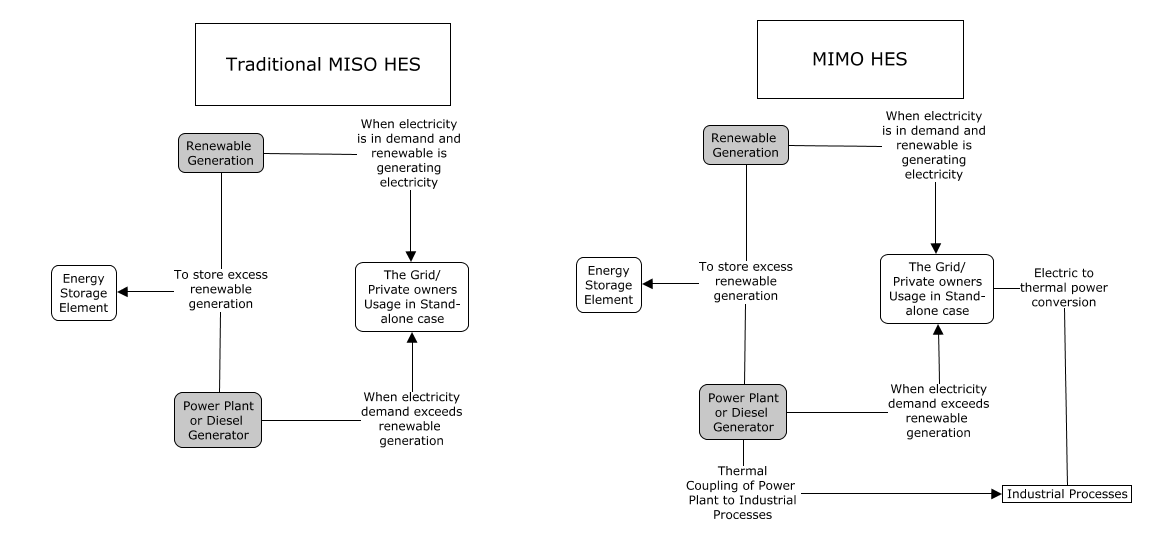
\includegraphics[width=\textwidth]{MISO_MIMO.png}
\caption{\small \sl This figure compares the MISO and MIMO configurations, demonstrating the differences between traditional hybrid energy systems that are focused on generating reliable electricity and non-traditional hybrid energy systems, which have the added objective of generating an additional product.  While many of the elements are the same, the MIMO system includes an Industrial Process  that is either thermally or electrically coupled.}
\end{figure*}

\section{Nuclear Renewable Hybrid Energy Systems}
Nuclear Renewable Hybrid Energy Systems (NRHES) are defined by Bragg-Sitton et al. (2014) as the 

\begin{quotation}
"tighter coupling of nuclear and renewable energy sources in a manner that better optimizes energy use for the combined electricity, industrial manufacturing, and transportation sectors capable of apportioning thermal electrical energy to first meet the grid demand (with appropriate power conversion systems), then utilizing excess thermal and, in some cases, electrical energy to drive a process that results in an additional product \cite {Bragg-Sitton2014}".
\end{quotation}

The benefits to the participants of the NRHES that co-locate their facilities include minimizing system wide costs to the NRHES while increasing economic resilience by diversifying both the means of generating energy as well as the products produced. For example, if natural gas prices increase, the NRHES could rely less on the natural gas plant and put more focus on storage.  If short-term electricity prices are negative, the energy produced by the NRHES can be diverted to the industrial process.  

The additional industrial products possible to couple in a NRHES include, but are not limited to: synthetic fuel, titanium, desalinated water, hydrogen, aluminum, and heat pumps \cite{Bienvenue2015}. The NPP diverts the energy it generates between the grid and the industrial process to maximize profit. The system can allocate energy based on the market value of each of the multiple outputs produced. In the case of a NPP coupled with a desalination plant, for example, if the price of electricity is low, more thermal and/or electric energy can be diverted to generate more clean water at a higher profit \cite {Chen2016}. The costs of running a dynamic system, such as the case with a NRHES, include additional wear and tear, decreased thermal efficiency  due to variability, and increased complexity of operations  \cite{Garcia2013}. The total net costs of the system, such as meeting regulatory expectations, have yet to be determined. 

\section{Ongoing Modeling Research}
There have been no physical demonstrations to date of NRHES. Therefore, research has largely focused on computational modeling to determine the feasibility and optimization of coupling elements \cite{Rabiti2015, Boardman2013, Shropshire2012}. The literature review revealed that much of the work on NRHES is in the design and analysis stage \cite{Epiney2016, Boardman2013, Shropshire2012}. Research has focused on developing models that can dynamically simulate the contributions of variable energy sources, the constraints of fluctuating electricity demand, and thermal/electrical power demands for various industrial processes. The models focus on answering questions regarding minimizing the cost of electricity and ensuring profitability for each of the components comprising the NRHES. In order to move forward with development of any NRHES, such systems must demonstrate that they can be profitable and can reliably respond to fluctuating electricity production and demand \cite{Rabiti2015}. 

An ongoing effort at \ac{inl}, \ac{anl}, and \ac{ornl} focuses on modeling a generic NRHES to optimize the size of the components as well as the overall functioning of the system. The generic nature of the plant means that regional variability in the renewable energy produced as well as the costs of the feedstocks for each of the systems is not taken into consideration. The generic model will test the economic viability of NRHES to determine if future development should be pursued. The industrial plant combines a nuclear power plant, a wind farm, a natural gas power plant, a battery, and a high temperature steam electrolysis hydrogen production facility. More component models will be developed in the future that can compare various industrial customers\cite{Harrison2016}. The chosen renewable source, a wind farm, models a highly stochastic system due to the unpredictable nature of wind generation \cite{Chen2016_wind}. The model optimizes the sizes of the nuclear power plant, the natural gas plant, and the battery. The model performs two optimizations, the first on the size of the components and the second optimizing the functioning of the system to minimize costs \cite{redfoot_rabiti_2018}. The objective is to choose the NRHES configuration that minimizes costs while meeting set emissions and grid reliability expectations.

\section{Computational Tools}
NRHES sit in an interesting location in computational modeling. There are many tools to model and optimize non-nuclear hybrid energy systems (HOMER, Hybrid2, SOLSIM, SOMES, ARES, RAPSIM, HOGA) \cite {Bernal-Agustin2009}. These programs calculate mass flow, electricity output, and the possible output of another product, such as hydrogen. Modelica and Excel, while neither specifically HES nor NRHES tools, have been used to model both nuclear and non-nuclear hybrid energy systems \cite{Shropshire2012, Chen2016, Binder2014, Garcia2015, Epiney2016}. HES tools have typically been developed for microgrid standalone systems. The main challenges to applying HES systems to a NRHES are the scale of the system being modeled and fluctuating grid demand. 

\section{NRHES Models}
Selecting a tool to model a NRHES requires understanding what characteristics a model must possess in order to provide accurate information. For example, as discussed below, it is important for a NRHES model to incorporate the dynamic nature of the system in order to include losses from the fluctuations in the system. Rabiti et al. (2015) discusses the important elements of a NRHES computational model in detail, describing the basic requirements of the software as a 

\begin{quotation}

"computational representation of the thermal, mechanical, chemical, and electrical processes in the systems as process units, reactors, manufacturing plants, and energy delivery (to the appropriate point of interface with the market transaction, such as an electricity bus, or a product depot or distribution terminal where a commodity price is established)"\cite{Rabiti2015}.
\end{quotation}

The model in development by the national laboratories combines \ac{raven} for the stochastic and statistical aspects of the system, such as generating synthetic wind data and optimizing the systems, with Modelica for modeling the various components in the NRHES.

\subsection{Modelica}
Modelica is a widely used open source language for modeling large and complex systems composed of smaller component models. It is particularly optimized for modeling dynamic systems. Modelica has powerful libraries, such as Thermopower, that include the thermohydraulic modeling tools required for modeling mass flows in energy systems \cite{Binder2014}. The language is well-maintained, giving it the added benefits of having up-to-date documentation and a community that can provide support. Typically Modelica is run on the Dymola developer environment, a private tool developed by the creator of Modelica, Dr. Hilding Elmquist. Another option for running the Modelica language is the open source OpenModelica environment.

A Modelica HES model developed in Binder et. al. (2014) includes a nuclear reactor, two steam cycles, a chemical plant, and an electrical component \cite{Binder2014}. The products of this Modelica NRHES model are synthetic fuel and electricity. The model includes the ramp up stage when the reactor initially starts or is increasing from a lower load. The steam generator connected to the NPP determines which of its turbines to use depending on electricity demand, the 60\% turbine, the 30\% turbine, or the 15\% turbine, which can be used in unison. A pressure relief valve releases excess energy unused by the turbines. The wind generation is modeled using the Western Wind dataset from the \ac{nrel} for an unspecified region in Idaho. Each component in the model was tested individually before being combined. Using the individual component models, verifications were made for the system as a whole. The startup transient state of the model took much greater computation time due to the complex interrelations of the components. Generally, running a model of a NRHES in Modelica requires a control algorithm, a differential equation that controls how the dynamic system allocates heat. The profitability control algorithm can be adjusted to incorporate varying parameters such as the price of electricity or the cost of natural gas. The study concluded that Modelica, due to its ability to evaluate control algorithms, is an effective tool for dynamically modeling a HES. As a tool that is optimized for large dynamic systems, Modelica has been used more than any other tool to model NRHESs at this point.  

\subsubsection{RAVEN}
The RAVEN tool was initially built for probabilistic risk assessment. RAVEN, as a probabilistic tool, can do parametric and stochastic analyses of systems\cite{RabitiRAVEN}. For the NRHES, RAVEN is used to run different wind energy generation paths in order to generate a statistically fair representation of how renewables, in this case wind power, would likely function over any given week. RAVEN can be used to produce data representing the most generic seasonal wind generation over a week. A typical week can be extrapolated to represent a given season. The process can be repeated over the different seasons, which can be extrapolated to represent a year. Using synthetic generated data instead of historic data avoids the critique that the model only represents past behavior and is thus inapplicable to future trends \cite{redfoot_epiney_2016}. RAVEN can also be used to determine high-risk time series samples to ensure that high risk scenarios are accounted for in the study. RAVEN can also do probabilistic assessments such as loss of load probability and sensitivity to uncertainty analysis. 

Any future modeling efforts for a NRHES would benefit from complimenting the ongoing modeling effort. Currently, all of the physics models for the NRHES are built in Modelica. To benefit from the work already done, any additional software would need to be able to easily communicate with the Modelica modeling language.  The model would benefit from a tool that would communicate with other chemical and utility standard physics modeling tools. Future work would benefit from coupling with other physics modeling tools, allowing groups to take advantage of the existing infrastructure while using their physics model of choice. 

\subsection{Distinct Capabilities}
There are certain characteristics of a physical NRHES which a computational model would need to reasonably assess the system as a whole. Table I below demonstrates the functions which are most commonly incorporated in a model. The below discussion details the extensive work that has been done determining why a dynamic system is important to a NRHES. 

In Garcia et. al. (2013) and Du et. al. (2014), a dynamic approach to modeling hybrid energy systems (HES) is applied in order to appropriately address the impacts of flexible operation of the system due to variable renewable generation \cite{Garcia2013, Du2014}. In Du et. al. (2014), two optimization problems are addressed: the first minimizes variability in the HES through optimizing components of the HES system, and the second imposes operating and capital costs on the design variables. Garcia et. al. (2013) has a two-part series. The first applies and analyzes performance of a dynamic approach to modeling some of the physical components of a traditional and an advanced MIMO HES. The second paper focuses on economic effects using a dynamic approach, as opposed to time series or statistical analysis. Overall, both parts of the series focus on how a dynamic approach better models the high level of variability of a HES for output generation and profitability maximization \cite{Garcia2013}. The costs of operating in a flexible manner, dynamically allocating resources between multiple coupled systems, are substantial enough to require a simulation that precisely models the variability of the system \cite{Garcia2013, Shropshire2011, Locatelli2015}. The dynamic modeling at this point focuses on the dynamic transfer of energy to different sources, and how this impacts the economics and grid reliability. The physical impacts of the grid system have not yet been included in the most developed NRHES simulation, the national laboratory model \cite{Harrison2016}.  The dynamic allocation of the heat and electricity depending on the renewable generation and the grid demand is an essential characteristic of a NRHES.  Including factors such as how quickly the NRHES will be able to switch between providing energy to the industrial facility and the grid will impact determining the economic and physical values of the model.

\section{Small Modular Reactors}
For completeness, the use of \ac{smrs} both as tools for load following and as sources of process heat must be addressed. SMRs are generally defined as nuclear reactors under 300 MWe. SMR designs, such as that in development by NuScale, combine multiple small reactor modules. Multiple SMRs in combination are a promising possibility for NRHES.  With multiple reactors, individual modules can be assigned to meet the industrial process energy demand, with others solely used for electricity generation. Furthermore, as electricity demand grows, additional modules can be added to the industrial park. Multiple SMRs have a clear means of load following, simply by shutting down those reactors whose energy output is not required due to seasonal shifts and other demand factors. The modularity of the SMRs allows greater flexibility in the design of the industrial park.  Locatelli (2015) discusses the technical and economic feasibility of load following using multiple SMRs, applying the excess energy toward generating algae-biofuel and desalinated water \cite{Locatelli2015}. He discusses the benefits as well as drawbacks of an NRHES that includes a thermal desalination process. A desalination plant has the benefits of switching between a latent and producing state and generating a product that is readily stored. The main drawback is poor water quality and output level when the desalination unit restarts. In general, SMRs have multiple means of adjusting their electricity output to the grid including coupling with an industrial process.

The NuScale reactor, with proposed construction starting in 2025 at INL, has motivated research into different methods of fluctuating the amount of electricity sent to the grid \cite{Ingersoll2014, Ingersoll2015, Ingersoll2016, Ingersoll2014_1}. The NuScale reactor design, as can be seen in the figure below, combines twelve small pressurized water reactors into one large pool of water.  Each of the reactors is rated at 50 MWe,generating a combined 600 MWe. The NuScale reactor has been evaluated to thermally couple with oil refining processes, multiple desalination techniques, as well as hydrogen production \cite{Ingersoll2014}. Besides from thermally coupling and rerouting the energy from electricity generation to process heat applications, the NuScale reactors have furthermore been evaluated for loosely coupling with the Horse Butte Wind Farm in nearby Idaho Falls \cite{Ingersoll2015}.  The NuScale plant has multiple approaches to meet the fluctuating electricity demanded by the grid, which NuScale designates as NuFollow \cite{Ingersoll2015}.  The NuScale plant can take down one or more of the low power reactors, changing the power output of one or more modules for shorter changes in the grid demand due to changes in wind output, and sending the heat generated by the reactor straight to the condenser bypassing the power generating turbine cycle.  
\begin{figure*}[h!]
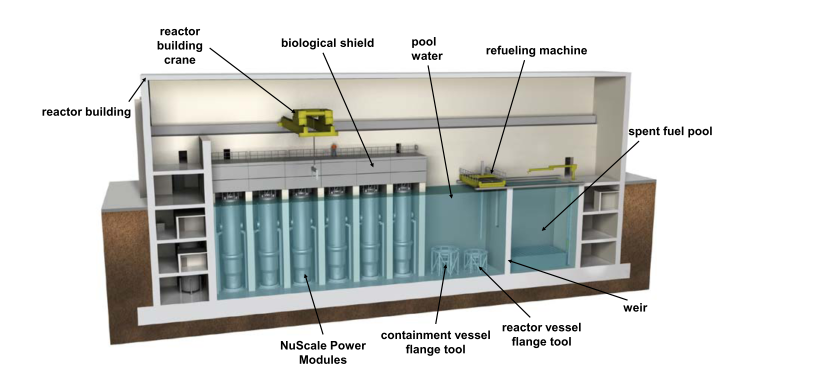
\includegraphics[width=\textwidth]{NuScale_cutaway.PNG}
\caption{\small \sl This figure displays the design of half of the NuScale module. Six of the reactor modules can be seen in the cooling pool along with the crane which inserts and removes the modules.}
\end{figure*}
\subsection{Other Research on NRHES Models}
Many more studies on HES and NRHES incorporate economic and technical modeling, but the essential characteristics of ability to model a dynamic and stochastic system have been covered. For completeness of the state of the art research on NRHES, some of the other relevant studies include: 
\begin{itemize}
\item Shropshire et. al. (2012) does not focus on HES, but discusses how different models of flexible and small modular reactors could integrate into the European energy market with growing renewable generation, thus fulfilling the growing need for flexibility and load following in other electricity suppliers \cite{Shropshire2012}. 
\item Shropshire et. al. (2011) develops target cost estimates for reactors given certain economic environments based on competing technology energy costs \cite{Shropshire2011}. 
\item NEA-OECD (2011), Nuclear Energy Agency Organisation for Economic Co-operation and Development, presents an overview of the capability of implemented newer and older nuclear power plants to load follow \cite{Nuclear2011}. 
\item Baker (2016) analyzes the \ac{lcoe} as the \ac{fom} and the role of battery storage to evaluate different NRHES scenarios \cite{Baker2016}
\item Kazimi et al. (2009) produces a preliminary dynamic analysis of two NRHES systems that have high levels of renewable energy generation and multiple outputs from the system. The study concludes that NRHES could lead to optimized energy use, reduced carbon, favorable economic performance, and flexible operation time \cite{Kazimi}. 
\item Forsberg et. al. (2009) discusses using nuclear power to create more liquid transportation fuels from biomass and fossil fuel sources \cite{Forsberg2009}. 
\item There have also been two regional modeling studies done on Texas and Arizona focused on including regional characteristics to determine the renewable used and the industrial process.  
\end{itemize}
Table I displays the characteristics routinely described as necessary to model a NRHES along with their citations.

\begin{table}[h!]
\centering
\caption{References for Each NRHES Characteristic}
\begin{tabular}{ ||c | c|| }
 \hline 
 NRHES Characteristic & Paper \\ [0.5ex]
 \hline \hline
 Dynamic & \cite{Garcia2013, Du2014, Kazimi, Garcia2016}\\
 \hline
 Sensitivity Analysis & \cite{Shropshire2011, Rehman2010, Adaramola2014, Chen2016}\\
 \hline
 Optimization of components & \cite{Chen2016,Ozcan2016, Forsberg2009,Garcia2015,Aumeier2011}\\
 \hline
 Stochastic Model of Renewables & \cite{Rabiti2015, Garcia2016,Locatelli2015}\\ 
 \hline
 Grid Demand model & \cite{Forsberg2013, Garcia2016,Garcia2013,Ruth2014,Chen2016}\\
 \hline
  Economic FOMs & \cite{Garcia2016,Chen2016,Rabiti2015,Epiney2016,Bragg-Sitton2014}\\
 \hline
\end{tabular}
\label{table:1}
\end{table}

The table displays the characteristics that arise as a pattern in many of the documents.  The six characteristics included in the table are those likely necessary for a NRHES model.  Each of the characteristics has been included in previous studies, and thus has some already proposed approaches.  The characteristics can be studied in greater detail in order to determine if they satisfactorily model the system.


\chapter{Applying Risk Assessment Techniques to NRHES}
\label{AHPChapter}
Identifying likely failures is an important aspect of safe and secure operation of any large infrastructure. For a NRHES, a large piece of infrastructure that has as of yet to be built, a design that addresses likely failures ensures long term safe, reliable, and profitable operation. This chapter will evaluate the economic, grid reliability, and physical risks of failures in the coupling of a nuclear power plant to an industrial process which functions in a dynamic fashion. Three preliminary hazard analyses will initially be applied to the safety, ability to fluctuate, and profitability of the system in order to do a cursory qualitative model of what concerns need to be taken into consideration. A fuzzy Analytic Hierarchy Process (f-AHP) will then be applied to various industrial process options to couple with an NRHES. The focus of this section is to develop a means of comparing various NRHES industrial processes to determine which industrial process will be used in the exergy analysis. 
\section{Risk Assessment Background}
Risk assessment is a means of analyzing complex systems for hazards. Often the risk assessment tools; such as probabilistic risk assessment, fault tree analysis, and failure mode and effects analysis; model many variables in large systems and attempt to contain them into an easy to understand table or number for comparison. Since there has yet to be a physical model of a NRHES built, now is the appropriate time to assess risks in order to incorporate mitigating measures in the design basis. Incorporating risk management in the design of a facility minimizes the costs and dangers associated with the system in the long run.
%When determining an appropriate electricity generation source for a given region it is important to incorporate variables such as economic viability, emissions, flexibility, and reliability. A NRHES is even more difficult to quantify as it supplies both electricity to the grid as well as a secondary product. The goal is to have a more economically robust system that emits less and is both more reliable and more flexible than any electricity generation source currently available. 

\section{Preliminary Hazards Analysis}
As was done in Falcone et. al. in establishing a new approach to risk assessment of cogeneration systems, this risk assessment will begin with a \ac{pha} \cite{Falcone}. The main purpose for a PHA is, as the name suggests, identify hazards and possible implications of the design of a particular system or product.  A PHA is appropriate for the current state of development for a NRHES due to it still being in the design stage. The goal of this PHA will be to highlight potential economic, reliability, and physical safety hazards. Performing a PHA at this early point in the life cycle of a NRHES will hopefully reduce the resources spent on engineering design and potential construction errors. This analysis is not exhaustive but will address some of the more obvious concerns. The PHA will need to be added upon as research continues and hazards are determined. 
	In order to perform a PHA requires classifying the hazard level and frequency associated with each event. The hazard classes for this PHA range from Negligible to Catastrophic. A Class I hazard has negligible negative outcomes, a Class II hazard has marginal effects, a Class III hazard has critical impacts, and a Class IV hazard has catastrophic impacts\cite{ostrom2012risk}.  The frequency of occurrence, since this system has yet to have a physical demonstration, will be qualitative as the values cannot be verified at this point. A discussion of the tables follows after tables \ref{econ, fluc, safety} below. 

\begin{landscape}
%\subsubsection{Economic PHA}
\begin{table}[h!]
\centering
\caption{Economic Preliminary Hazard Analysis}
\label{econ}
\begin{tabular}{|l|l|l|l|l|l|}
\hline
\textbf{\begin{tabular}[c]{@{}l@{}}Potential \\ Failure\end{tabular}} & \textbf{\begin{tabular}[c]{@{}l@{}}Event Causing\\ Hazardous\\ Condition\end{tabular}} & \textbf{\begin{tabular}[c]{@{}l@{}}Hazardous\\ Condition\end{tabular}}  & \textbf{Hazard Class} & \textbf{\begin{tabular}[c]{@{}l@{}}Preventative \\ Measure\end{tabular}} & \textbf{\begin{tabular}[c]{@{}l@{}}Qualitative\\ Likelihood\end{tabular}} \\
\hline 
\begin{tabular}[c]{@{}l@{}}Industrial process\\ is not profitable \end{tabular}      & \begin{tabular}[c]{@{}l@{}}If the industrial\\ process has to be\\ ready to take load\\ from the grid, it \\ will likely be running\\ below capacity and \\ may not be profitable\end{tabular}      & \begin{tabular}[c]{@{}l@{}}Industrial \\ process loosing\\ money\end{tabular} & \begin{tabular}[c]{@{}l@{}}Class III,\\ the benefit of\\ the NRHES \\ would be lost\\ without a means\\ of having the \\ industrial process\\ prepared to take \\ heat. \end{tabular}    & \begin{tabular}[c]{@{}l@{}}Contracts \\ ensuring\\ a certain profit\\ for the industrial\\ process to be \\ prepared to \\ take heat from\\ the Nuclear\\ Power Plant\end{tabular} & Likely \\
\hline
\begin{tabular}[c]{@{}l@{}}Nuclear regulations \\ could apply to the\\ whole system, \\ increasing the costs\\ of the system\end{tabular} & \begin{tabular}[c]{@{}l@{}}Since the \\ components will \\ be co-located \& \\ coupled, the NRC \\ may have\\ jurisdiction \\ over the whole system\end{tabular}  & \begin{tabular}[c]{@{}l@{}}Additional \\ regulations \\ on the industrial \\ process could \\ result in greater\\ costs\end{tabular} & \begin{tabular}[c]{@{}l@{}}Class III: without an \\ industrial process\\ the whole NRHES \\ would be undermined.\end{tabular} & \begin{tabular}[c]{@{}l@{}}Determine regulatory \\ oversight before \\ beginning \\ construction\end{tabular} & \begin{tabular}[c]{@{}l@{}}Fairly Likely\\ as the other\\ components\\ would be\\ within the\\ required \\ boundary \\ around the NPP\end{tabular} \\
\hline
Feedstock costs rising & \begin{tabular}[c]{@{}l@{}}Any of the feedstocks\\  could rise in price for \\ any number of reasons. \\ Rise in price during \\ the operation of the \\ system could result in \\ the product prices no \\ longer being\\ competitive\end{tabular} & \begin{tabular}[c]{@{}l@{}}Feedstocks rising in \\ price during the \\ operation of the system \\ could\\ result in the \\ product prices no \\ longer being \\ competitive\end{tabular} & \begin{tabular}[c]{@{}l@{}}Class I: shifts \\ already occur in\\ feed stock prices and\\ are systems adjust.\end{tabular}  & \begin{tabular}[c]{@{}l@{}}Include long term \\ projections for the \\ feedstock costs of \\ the various \\ components in the \\ design phase of the \\ NRHES\end{tabular}                      & \begin{tabular}[c]{@{}l@{}}Likely there \\ will be \\ fluctuations.\\ Depends on the \\ feedstock\end{tabular}\\
\hline
Product value decreasing & \begin{tabular}[c]{@{}l@{}}There could be a \\ change in \\ conditions or a \\ new technology \\ that makes the \\ industrial process \\ product value \\ decrease\end{tabular} & \begin{tabular}[c]{@{}l@{}}For each of the products,\\ the reason would be \\ different. Desal: a \\ drought could end\\ Syn fuel: oil prices \\ could decrease\\ Hydrogen: Less \\ energy\\ intensive \\ process could be \\ invented\end{tabular} & \begin{tabular}[c]{@{}l@{}}Class II: the industrial \\ process would need\\ to be further subsidized\\ by other components \\ to continue to run\end{tabular}& \begin{tabular}[c]{@{}l@{}}Do long term \\ economic \\ analysis of the \\ industrial \\ process. Pick \\ a product \\ or location where\\ the product will \\ clearly be in demand\end{tabular} & \begin{tabular}[c]{@{}l@{}}Possible: The \\ product value \\ will likely \\ fluctuate over \\ the length of \\ the\\ project\end{tabular}          \\ \hline
\end{tabular}
\end{table}                                           \end{landscape}                                                       



\begin{landscape}
%\subsection{Grid Reliability PHA}
\begin{table}[h!]
\centering
\caption{Grid Reliability Preliminary Hazard Analysis}
\label{fluc}
\begin{tabular}{|l|l|l|l|l|l|}
\hline
\textbf{\begin{tabular}[c]{@{}l@{}}Potential \\ Failure\end{tabular}} & \textbf{\begin{tabular}[c]{@{}l@{}}Event Causing\\ Hazardous\\ Condition\end{tabular}} & \textbf{\begin{tabular}[c]{@{}l@{}}Hazardous\\ Condition\end{tabular}} & \textbf{Hazard Class} & \textbf{\begin{tabular}[c]{@{}l@{}}Preventative \\ Measure\end{tabular}}  & \textbf{\begin{tabular}[c]{@{}l@{}}Qualitative\\ Likelihood\end{tabular}} \\
\hline
\begin{tabular}[c]{@{}l@{}}Nuclear Power \\ Plant Outage\end{tabular}  & \begin{tabular}[c]{@{}l@{}}The NPP needs \\ to be refueled\end{tabular} & \begin{tabular}[c]{@{}l@{}}NPP down for \\ refueling\end{tabular} & \begin{tabular}[c]{@{}l@{}}Class I: This will \\ be a routine issue. \\ The industrial \\ process will need \\ to stop during the \\ outage and the \\ grid will need to \\ get electricity \\ from peaker\\ plants\end{tabular} & \begin{tabular}[c]{@{}l@{}}Plan ahead with the \\ industrial process \\ so that it can either \\ get\\ electricity from\\ the grid or be \\ paid to close for \\ the outage.\end{tabular}                                     & \begin{tabular}[c]{@{}l@{}}Certain: an \\ NPP needs to \\ be refueled\end{tabular} \\
\hline
\begin{tabular}[c]{@{}l@{}}System not able \\ to quickly shift\\  heat from \\ industrial process \\ to\\ electricity \\ generation\end{tabular} & \begin{tabular}[c]{@{}l@{}}The NPP heat \\ transport system \\ taking a while to \\ shift.\end{tabular} & \begin{tabular}[c]{@{}l@{}}The NRHES is \\ briefly unable \\ to meet \\ the grid demand\end{tabular} & \begin{tabular}[c]{@{}l@{}}Class II: There \\ would be some \\ money loss as \\ some other \\ electricity \\ generation system \\ would supply the \\ demanded energy \\ during the transition \\ period\end{tabular}            & \begin{tabular}[c]{@{}l@{}}Include the time it \\ takes to allocate \\ heat in models of \\ the NRHES to \\ determine how \\ much of a limiting \\ factor it is likely to be.\\ Include a battery in\\ the NRHES\end{tabular} & Likely \\                       \hline   
\end{tabular}
\end{table}
\end{landscape}



\begin{landscape}
%\subsection{Physical PHA}
\begin{table}[h!]
\centering
\caption{Physical Preliminary Hazards Analysis}
\label{safety}
\begin{tabular}{|l|l|l|l|l|l|}
\hline
\textbf{\begin{tabular}[c]{@{}l@{}}Potential \\ Failure\end{tabular}}                        & \textbf{\begin{tabular}[c]{@{}l@{}}Event Causing\\ Hazardous\\ Condition\end{tabular}} & \textbf{\begin{tabular}[c]{@{}l@{}}Hazardous\\ Condition\end{tabular}} & \textbf{Hazard Class} & \textbf{\begin{tabular}[c]{@{}l@{}}Preventative \\ Measure\end{tabular}} & \textbf{\begin{tabular}[c]{@{}l@{}}Qualitative\\ Likelihood\end{tabular}}                 \\
\hline
\begin{tabular}[c]{@{}l@{}}Materials failure \\ in the heat \\ transport system\end{tabular} & \begin{tabular}[c]{@{}l@{}}NRHES are very \\ dynamic systems. \\ There will likely \\ be greater materials \\ wear due to the \\ dynamisticity of \\ the system\end{tabular} & \begin{tabular}[c]{@{}l@{}}Heat transport \\ pipe forms a leak\end{tabular}            & \begin{tabular}[c]{@{}l@{}}Class III:There \\ would be a loss \\ of\\ money due \\ to the shutdown \\ of the system\end{tabular}                                                                                                          & \begin{tabular}[c]{@{}l@{}}Reliable maintenance \\ \& appropriate choice \\ of heat transport \\ system\\ materials\end{tabular} & Possible                                                                                  \\
\hline
Release of Radionuclides                                                                     & \begin{tabular}[c]{@{}l@{}}Radionuclides \\ would need to \\ escape first into \\ the heat transport \\ system and then from \\ the heat transport system \\to the environment\end{tabular}                                                                                          & \begin{tabular}[c]{@{}l@{}}A large release \\ of airborne\\ radionuclides\end{tabular} & \begin{tabular}[c]{@{}l@{}}Class IV: A \\ radiation release \\ that could \\ potentially impact \\ human health \\ would have\\ massive negative \\ impacts for the \\ nuclear industry \& \\ would shut down \\ the\\ NRHES\end{tabular} & \begin{tabular}[c]{@{}l@{}}Passive safety \\ systems, excellent \\ safety culture, \\ good reactor design\end{tabular}           & \begin{tabular}[c]{@{}l@{}}Unlikely: Based \\ on history of \\ NPP operation\end{tabular} \\
\hline
\end{tabular}
\end{table}
\end{landscape}

The initial economic PHA, table \ref{econ}, demonstrates the importance of having detailed agreements between the various members of a NRHES industrial park before construction begins.  Likely, the whole system would function better under a single owner.  A single owner could allow an aspect of the NRHES, such as the industrial process, to loose money and still be economic overall. Further avenues which need to be investigated before the construction of an industrial park include understanding the regulatory impacts and the long term projected worth of the products generated.

The initial grid reliability PHA, table \ref{fluc}, demonstrates the importance of understanding how coupling an NPP to an industrial process will require a change of the scheduling approach to a nuclear power plant. Nuclear power plants require immense amounts of planning and scheduling in order to ensure safe operation of the plant.  Increasing the complexity through coupling the nuclear power plant to other systems will increase the complexity of scheduling activities such as outages as well as optimizing the heat and electricity output of the system to match the grid demand. 

The initial physical PHA, table \ref{safety},  demonstrates how, if done correctly, a thermally coupled industrial process to a nuclear power plant does not have to increase the danger of the system.  Since nuclear power plants already have a lot of techniques in place to ensure a safe system that will not harm the public or the environment, those same approaches should be applied to the thermally coupled system. The existing infrastructure, including the safety culture, could be extended to the thermal coupling. Thermal coupling is used throughout this thesis as the use of heat from the \ac{npp} used directly for an industrial process.  Electrical coupling, for comparison, takes the electricity generated by the \ac{npp} which is then used to do electrical work or converted into heat or mechanical work to produce the desired product in the industrial process. 


\section{Analytic Hierarchy Process}
The fuzzy AHP done in this research compares NRHESs that include thermal coupling to three types of industrial processes: desalination, synthetic fuel production, and hydrogen production.  The AHP evaluates the profitability, flexibility, and safety characteristics in the coupling of a nuclear power plant to each of the given industrial processes. While AHP has been applied to energy systems in the literature, the application to NRHES is novel. An AHP approach provides important information into design considerations and quantitatively approaches, through expert opinion, which alternative is likely to be strongest given the criteria chosen. As NRHESs are currently in the research and development stage, AHP is a beneficial tool to develop for future decision making for NRHES. 

An AHP uses pairwise comparisons of various potential options depending on a set of predetermined characteristics. Originally developed in the 1970s by Thomas L. Saaty, AHP has been applied to everything from determining appropriate bridge construction \cite{Pan2008}, to the appropriate energy make-up of Turkey\cite{Kahraman2010} \cite{Saaty1987}. AHP is a multicriteria decision-making tool. There is a wealth of research applying multicriteria decision-making tools to energy planning. Pohekar et al. reviewed more than 90 published papers on multi-criteria decision making and energy planning \cite{Pohekar2004}. Pohekar et al. found AHP to be the most popular multicriteria decision-making technique used in energy planning. The reasons for the prevalence of AHP in energy planning, Pohekar et al. suggests, is due to its ability to: 
\begin{quote}
	"convert a complex problem into a simple hierarchy, flexibility, intuitive appeal, its ability to mix qualitative as well as quantitative criteria in the same decision framework and use of computational aids leading to successful decisions in many domains.\cite{Pohekar2004}"
 \end{quote}
Some of the previous applications of AHP to energy systems noted in Pohekar et al. include Akash et al.  1999; and Ramanathan et al. 1995. Akash et al. uses AHP to analyze the selection of power plants in Jordan \cite{Akash1999}.  Ramanathan et al. applies AHP at a household level in India to determine which energy resources work best for various tasks in the home such as heating, water pumping, lighting, and household appliances \cite{Ramanathan1995}.  

The general process for applying AHP involves initially determining a set of alternatives and a set of criteria on which to compare the alternatives. The hierarchy comes from the objective being structured above the criteria, which is then structured above the alternatives, as can be seen in figure 3.1 below. To find the relative value of one of the alternatives over the other, the AHP approach develops a series of pairwise comparisons creating a ratio scale.  Generally AHP is done on a scale of one to nine. After creating the ratio scale, the AHP approach applies an eigenvalue method to include the relative weights of each of the criteria to each of  the elements. Finally, the relative weights are combined with the ratios forming one measurement to compare the various elements.

\begin{figure}[h!]
  \centering
  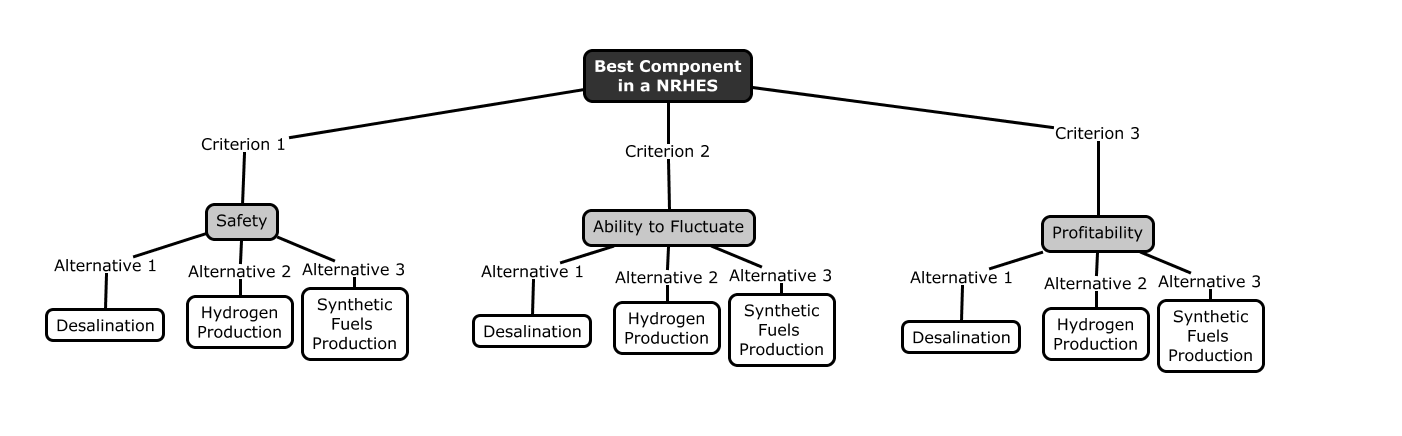
\includegraphics[width=0.9\textwidth]{AHP_hierarchy.PNG}
  \caption{A figure displaying the overall hierarchy of the industrial processes under evaluation for inclusion in the NRHES}
\end{figure}

The AHP provides not only insight into which is the best overall choice given the inputs and weights, but also which is the strongest candidate for each of the criterion. During the AHP process, before aggregating the values into one measurement, there are clear measurements of each of the alternatives in each of the criterion. The subjective nature of expert judgment as data requires a means of evaluation. As a check on the validity of the data,a traditional AHP measures the consistency of the values given by the experts using a Consistency Ratio, which needs to be less than .1, or 10\%, in order to be considered consistent. The Consistency Ratio compares the randomness of the expert judgments to a Random Consistency Index \cite{Saaty1987}.  If the consistency ratio is greater than .1, the data is judged to be too close to random.


\section{Fuzzy AHP}
Fuzzy logic applied to AHP takes into consideration the uncertainty inherent in a small number of expert opinions. Fuzzy AHP is an extension of the original AHP developed by Saaty in the 1970s \cite{Saaty1987}. Since Saaty's original development of AHP, multiple means of fuzzy AHP have emerged. Some notable fuzzy AHP approaches, as noted in \cite{Kahraman2010} include:
\begin{itemize}
\item Van Laarhoven and Pedrycz's approach from 1983 using triangular membership functions
\item Buckley's 1985 use of trapezoidal membership functions to determine fuzzy priorities
\item Cheng's 1997 approach focused on the grade value of the membership function. 
\item Kahraman et al. generated a fuzzy weighted evaluation \cite{Kahraman2010}
\item Chang presented a new approach first determining triangular fuzzy numbers, then applying extent analysis method \cite{Chang1996} 
\end{itemize}
 
 In the Buckley approach to fuzzy AHP, which is applied in this paper, $\alpha$ represents a value between zero and one reflecting the uncertainty.  Uncertainty is greatest when $\alpha$ is close to zero and least when close to one. As can be seen in the figure below, in a trapezoidal membership approach, the lower left point of the triangle, where $\alpha$ equals zero, is the minimum fuzzy number, the points making up the middle represent the most likely fuzzy number, and the point at a y value of zero on the right represents the maximum fuzzy number \cite{Pan2008}. The higher the fuzzy number on the x axis, the more important that criteria is, or the stronger the alternative. 
\begin{figure}[h!]
  \caption{A figure displaying the meaning behind the membership function graph for the fuzzy numbers}
  \centering
  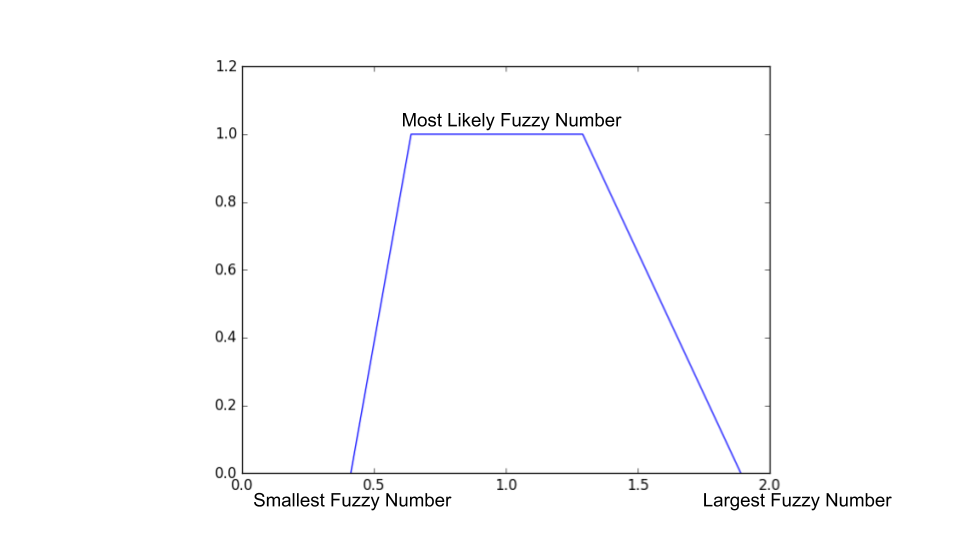
\includegraphics[width=0.9\textwidth]{Fuzzy_explaination.png}
\end{figure}
 
 As described in \cite{Kahraman2010}, after receiving the numbers from the decision makers, the fuzzy weight can be found by determining the geometric mean for each row in each of the AHP matrices:
 
 \begin{equation}
 z_i=[\prod_{j=1}^n t_{ij}]^{\frac{1}{n}}
 \end{equation}
 
 Where $t_{ij}=(a_{ij},b_{ij}, c_{ij}, d_{ij})$ correspond to the fuzzy values in Table 1 below. $n$ is the number of values in each row.  For example, if three experts were taking a survey with three pairwise comparisons, there would be nine total answers in each row. To find the performance scores ($r$), first sum each of the geometric means in each row, then weight each of the values accordingly:
 
\begin{equation}
r_{ij}=(\frac{a_i}{d},\frac{b_i}{c},\frac{c_i}{b},\frac{d_i}{a})
\end{equation} 

To find the fuzzy utility:

\begin{equation}
U_i=\sum_{j=1}^n w_j*r_{ij}
\end{equation} 

where w is the weight found by the comparison of the importance of the various criteria to one another. To find the membership function $M(x)$, take the lowest value of the utility set and set the membership function to zero.  For the middle values of the utility set, the membership function is one. For all values greater than the greatest member of the utility set, the membership function is zero. For a utility set $(x_1,x_2,x_3,x_4)$

\begin{center}
\begin{tabular}{ |c|c| } 
 \hline
 x & M(x)\\
 \hline
 $\leq x_1$  & 0 \\ 
 $\geq x_4$ & 0  \\ 
 $x_2 \leq x \leq x_3$ & 1  \\ 
 $x_1 \leq x \leq x_2$ & $\alpha \in [0,1]$\\
 $x_3 \leq x \leq x_4$ & $\alpha \in [0,1]$\\
 \hline
\end{tabular}
\end{center}

\begin{table}[h!]
\centering
\caption{Fuzzy Logic Value Mapping}
\label{Fuzzy values}
\begin{tabular}{|l|l|l|}
\hline
\textbf{Description }                                                           & \textbf{Values }       & \textbf{Inverse}           \\
\hline
Equal                                                                  & (1, 1, 1, 1)     & (1, 1, 1, 1)         \\
\hline
Equal Importance                                                       & (1/2, 3/4, 5/4, 3/2) & (2/3, 4/5, 4/3, 2)      \\
\hline
Weak Importance                                                        & (1, 3/2, 5/2, 3)   & (1/3, 2/5, 2/3, 1)   \\
\hline
Strong Importance                                                      & (2, 5/2, 7/2, 4)     & (1/4, 2/7, 2/5, 1/2) \\
\hline
\begin{tabular}[c]{@{}l@{}}Very Strong\\ Importance\end{tabular}       & (5, 11/2, 13/2, 7)     & (1/7, 2/11, 2/13, 1/5) \\\hline
\begin{tabular}[c]{@{}l@{}}Absolutely Strong\\ Importance\end{tabular} & (7, 15/2, 17/2, 9)     & (1/9, 2/17, 2/15, 1/7)\\
\hline
\end{tabular}
\end{table}

\section{Expert AHP Survey}
The objective for the expert AHP survey is to determine the optimal industrial process to include in a generic NRHES industrial park based on three criteria. The industrial process options are desalination, high temperature steam electrolysis, and synthetic fuel production. The criteria the options are judged on are ability to fluctuate, safety, and profitability. The optimal way to perform an Analytic Hierarchy Process (AHP) is to gather a group of experts with complementary specializations in a general field to discuss the relative values of various options under determined criteria. For example, performing an AHP to determine the optimal industrial process in a NRHES would best be done by gathering a group of experts in NRHESs with specialties in understanding each of the specific industrial processes. The group could discuss the relative values to give to each of the alternatives for a given criterion. Due to the struggles of getting a group of NRHES experts together in the same place, the values found for this research came from sending a survey to experts.  Other AHP evaluations employ similar methods\cite{Pan2008}. For this research, an expert is defined as someone who has published research or reports on NRHES.

	I chose the alternatives of desalination, hydrogen production, and synthetic fuels production due to their prominent role in research surrounding NRHES \cite{Bragg-Sitton2014,Locatelli2015,Kim2016,Bragg-Sitton2016,Garcia2016,Shropshire2011, Ruth2014,Bienvenu2015}.  I chose the criterion of ability to fluctuate as the industrial process in a NRHES will need to be able to fluctuate to adjust to change demand as well as the dynamic generation from the industrial process.  I chose the criterion of safety due to the inherent need for safety, especially within the context of the nuclear safety culture.  Safety underlies both the characteristic of ability to fluctuate and profitability. If the industrial process is not safe, it will not run, and therefore the other two characteristics are negligible. I chose profitability as clearly the whole NRHES will need to be profitable in order to continue to run.  The industrial process provides a secondary source of income  increasing the overall profitability of the system as a whole. 

There were five experts who completed the Analytic Hierarchy Process for a Nuclear Renewable Hybrid Energy System survey. Due to the small number of experts included in the survey, a fuzzy systems approach has been applied to the AHP. Tsyganok et al. determined that the expert competence should always be taken into consideration, especially when there are less than 50 experts included in the evaluation \cite{Tsyganok2012}. Thus in this case a fuzzy approach is clearly applicable due to the low number of responses.

 For this research, the same NRHES with only the industrial process switched out will be compared. The assumptions for this research include:
\begin{itemize}
\item The process used for hydrogen production is high temperature steam electrolysis with thermal as well as electrical coupling to the nuclear power plant  
\item  The process for desalination is thermal desalination through distillation directly using heat from the nuclear power plant   
\item The synthetic fuel process is a Fischer-Tropsch method using coal as the hydrocarbon source
\item Each of the processes consumes the same amount of heat from the nuclear power plant
\item All of the industrial processes are thermally coupled
\item Regional accessibility of feedstocks for each of the industrial processes are the same
\item Regional transportation costs are the same
\item Regulatory and taxation costs are the same
\end{itemize}
 
As can be seen in Table 2 below, the scale for the answers for the second part of the question ranged from two to  nine.  In the initial question the expert determines which of the alternatives better fits the criteria.  If the two alternatives were judged to equally answer the question, then a value of 1 was assigned to the relative importance of both. Table 3.5 displays the relative values for each of the characteristics considered in the AHP. The values are chosen on a scale of one to nine, with the industrial process strongly reflecting that characteristic receiving a nine and the characteristic relatively less reflecting those characteristics receiving appropriate smaller numbers. While the safety of the system is in reality the most important characteristic, as it is the foundation which the economic and grid reliability characteristics rely on, the safety issues are the most easy to mitigate and the most well known. 

\begin{table}[h!]
\centering
\caption{Example of questions given in the Expert AHP survey}
\label{my-label}
\begin{tabular}{l}
Questions included in the expert AHP survey:                                                                                   \\ \hline
\multicolumn{1}{|l|}{\begin{tabular}[c]{@{}l@{}}Q1a: Do you think that the ability to fluctuate,is more important\\ than profitability of an industrial process?\\ Q1b: From 2 to 9, how would you compare the importance of \\ safety of an industrial process to the ability of the industrial process to fluctuate?\\ Q2a: Do you think that the ability to fluctuate,is more important than \\ profitability of an industrial process?\\ Q2b: From 2 to 9, how would would you compare the importance \\ of safety of an industrial process to the ability of the industrial process to fluctuate?\end{tabular}} \\ \hline
\end{tabular}
\end{table}                                               

\begin{table}[h!]
\centering
\caption{AHP Scale Description}
\label{my-label}
\begin{tabular}{|l|l|l|}
\hline
Quantitative Value & Explanation                                                                                                                              & Verbal Judgement                                                        \\ \hline
1                  & \begin{tabular}[c]{@{}l@{}}They are equally important \\ or equally meet the criterion\end{tabular}                                      & Equally more important                                                  \\ \hline
2                  & \begin{tabular}[c]{@{}l@{}}Experience and judgement \\ favor one alternative over \\ the other by a small margin\end{tabular}            & Weakly more important                                                   \\ \hline
3                  & \begin{tabular}[c]{@{}l@{}}Experience and judgement \\ moderately favor one \\ alternative over the other\end{tabular}                   & Weakly more important                                                   \\ \hline
4                  & \begin{tabular}[c]{@{}l@{}}Experience and judgement \\ clearly favor one \\ alternative over the other\end{tabular}                      & Strongly more important                                                 \\ \hline
5                  & \begin{tabular}[c]{@{}l@{}}Experience and judgement \\ strongly favor one \\ alternative over the other\end{tabular}                     & Strongly more important                                                 \\ \hline
6                  & \begin{tabular}[c]{@{}l@{}}Practice suggests moderate\\ preference for one alternative \\ over the other\end{tabular}                    & \begin{tabular}[c]{@{}l@{}}Very strongly more\\ important\end{tabular}  \\ \hline
7                  & \begin{tabular}[c]{@{}l@{}}One alternative is favored \\ very strongly over the other \\ and has been shown in practice\end{tabular}     & \begin{tabular}[c]{@{}l@{}}Very strongly more \\ important\end{tabular} \\ \hline
8                  & \begin{tabular}[c]{@{}l@{}}It is fairly clear that, in practice\\ one alternative is better than the \\ other\end{tabular}               & \begin{tabular}[c]{@{}l@{}}Absolutely more \\ important\end{tabular}    \\ \hline
9                  & \begin{tabular}[c]{@{}l@{}}The evidence favoring one \\ alternative over the other is of\\ the highest possible affirmation\end{tabular} & \begin{tabular}[c]{@{}l@{}}Absolutely more \\ important\end{tabular}    \\ \hline
\end{tabular}
\end{table} 

\section{AHP Results and Discussion}
As can be seen in table 4, the utility set values which comprise the membership function are highest for desalination. The utility set generates the weighted value for each of the alternatives using the geometric mean method discussed above. As the higher the utility the greater the value, desalination ranks highest of the options for an industrial process given the criteria. As can be seen in Table 5, safety clearly was prioritized.  Due to the high value placed on safety, and the sense that desalination is safer than the alternatives, it follows that it has a greater fuzzy number. Clearly, the heavy weight placed on safety played a major role in determining the outcome. 

While AHP provides a means to compare various options and criteria, it is limited by not including vital information surrounding when a certain standard has been met. In the case of this research, safety and flexibility standards could have been fully met by all of the industrial processes. Safety, instead of being a relative point of comparison, may be better treated as a set of standards to be achieved, such as those presented in the International Organization for Standardization standards for cogeneration \cite{ISO2017}. While desalination is perceived to be a safer industrial process, that does not mean that a synthetic fuel upgrading system or a high temperature steam electrolysis plant is unsafe to couple to a nuclear power plant. The fact that desalination is perceived as safer and more able to fluctuate becomes negligible at that point. AHP is a beneficial tool when determining the relative value between alternatives.  For example, profitability is a valuable characteristic to compare on relative terms.

NRHESs are difficult systems to have a fully developed sense of expertise surrounding. Due to the industrial parks including different components as well as the importance of including technical, economic, and political variables in the decision making. While an AHP is a valuable tool because it is able to include a variety of characteristics from different disciplines, there need to be experts representing each of the disciplines. Furthermore, the more experts included in the survey, the stronger the data and the more likely a valid conclusion can be drawn from the data.
\begin{table}[h!]
\centering
\caption{Utility Set values for each of the industrial processes}
\label{my-label}
\begin{tabular}{|l|l|}
\hline
\begin{tabular}[c]{@{}l@{}}Industrial \\ Process\end{tabular} & Utility Set               \\ \hline
Desalination                                                  & (0.412, 0.641, 1.291, 1.891) \\ \hline
\begin{tabular}[c]{@{}l@{}}Hydrogen\\ Production\end{tabular} & (0.029, 0.047, 0.084, 0.136) \\ \hline
\begin{tabular}[c]{@{}l@{}}Synthetic \\ Fuels\end{tabular}    & (0.086, 0.128, 0.265, 0.437) \\ \hline
\end{tabular}
\end{table}


 

\begin{table}[h!]
\centering
\caption{Performance Scores of Safety for the various industrial processes included}
\label{my-label}
\begin{tabular}{|l|l|}
\hline
Industrial Process                                                    & Safety Performance Score     \\ \hline
Deslination                                                           & (0.309,0.424, 0.708, 0.917)  \\ \hline
\begin{tabular}[c]{@{}l@{}}Hydrogen \\ Production\end{tabular}        & (0.118, 0.162 ,0.277 ,0.390) \\ \hline
\begin{tabular}[c]{@{}l@{}}Synthetic Fuels \\ Production\end{tabular} & (0.139, 0.181, 0.317, 0.459) \\ \hline
\end{tabular}
\end{table}

\begin{table}[h!]
\centering
\caption{Ability to Fluctuate Performance Scores for the various industrial processes included}
\label{my-label}
\begin{tabular}{|l|l|}
\hline
\begin{tabular}[c]{@{}l@{}}Industrial \\ Process\end{tabular} & \begin{tabular}[c]{@{}l@{}}Ability to Fluctuate \\ Performance Scores\end{tabular} \\ \hline
Desalination                                                  & (0.328, 0.436, 0.687, 0.868)                                                       \\ \hline
\begin{tabular}[c]{@{}l@{}}Hydrogen\\ Production\end{tabular} & (0.183, 0.234, 0.365, 0.496)                                                       \\ \hline
\begin{tabular}[c]{@{}l@{}}Synthetic \\ Fuels\end{tabular}    & (0.104, 0.129, 0.199, 0.262)                                                       \\ \hline
\end{tabular}
\end{table}

\begin{table}[h!]
\centering
\caption{Profitability Performance Scores for the various industrial processes included}
\label{my-label}
\begin{tabular}{|l|l|}
\hline
\begin{tabular}[c]{@{}l@{}}Industrial \\ Process\end{tabular} & \begin{tabular}[c]{@{}l@{}}Profitability \\ Performance Scores\end{tabular} \\ \hline
Desalination                                                  & (0.110, 0.146, 0.206, 0.271)                                                \\ \hline
\begin{tabular}[c]{@{}l@{}}Hydrogen\\ Production\end{tabular} & (0.210, 0.282, 0.425, 0.544)                                                \\ \hline
\begin{tabular}[c]{@{}l@{}}Synthetic \\ Fuels\end{tabular}    & (0.297, 0.383, 0.602, 0.805)                                                \\ \hline
\end{tabular}
\end{table}

\begin{table}[h!]
\centering
\caption{Fuzzy weights of each of the criteria. Clearly, safety is weighted most heavily and ability to fluctuate is weighted the least}
\label{my-label}
\begin{tabular}{|l|l|}
\hline
\begin{tabular}[c]{@{}l@{}}Industrial \\ Process\end{tabular}   & Fuzzy Weights                \\ \hline
Safety                                                          & (0.552, 0.637, 0.806, 0.919) \\ \hline
\begin{tabular}[c]{@{}l@{}}Ability to \\ Fluctuate\end{tabular} & (0.057, 0.069, 0.079, 0.095) \\ \hline
Profitability                                                   & (0.159, 0.185, 0.237, 0.286) \\ \hline
\end{tabular}
\end{table}

As can be seen in figure 3.3 below, the membership function for desalination is clearly the highest.  As can be seen in the performance score table, synthetic fuels upgrading was perceived as both safer and more profitable than hydrogen production, resulting in the generally higher membership function values for the synthetic fuels production. As discussed above, it is possible that all three industrial processes meet a certain threshold of safety and flexibility. In terms of profitability, synthetic fuels upgrading was the highest, followed by hydrogen production, with desalination coming in at a distant third as can be seen in the profitability performance score table. 

\begin{figure}[h!]
  \caption{A figure displaying the fuzzy utility function for the three industrial processes.  The furthest to the right has the highest importance. Clearly Desalination has the greatest fuzzy number.}
  \centering
  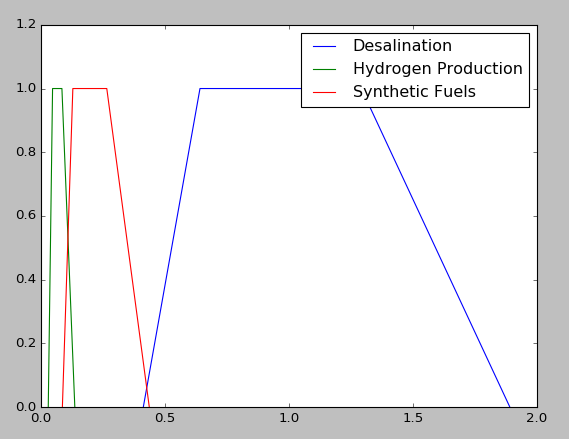
\includegraphics[width=0.5\textwidth]{membership.PNG}
\end{figure}


\begin{table}[h!]
\centering
\caption{AHP Survey answers for determining the relative importance of different criteria}
\label{my-label}
\begin{tabular}{|l|l|l|l|l|l|}
\hline
\begin{tabular}[c]{@{}l@{}}Pairwise \\ Criteria\end{tabular}                       & 1st Expert       & 2nd Expert       & 3rd Expert & 4th Expert       & 5th Expert       \\ \hline
\begin{tabular}[c]{@{}l@{}}Safety vs \\ Ability to \\ Fluctuate\end{tabular}       & Safety: 6        & Safety: 9        & Safety: 8  & Safety: 6        & Safety: 7        \\ \hline
\begin{tabular}[c]{@{}l@{}}Safety vs \\ Profitability\end{tabular}                 & Safety: 8        & Safety: 8        & Safety: 8  & Equal            & Safety: 7        \\ \hline
\begin{tabular}[c]{@{}l@{}}Ability to \\ Fluctuate\\ vs Profitability\end{tabular} & Profitability: 8 & Profitability: 7 & Equal      & Profitability: 8 & Profitability: 4 \\ \hline
\end{tabular}
\end{table}

\newpage
\section{AHP Conclusion and Future Work}

AHP should be used early in the design and decision making process to determine the best options given a set of criteria. Unlike other systems which can be compared to experimental setups, AHP evaluates systems which cannot have large scale experiments. Given the criteria of safety, ability to fluctuate, and profitability a multi-stage flash distillation system appears to be the best choice in a generic setup when compared with synthetic fuels upgrading and hydrogen production from high temperature steam electrolysis. In future work applying AHP to NRHES configurations, considerations such as access to feedstocks, for example water and hydrocarbons, will likely play a large role in determining the industrial process incorporated. 

 Future work on applying AHP to NRHES would include many more criteria, subcriteria, and alternatives which are important to evaluate on a relative basis.  Criteria such as emissions, a key driver for NRHES, would be important to consider before determining the optimal industrial process for a given industrial park. Other criteria such as likely regulatory barriers and state of development of the industrial process technology would also be valuable to include in future research. 
 
\chapter{Thermal Versus Electrical Coupling}
\label{TvsE}
From the literature review on NRHESs, a notable gap in the current research is modeling the benefits gained from thermally coupling industrial processes as compared to electrically coupling. Thermal coupling refers to the industrial process using the heat directly from the nuclear power plant as opposed to electrical coupling in which the industrial process uses the electricity drawn from the power plant. The major drawback of thermally coupling any industrial process to a nuclear power plant is the increase in complexity and the lack of maturity of experience in the domain. While there are cases of thermal coupling of nuclear power plants internationally; in Norway, Switzerland, Germany, and Canada \cite{Verfondern};  there have never been any nuclear thermal couplings thus far in the United States.  The low level state of development as well as the lack of experimental data in the United States suggest a current lack of data and maturity of experience.  There are concerns surrounding the regulatory oversight with a thermally coupled NRHES and whether it falls under the \ac{nrc}'s umbrella. The efficiency benefits would have to be greater than the costs associated with thermal coupling and co-location.  An exergy analysis of both the electrically coupled and thermally coupled industrial processes provides a quantitative measure of the thermodynamic benefits of thermally coupling. As the fuzzy AHP analysis concluded that the optimal industrial process; given the requirements of safety, ability to fluctuate, and profitability; is desalination, the exergy evaluation will focus on two desalination systems.  The thermally coupled system in this analysis is \ac{msf} distillation which will be compared to an electrically coupled \ac{ro} system.

\section{Research Motivation}

There are two primary motivations for the exergy analysis done below.  Initially, the motivation behind this research was to demonstrate the potential costs and benefits of thermally coupling desalination systems to nuclear power plants in a NRHES configuration.  This is still a primary motivation behind the research.  The second motivation came from analyzing the potential nuclear power plants to couple the desalination system. \ac{pvgs} is evaluating the potential benefits of installing an electrically coupled reverse osmosis desalination system.  The RO system will both allow Palo Verde to fluctuate the amount of electricity sent to the electric grid as well as to generate water to first meet the power plant's own water requirements as well as increase the water resources available for communities in the surrounding region. 

Arizona, due to the high penetration of solar in the state, is an ideal setting to try a NRHES. Arizona has been a leader in implementing solar electricity. In 2013, Arizona produced 23.4\% of all US solar generation and 1.9\% of the electricity in Arizona.  In 2016, solar in Arizona produced 3.4\% of the total electricity for the state. The state also has a renewable portfolio standard requiring 15\% renewable energy by 2025 from regulated utilities\cite{DSIRE2017}. With the penetration of solar in the state, other sources of generation are going to need to be more flexible.  

The Palo Verde generating station generates the most electricity of any power plant in the entire United States. In January 2018, Palo Verde produced 36.37\% of Arizona's power\cite{eia2018}.  As such a large contributor to the grid, Palo Verde fluctuating could counterbalance the large shifts in solar power generated during the day and unavailable in the evening and at night. Palo Verde has a zero discharge water cycle.  Zero discharge means unlike most nuclear power plants that release heated water into a body of water, all of the water at Palo Verde either stays at the power plant forever or is evaporated from the evaporation ponds or the cooling towers.  The power plant uses waste water from Phoenix's 91st avenue treatment facility and Tolleson's facility. While at the time of Palo Verde's initial operation, 1986, the treated waste water was not worth very much, with the increasing unavailability of water and population growth in Arizona, the water has become more valuable.  Arizona has significant amounts of brackish groundwater which could be pumped up from underground aquifers and used in place of the treated waste water currently in use at Palo Verde. The general composition of Arizona's brackish groundwater can be seen in Table\ref{ArizonaWater} below.  

\begin{table}[h!]
\centering
\caption{The Components of Briny Groundwater in Central Arizona Centerra Well from \cite{USBureauofReclamation2006}}
\label{ArizonaWater}
\begin{tabular}{|l|l|}
\hline
\textbf{Material}                                                & \textbf{Mole Percent} \\ \hline
Calcium  & 7.32E-3     \\ \hline
Magnesium & 5.11E-3      \\ \hline 
Sodium & 3.24E-2\\ \hline
Sulfate & 9.47E-3 \\ \hline
Barium & 5.25E-6 \\ \hline
Nitrate & 5.20E-4 \\ \hline
Flouride & 6.64E-5 \\ \hline
Arsenic & 7.21E-8 \\ \hline
Water                                                      & 99.9         \\ \hline
\end{tabular}
\end{table}

Palo Verde is pursuing a desalination facility in order to ensure a reliable and cost effective source of water for the power plant while also wanting to ensure the surrounding communities have sufficient water to grow. While Palo Verde is focused on an electrically coupled reverse osmosis system, it is worth knowing what kind of water output would be expected from a thermally coupled system for future plants interested in pursuing desalination and water purification. Palo Verde is pursuing reverse osmosis due to the facility having six separate owners. \ac{aps} is the group considering the reverse osmosis system.  As APS owns about 30\% of the facility, that means it owns about 30\% of the load generated from the facility (about 1200 MW depending on the temperature). APS can thus allocate as much of the electrical load it owns to the reverse osmosis system in order to fluctuate the electric load it is selling to the grid as well as to ensure lower costs of water for the power plant. Even if using waste heat, thermally coupling to a reactor would impact the power cycle of the plant, as discussed in the results below. Thus in order to avoid the complications of determining the technical as well as policy implications of thermally coupling with six owners, it is much simpler for APS to pursue an exclusively electrically coupled system.  Palo Verde demonstrates the restrictions imposed by the costs of increased complexity of thermally coupling.  


\section{Exergy Analysis Background}
Exergy describes the useful energy in a system for generating work. From Newton's first and second laws of thermodynamics, it is clear that not all the energy generated in a system can be converted into usable work.  The first law describes how energy can not be created or destroyed, it can only be converted into a different form.  For example the chemical combustion in a fire producing heat and light. The second law describes the creation of entropy in a system. Entropy is often thought of as the amount of randomness in a system.  Having disorder or randomness in a system requires energy that cannot then be used to generate work. Some energy always goes towards the entropy in the system, making it unusable for doing work. Exergy, also known as the availability, describes the energy available in the system for doing work. Exergy has the same units as energy, most commonly Joules. 

Exergy can be a more descriptive metric than the energy loss as it describes how close a system is to being the ideal design with the least physical possible energy losses across the system. In order to determine the maximum possible energy efficiency of a power cycle requires finding the Carnot efficiency $\eta_{Carnot}=1-\frac{T_0}{T}$.  It is physically impossible for the Carnot efficiency to equal 100\%, which would be a perpetual motion machine.  There will always be losses in the system to maintaining the entropy in the system. The exergy efficiency determines of the energy available to do work, how effective is the cycle design to extracting all of that available energy.  The exergetic efficiency concept can be applied to all of the various components involved in the coupling of a Nuclear Renewable Hybrid Energy system. The exergy analysis can then be combined with an economic analysis determining where exergy losses are most costly. For this project, the components in the exergetic analysis will be applied to include the components modeled in Palo Verde's Rankine Power Cycle as well as the water purification systems.

In an ideal, reversible process, there is no exergy loss or entropy generated. Reversible processes are rightly named as these ideal processes would be able to be restored to their initial state without any external work added to the system. While there are no processes that are fully reversible in reality, an example if possible would be electric flow through a zero resistance material or movement on a fractionless plane. Irreversible processes increase the entropy in the system thereby destroying some of the exergy in the system. Finding whee there is exergy destruction in a system can help indicate where losses are occurring. By applying an economic exergy analysis, the system can be optimized so that the exergy losses are done in the most valuable way possible.
%I need to include the exergy destroyed in the power cycle 
%Do a parametric study including the temperature of the input water
%See if I can easily include solar generation data in the demand data
%Maybe include generator heat losses?

% * <eredfoot@gmail.com> 2018-05-24T16:16:32.855Z:
%  
% Describe why second law efficiency is important. Give a better definition of exergy, maybe discuss perpetual motion machine.
% 
% ^.

The basic mass exergy equation of a system is\cite{moran2010fundamentals}:

\begin{equation}
\triangle X=(U-U_0)+p_0(V-V_0)-T_0(S-S_0)+KE+PE
\end{equation}
\\
Where X is the exergy of the system, U is the internal energy of the system, $p_0$ is the initial pressure of the system, $V$ is the volume of the system, $T_0$ is the initial temperature given in Kelvin, S is the entropy of the system, and KE and PE are the kinetic energy and potential energy. The units for exergy are the same as those for energy. The specific exergy of the system, or the exergy of the system not including the mass is displayed as e.  To find the specific exergy of the system, each of the elements in the equation are divided through by the mass. Specific thermodynamic properties differ from mass thermodynamic properties in that the specific values are characteristics of the materials regardless of mass. The resulting equation for internal exergy is:
\begin{equation}
\label{specificX}
\triangle x=(u-u_0)+p_0(v-v_0)-T_0(s-s_0)+\frac{1}{2}v^2+gh
\end{equation}
\\

Each of the elements now represent the specific values of the system.  For this research, the mass values will be neglected, focusing instead specifically on the internal exergy values. The internal exergy differences thoroughly describe the system.  The mass transfer within either the power cycle or the water purification systems does not provide any extra insight into the relative magnitude of exergy loss in the various components. The kinetic energy term, $\frac{1}{2}v^2$, is generally fairly constant throughout the system and therefore does not need to be taken into consideration.  The potential energy element, $gh$, is negligible throughout the system. The enthalpy, h, of a system, or the total heat content of the system, is equivalent to the specific internal energy plus the pressure times the change in specific volume.  Put mathematically:

\begin{equation}
\triangle h=(u-u_0)+p_0(v-v_0)
\end{equation}

Including enthalpy in the place of the first two elements in \ref{specificX} as well as removing the last two elements leaves the specific exergy equation as simply:

\begin{equation}
\triangle x=(h-h_0)-T_0(s-s_0)
\end{equation}

%The second law of thermodynamics, as defined by the Kelvin-Planck statement is
%\begin{quotation}
%It is impossible for any system to operate in a thermodynamic cycle and deliver a net amount of energy by work to its surroundings while receiving energy by heat transfer from a single thermal reservoir \cite{moran2010fundamentals}.
%\end{quotation} 
%In other words, energy cannot simply be put into a system and work taken out of the system. In every thermodynamic cycle, there has to be some heat ejected into a cold reservoir.
 

\subsection{Relevant Exergy Analysis Research}
  Boldon et. al. has already performed an initial exergy analysis on a \ac{nrhes}, assuming a \ac{smrs}\cite{Boldon}. Boldon et. al. discusses the value of combining exergy and economics to analyze costs associated with exergetic losses.  Boldon et. al. analyzes a steady state system providing a constant grid output of 245 MWe.  The nuclear plant is both thermally and electrically coupled to a High Temperature Steam Electrolysis industrial process. After performing the thermodynamic exergy analysis, Boldon et. al. incorporates costs of resources and operations thereby able to assign a unit exergetic cost to each of the components in the system. This exergy analysis differs in focusing on a current large nuclear power plant, focusing on water purification methods, and including a quasi dynamic approach.  While the value of the electricity and water will be taken into account, the products of the system will dictate the \$/exergy loss as opposed to the costs of the system. In order to include a quasi dynamic approach, both the MSF and RO systems will be evaluated based off of both the optimal \$/exergy costs as well as taking into consideration the load following capabilities valuable to \ac{aps}. 
  
 An exergetic analysis of the Kalundborg industrial ecosystem evaluates the streams going into and out of the Asnaes power plant \cite{Valero2012}.  Valero et. al. contrast the exergy of the coupled system with an uncoupled system. As can be seen in figure \ref{Kalendburg} below, the Kalundborg industrial ecosystem is comprised of the Statoil refinery, the Asnaes coal power plant, the Novo Group pharmaceutical company, district heating for the local people, the Gyproc plasterboard manufacturer, as well as a fish farm, and  the Aalborg Portland cement company. The major exergetic gains for the system come from sharing the process heat from the natural gas, the district heating, heating the fish farm, and using clinker (a coal plant byproduct) to produce cement \cite{Valero2012}. The overall reduction in irreversibilities annually from coupling the systems at Kalundborg amounts to approximately 1476 GWh/year, the equivalent of the annual production of a 170.235 MW power plant. From the Kalundborg example, comparing the exergy of a coupled system with the separate industrial processes provides great insight into the thermodynamic and economic benefits of co-locating processes.

\begin{figure*}
\centering
\label{Kalendburg}
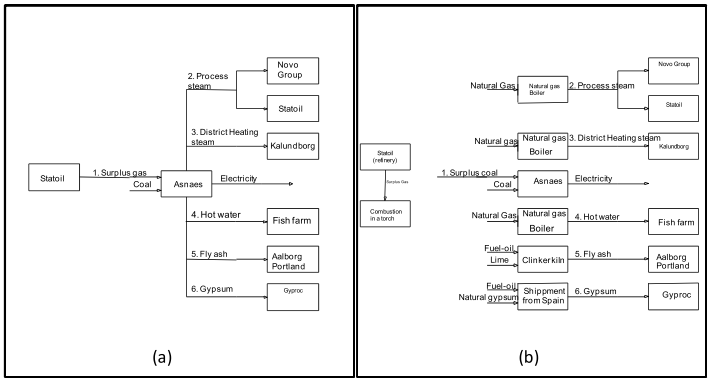
\includegraphics[width=.7\textwidth]{kalundborg_cases.PNG}
\caption{\small \sl This figure displays the two cases evaluated in Valero et. al. Figure a shows the industrial ecosystem in the current coupled form. Figure b shows the second case where there is no coupling.}
\end{figure*}

 
\subsection{Multi-Stage Flash Distillation}
As the NRHES evaluated for this thesis includes a \ac{msf} distillation system, I will include a brief review of a previous MSF distillation exergy analysis. Kahraman et. al. performed an exergy analysis on a large MSF plant \cite{Kahraman2005}.  \ac{msf} distillation only requires heat at about 100 degrees Celsius, making it possible to use high temperature waste heat from a nuclear power plant to desalinate or purify the water. In general, the waste heat coming from a nuclear power plant is significantly below 100\degree C, thus extra heat would need to be sent to the environment, in this case the MSF process, in order to use the waste heat from the reactor. The same processes, RO and MSF, can be used for both water purification and desalination, so the terms can be used fairly interchangeably. In the case of Palo Verde, the system is a water purification system for brackish groundwater. In the exergy analysis, Kahraman et. al. takes the temperature of the salinated water to be the dead state, making the initial exergy zero. Similarly in the exergy analysis done in this thesis, the dead state is taken as the temperature of the water intake. Kahraman et. al.'s exergy analysis includes finding the exergy of the heat exchanger, of four pumps in the system, as well as the difference in exergies between the incoming water and the exiting stream. 

Figure \ref{MSF_x} displays where exergy was destroyed in the MSF system. Clearly the majority, 77.7\%, of the exergy was destroyed in the MSF distillation system itself. Other sources of irreversibilities include the inefficiencies and losses due to the pumps and heat exchangers as well as the final release of the waste brine water to the environment. The exergy destroyed in the MSF system went to a process which produced a valuable product.  The other sources of exergy destruction are strictly physically necessary losses with no economic benefits. In the economic exergy study done in this thesis, the exergy destruction will be evaluated based on its economic value.  Both generating pure water in the MSF system as well as producing electricity result in exergy destruction.

MSF is the most common thermal desalination system. In an MSF system, salt water or brackish water is flash evaporated, then condensed repeatedly in order to remove unwanted particulates. As can be seen in figure \ref{salinity}, Brackish water has more salinity or impurities than fresh water, but not as much as sea water. MSF is able to produce clean water in large quantities, with plants in Saudi Arabia and the United Arab Emirates having capacities of 600,000-880,000 $m^3/day$ \cite{El-Dessouky2016}. The general idea of how an MSF system works is sea water or briny water is passed through a series of chambers, each with successively lower temperature and pressure.  The water is quickly flashed, or vaporized.  The water, without the brine, is then condensed forming freshwater.  There are a wide range of stages, depending on the concentration of the feedwater brine and the desired state of purity for the freshwater. Standard sizes for fairly large MSF arrays come in the form of 21-50 stages. Generally, MSF distillation systems are well developed technology used for high capacity desalination systems.
\begin{figure*}[h!]
\centering
\label{salinity}
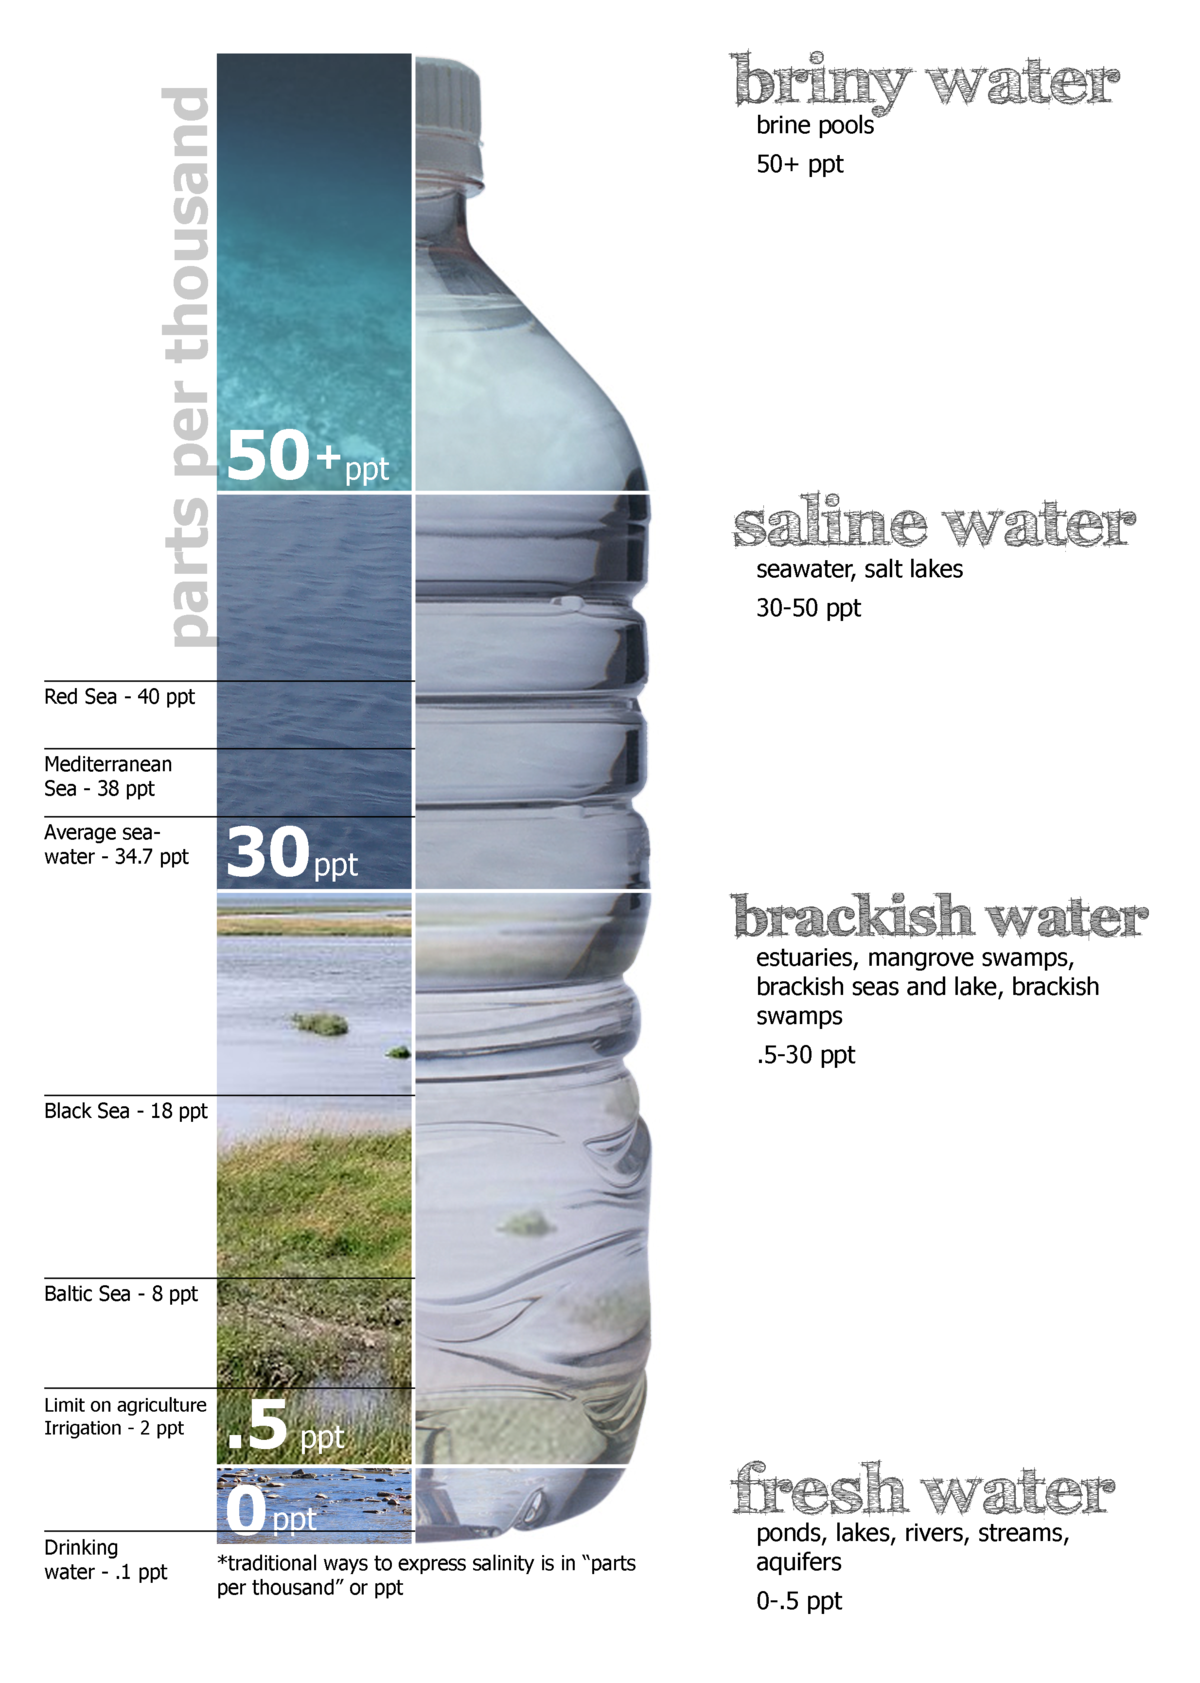
\includegraphics[width=.25\textwidth]{Water_salinity_diagram.png}
\caption{\small \sl This figure displays the differences between different water qualities}
\end{figure*}


In a multi-stage flash system, it is important to keep the temperature relatively low, no greater than 120 \degree C in order to minimize fouling. Fouling and scaling are serious considerations for MSF systems.  Generally, fouling refers to the unwanted deposition of compounds or organic substances on the surface of a host material (membrane, heat exchanger, condenser, etc)\cite{Khayet2016}. In \cite{El-Dessouky2016} the twelve case studies range from 95 \degree C to 105 \degree C. For a more complete range of possible temperatures, this research will analyze temperatures from 80 \degree C to 120 \degree C. The research will seek to optimize the value of the energy throughout the power cycle and industrial process.


\begin{figure*}[h!]
\centering
\label{MSF_x}
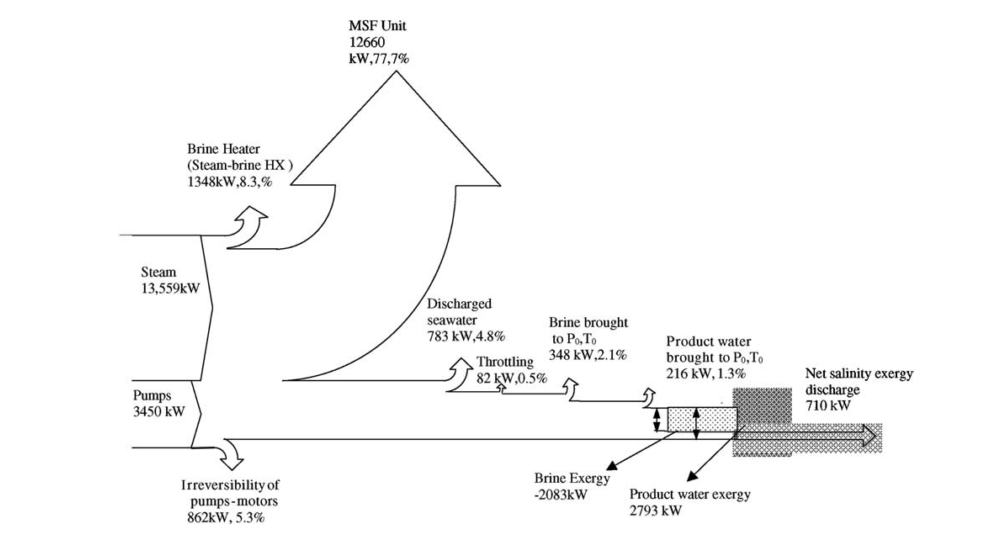
\includegraphics[width=.4\textwidth]{MSF_exergy.PNG}
\caption{\small \sl The Multi-Stage Flash exergy analysis diagram showing where exergy is lost in the system from \cite{Kahraman2005}}
\centering
\end{figure*}

\subsection{Reverse Osmosis}

Reverse osmosis is a type of electrically driven membrane desalination or filtration process. It is able to remove tiny particles of sizes ranging down to 50-200 daltons \cite{Pangarkar2011}. It has relatively high applied pressure values ranging between 1-5 MPa. In general the reverse osmosis system works due to the osmotic pressure differences between salt water/briny water and pure water.  Salt water or briny water is forced through membranes under pressure, separating the feedwater into a pure water stream and a stream with a high concentration of impurities.  About 48\% of reverse osmosis systems are used with brackish water \cite{Pangarkar2011}. 

\section{Methodology}
 The exergy analysis done here will assume a simplified model of the Palo Verde Rankine power cycle and compare a process heat MSF distillation system to a RO system.  First, I will evaluate the \$/exergy cost of a MSF system using the process heat from a nuclear power plant. Then I will look at the exergy costs of the RO system. An exergy analysis really evaluates where there are irreversibilities in a system. In order to show the irreversibilities in the system, I will evaluate the exergy destroyed across each of the subsystems.  With the power cycle, the subsystems include the turbines, the heat exchangers, and the pumps.  The exergy change across the condenser is taken to be the exergy destroyed in order to purify the brackish groundwater. While there is some exergy left in the brackish waste water released to the environment, the exergy destroyed through the condenser provides a general idea of how much exergy was required in the MSF system. In the case of the RO system, the exergy lost in the condenser is part of the exergy loss required for the electricity generation. The exergy losses in the RO system come strictly from the exergy destroyed in the pumps. 
 
The economic values for the system will come from the value of the electricity generated plus the value of the water generated.  The 
 
%Add a big discussion of why I took the exergy difference across the flow to the condenser and the flow from the condenser
 
The system will be modeled using the Aspen HYSYS software.  The power cycle will initially be a simplified version of the Palo Verde Power cycle.  Since the goal in this research is to evaluate the differences in the water purification systems, not the exergy losses in the power cycle, the power cycle model primarily serves to demonstrate how thermally coupling a system impacts the system as a whole.

\subsection{Aspen HYSYS}

Aspen HYSYS is a process simulation software used primarily by the oil and gas industry. In general, process simulation software calculates material and energy balances for a whole plant or process unit. Process simulation software can be used to size the various components in a system for the desired outcome in terms of quality and quantity of product. Aspen HYSYS calculates heat and mass balances, thermodynamic data and equilibrium conditions, sizes equipment, and can do economic optimization and dynamic simulation \cite{Oi2017}. In this model, Aspen HYSYS calculates the overall thermodynamic and mass flow values of the Palo Verde Power Cycle as well as the multistage flash distillation process. The thermodynamic values, such as enthalpy, entropy, temperature, and pressure can then be used to determine the exergy of the system using a User Variable in the system. 

First, I built a model of the Palo Verde power cycle using Aspen HYSYS and coupled it to both a MSF and RO water purification systems. Then, I calculated the \$/exergies in the power cycle and the water purification system using a combination of user variables within Aspen HYSYS as well as spreadsheet calculations, as can be seen in Appendix B. Then, after finding the exergy values, I adjusted the temperature of the water sent to the heat exchanger with the MSF system, initially sent using waste heat, then using process heat.  Waste heat is the heat from a power cycle that would no matter what be released to the environment. 

In order to do an economic analysis, evaluating the \$/exergy, requires knowing the amount of product sold as well as the value of the product. The cost of water for Palo Verde in 2018 is \$130.00 per acre-foot, which comes out to about \$0.105 per cubic meter of water \cite{Brown2018}. The best value I could find for the wholesale value of Palo Verde's electricity is from 2007 at 6.33 cents per kW-h, which is equal to about 8 cents per kW-h including inflation. The actual value of the electricity fluctuates over a day depending on the supply of electricity.  In Arizona's case, the value of the electricity over the course of a day is largely dependent on the amount of solar power on the grid. The fluctuation in power demand for \ac{APS} will be taken into consideration using \ac{raven} to generate demand data for a generic day in each season.  

\subsection{Fluctuating Electricity Output}

In order to be considered by \ac{nerc} a regulating and supplemental reserve of electricity requires non spinning reserve source being able to ramp to full capacity within ten minutes \cite{NERC2014}. NPPs traditionally are unable to fulfill a role as regulating or supplemental reserve because of the inability to ramp to full power quickly.  With a MSF system, the NPP still may be unable to switch the process heat fast enough to meet the NERC's definition. The European Utility Requirements require a NPP to be capable of daily load cycling operation between 50\% and 100\% . The European pressurized water reactor has to satisfy maneuverability requirements including being able to have planned variations in energy output between 25\% and 100\% \cite{NEA2011}. Thus for this research, the MSF process heat model will be evaluated at 25\%, 50\%, 75\%, and 100\% of the heat load from the reactor. Looking at 25\% integrals will give some notion of the relationship between the heat sent to the MSF system and the amount of water collected from the system.

\subsection{Drinking Water Standards}
There are some standards which need to be met when modeling both the water purification system as well as the Palo Verde power cycle.  The main consideration for the water purification system, especially if planning on selling the water to the public, is that the water must meet the standards set out in the Safe Drinking Water Act of 1974. While commercial nuclear power plants dedicate a lot of resources to water chemistry and have very high standards for the water used in the plant, the standard used for this research will be that set for public consumption. Below is a discussion of both the standards as well as the current composition of briny groundwater in Arizona. 

The Safe Drinking Water Act of 1974 gives the \ac{epa} the authority to determine safe drinking water standards. The EPA sets standards on over ninety contaminants in drinking water. The drinking water contaminants fall into the broad categories of microorganisms, disinfection byproducts, disinfectants, inorganic chemicals, organic chemicals, and radionuclides \cite{USEPA}. The components found in Arizona groundwater can be found in table \ref{ArizonaWater}.  None of the components found in Arizona groundwater are regulated by the Safe Drinking Water Act or are covered by the EPA's secondary drinking water standards\cite{USEPA}. The only overlap between the contaminants regulated by the EPA for taste and aesthetic concerns and those found in Arizona groundwater is maintaining the total dissolved solids at 500 mg/L or below. For this research, the water is assumed to be comprised of a more brackish composition than that found in table \ref{ArizonaWater}.The contaminants have been increased nine fold in the composition used in the Aspen HYSYS model as can be seen in table \ref{ModelComp}.  In some cases, there were not the independent materials that were found in the brackish ground water available in the Aspen library.  Thus I combined certain molecules, such as sodium sulfate and sodium nitrate to most closely match the composition found in the groundwater.  By combining these molecules, there may be some difference in the overall composition and the energy it takes to remove the particulates.  The end product is pure water.

\begin{table}[h!]
\centering
\caption{Mole Composition of Brackish Groundwater Assumed in Aspen-HYSYS model}
\label{ModelComp}
\begin{tabular}{|l|l|}
\hline
\multicolumn{1}{|c|}{\textbf{Material}}                   & \multicolumn{1}{c|}{\textbf{Mole Percent}} \\ \hline
Calcium & 1.3E-1 \\ \hline
Magnesium  & 9E-2\\ \hline
Sodium  & 5E-1 \\ \hline
Sodium-Sulfate & 1.7E-1 \\ \hline
Sodium-Nitrate & 9E-2 \\ \hline
Barium & 1E-2 \\ \hline
Water & 99.0  \\ \hline
\end{tabular}
\end{table}

\section{Palo Verde Power Cycle}

Much of the information of the design and functioning of Palo Verde's power cycle can be found in the \ac{ufsar} made publicly available for all nuclear power plants by the \ac{nrc}. Initially, this exergy analysis will model a very basic Rankine cycle with only two turbines. As the exergy analysis for this system is not on the high performing functionality of the turbines or pumps associated with the power cycle, but rather with how the different water purification systems impact the exergy of the cycle, it is not so important to do a completely representational model of the power cycle. 

Some of the key values taken from Palo Verde's \ac{ufsar} are displayed in tables \ref{coreVales} and \ref{PowerValues}.  The key difference between the model values and the Main Steam Flow Power Cycle Values is the mass flow is significantly less for the model 1616 $\frac{kg}{s}$ as opposed to 2200 $\frac{kg}{s}$. The mass flow value is solved for in the model.  Since not all of the components are included in the model, it is reasonable that there is a lower mass flow calculated.%Explain why this makes sense

%Discuss difference in condenser values, maybe change pressure in the model. Figure out the general pressure what is introduced to an MSF system at

%Make a table of the model values for each of theses systems to compare to

\begin{table}[h!]
\centering
\caption{Palo Verde Reactor Core Thermohydraulic Values}
\label{coreValues}
\begin{tabular}{|l|l|l|}
\hline
\textbf{Reactor Core Values} & \textbf{Value Given in FSAR} & \textbf{Units in Model}        \\ \hline
Reactor Outlet Temperature   & 653 \degree F & 345 \degree C   \\ \hline
Reactor Inlet Temperature    & 568 \degree F & 297.8 \degree C \\ \hline
Mass Flow                    & $164.0x10^6\frac{lb}{hr}$    & $20663.6\frac{kg}{s}$          \\ \hline
Pressure                     & 2250 psia                    & 15.513 MPa                     \\ \hline
Power Generation             & 3800 MWt                     & 3800 MWt                       \\ \hline
\end{tabular}
\end{table}

\begin{table}[h!]
\centering
\caption{Palo Verde Main Steam Flow Power Cycle}
\label{PowerValues}
\begin{tabular}{|l|l|l|}
\hline
\textbf{Power Cycle Values} & \textbf{Value Given in FSAR}  & \textbf{Units in Model}          \\ \hline
Steam Temperature at HX     & 552.9 \degree F                & 289.4 \degree C                   \\ \hline
Maximum Quality             & 0.25                          & 0.25                             \\ \hline
Mass Flow                   & $17.2-18.1x10^6\frac{lb}{hr}$ & $2154.56-2280.56 \frac{kg}{sec}$ \\ \hline
Pressure                    & 1070 psia                     & 7.377 MPa                        \\ \hline
Power Generation            & 3800 MWt                      & 3800                             \\ \hline
\end{tabular}
\end{table}

\begin{table}[h!]
\centering
\caption{Palo Verde Main Condenser Values}
\label{Condenser}
\begin{tabular}{|l|l|l|}
\hline
\textbf{Main Condenser Values}                                                       & \textbf{Value Given in FSAR}       & \textbf{Units in Model}          \\ \hline
Feedwater temperature                                                                & 450 degree F                       & 232.22  degree C                 \\ \hline
Total condenser duty                                                                 & $9.04x10^9\frac{Btu}{hr}$          & 2649.36 MW                       \\ \hline
\begin{tabular}[c]{@{}l@{}}Circulating water design\\ flow to condenser\end{tabular} & $560,000\frac{gal}{min}$           & $4233.53 \frac{kg}{s}$           \\ \hline
\begin{tabular}[c]{@{}l@{}}Exhaust Steam to \\ Condenser\end{tabular}                & $9,303,000-9,361,830\frac{lb}{hr}$ & $2154.56-2280.56 \frac{kg}{sec}$ \\ \hline
Pressure                                                                             & 3.5 in.Hg abs                      & 11.8524 kPa                      \\ \hline
\end{tabular}
\end{table}




%Do a calculation to show what percent of Palo Verde's water the system is able to contribute

\subsection{Assumptions}

Given the information above, the assumptions for all of the the Aspen HYSYS models are:
\begin{enumerate}
\item The temperature of the brackish groundwater entering the system is 76 \degree F or 24.44 \degree C. This is the low end of the temperature range for the water currently entering the system. While groundwater would be colder, it likely would need to sit in a pool above ground and would heat up. The assumption of the water being at the low end of what currently flows through the condenser allows an analysis of both using the groundwater as well as allows for a fair comparison of the MSF and RO systems using the most realistic value for both. 
\item There are twenty one stages in the MSF distillation system \cite{Bodalal2010} 
\item The reactor power is 3800 MWth
\item The temperatures for the MSF distillation unit range from 80 \degree C to 120 \degree C
\item The composition of the water is what is shown in \ref{ArizonaWater}
\item There is a 2\% pressure loss across all heat exchangers
\item The turbines in the Palo Verde power cycle have a 90\% adiabatic efficiency
\item The pumps have a 90\% adiabatic efficiency.
\item The fluid package used for the power cycle was Peng-Robinson.
%Explain what this means
\item The fluid package used for the brackish water was Electrolyte NRTL.
%Explain what this means
\item The power cycle is much simplified in order to show the clear impacts of the different water purification techniques as opposed to emphasizing the power cycle itself.
\end{enumerate}

The assumptions for the MSF Aspen HYSYS models are:

\begin{enumerate}
\item The mass flow through the distillation system is the dependent variable while the temperature of the water sent to the unit and the pressure generated from the briny water pump are the independent variables for the MSF system.
\item The reactor power and electricity produced are independent variables.
\item The temperature of the water sent to the condenser is an independent variable.
\item The pump power is a dependent variable.
\item The electric power generated is the independent variable.
\item The amount of water generated is the dependent variable.
\item The temperature of the water sent to the condenser is .1\degree C greater than the input temperature to the MSF distillation column
\end{enumerate}

The assumptions for the RO Aspen HYSYS model are:

\begin{enumerate}
\item The efficiency of the pumps ranged from 70\% to 80\% depending on the specifics of the expected pressure and water outflow given by the company 
\end{enumerate}

The economic assumptions for all Aspen HYSYS models are:
\begin{enumerate}
\item The cost of water for Palo Verde Generating Station is \$130 per acre foot \cite{Brown2018}
%Electricity cost is 6.33 per kwh above
\item The wholesale price which Palo Verde can sell water to the grid is \$.08 per kWh.
\end{enumerate}

The simplified Aspen HYSYS model includes one high pressure and two low pressure turbines.  The three separate turbines allow for one of the turbines to seperately be taken offline to send higher temperature water to the MSF system. The thermodynamic values of the system generally are the same as that of the Palo Verde Generating Station.  The mass flow is less at 1616 $\frac{kg}{s}$ as opposed to the 2200 $\frac{kg}{s}$ at the real power plant. As the thermodynamic values taken for this research are specific values, which do not include the mass flow, the findings should be relevant to any mass flow. Overall, while the simplified Palo Verde Power Cycle does not precisely model the actual power plant, it has enough similarities to suggest some trends by the exergy analysis.

In order to find the \$/exergy values, I did the following calculations:

Multiplied the electricity produced by the system in MW by the wholesale electricity price per MWh assumed for this research to be \$80 per MWh:
\begin{equation*}
Electricity\hspace{.2cm} Revenue=MW_{out}*\frac{\$80}{Mwh}=\frac{\$}{hr}
\end{equation*}

Multiplied the water produced by the system by the wholesale value of water to the Palo Verde Generating Station to find the hourly value of the water
\begin{equation*}
\label{water}
Water\hspace{.2cm} Revenue=\frac{m^3_{out}}{hr}*\frac{\$.105}{m^3}=\frac{\$}{hr}
\end{equation*}

To find the cost of the heat added to the distillation system for the lower water temperature studies, I used the hourly value for electricity, multiplied it by the efficiency of the system, then multiplied it by the heat required by the distillation columns.  This is an imperfect calculation, as the heat value is then based on both the efficiency of the cycle and the cost of electricity.  The heat would have to come from a separate source, either through electricity conversion or more direct heat.  The reality is the added expense of thermally coupling several processes would be unrealistic and the cost of the heat would be too high unless the heat is taken directly from the reactor system.  The examples which include a demand for extra heat for the MSF system are really negligible.  They are included in this study to demonstrate the full range of values that research suggests are possible with MSF.  There might be a way to produce less water with the heat sent to the distillation system, but that research is beyond the scope of this project.  The equation used to find the value of the heat added to the MSF distillation system is thus:
\begin{equation*}
Water\hspace{.2cm} Heat \hspace{.2cm} Cost=\frac{\$}{MWh}*Efficiency*Heat \hspace{.2cm}Required  \hspace{.2cm} by  \hspace{.2cm} MSF=\frac{\$}{hr}
\end{equation*}

To find the \$/exergy destroyed:

\begin{equation*}
\frac{\$}{Exergy\hspace{.2cm}destroyed}=\frac{Electricity \hspace{.2cm} Revenue+ Water \hspace{.2cm} Revenue - Water \hspace{.2cm} Heat\hspace{.2cm}Cost}{Total\hspace{.2cm}Exergy\hspace{.2cm}Destroyed}
\end{equation*}

To find the \$/exergy for the water portion of the system:

\begin{equation*}
\frac{\$}{Exergy\hspace{.2cm}Water}=\frac{Water \hspace{.2cm} Revenue - Water \hspace{.2cm} Heat\hspace{.2cm}Cost}{Total\hspace{.2cm}Exergy\hspace{.2cm}Destroyed\hspace{.2cm}Across\hspace{.2cm}Condenser}
\end{equation*}

For the RO system the same equations were used to generate the electric and water revenues. The $\frac{\$}{exergy}$ cost for the reverse osmosis system I calculated as the water revenue-cost of electricity divided by the exergy used across the pumps:

The total exergy destroyed I calculated as:

\begin{equation*}
Exergy\hspace{.2cm}Destroyed = Power\hspace{.2cm}Cycle\hspace{.2cm}Exergy\hspace{.2cm}Destroyed+RO\hspace{.2cm}Pump\hspace{.2cm}Exergy\hspace{.2cm}Destroyed
\end{equation*}

The \$/exergy value for the RO system is:

\begin{equation*}
\frac{\$}{Exergy\hspace{.2cm}Destroyed}=\frac{Electricity \hspace{.2cm} Revenue+ Water \hspace{.2cm} Revenue}{Exergy\hspace{.2cm}Destroyed}
\end{equation*}

The \$/exergy for just the water in the RO system I calculated as:

\begin{equation*}
\frac{\$}{Exergy\hspace{.2cm}Water}=\frac{Number\hspace{.2cm} of \hspace{.2cm}Pumps*\frac{m^3 \hspace{.2cm}water}{hr}*\frac{\$Water}{m^3}}{Total\hspace{.2cm}Exergy\hspace{.2cm}Destroyed\hspace{.2cm}By\hspace{.2cm}Pumps}
\end{equation*}


\section{Results}

There have been different benefits for coupling a water purification facility to one of the reactors at the Palo Verde Generating station discussed through this thesis.  The benefits include providing reliable and reasonably priced water to Palo Verde, fluctuating the electricity output to the grid, and optimizing the value of the exergy lost in the system.  All three of these scenarios have been addressed with the models generated.

\subsection{Water Output}
Annually, Palo Verde uses approximately 75,700 acre feet per year.  To ensure that Palo Verde continues to have sufficient water for operations coming from groundwater resources, the models developed have been used to determine the resources required to meet 20\% of the annual water demand.  Thus, the system needs to be able to produce approximately 15,140 acre feet per year, or 1.728 acre feet, $2131.45 m^3$, per hour if kept running all year. Meeting this minimum demand was not difficult for either the reverse osmosis or the MSF systems.

While the water output will likely fluctuate depending on the electric grid demand, the average output would need to be $2131.45 m^3$ for the system to produce 20\% of the water demand for Palo Verde.

\subsection{Fluctuation}
The ability of a system to fluctuate is of growing significance and value.  As APS implements the required amount of renewable generation, other generation sources will need to change their output to the grid in response. As determined by the RAVEN assessment, shown in Table 4.9, the power shifts currently required due simply to changes in demand are greater than the amount of power APS owns from Palo Verde for all months besides from winter.  If APS chooses to use Palo Verde as a major tool for load following, it would be most helpful to shift most of the load to something besides from the grid for points in the day.  Clearly, as shown in Figures 4.4 and 4.5 the approach between the maximum electric demand and the minimum electric demand is not a sharp drop off at one point in the day, but more of a gradual approach. Thus, it would be helpful to be able to send various loads to the water purification process for different point in the day. In order to do a parametric study of the ability for the RO system and the MSF systems to take the different amounts of load, I evaluated the systems taking 25\%, 50\%, 75\%, and 100\% as discussed in the literature review surrounding the characteristics demanded for load following in the United States and Europe.

While there has been no quantitative study done in this thesis of the ability of the two water purification techniques to start and stop, from the literature it is clear that it is easier for reverse osmosis systems to run in a dynamic fashion.  The MSF systems produce some briny water initially as the heat is allocated to the process.  The RO systems, being essentially a bunch of pumps forcing water through membranes, are able to start and stop and produce the same quality of water.  Both systems are able to start and stop.  In the AHP analysis, desalination ranked highest in ability to fluctuate, while this is an imperfect measure, it does suggest that there is a benefit surrounding ability to fluctuate and desalination.

As can be seen in table \ref{LoadFollow} below, the greatest overall revenue as well as the greatest exergy values overall as well as specifically for the water generation all come when there is more heat being sent to the electricity generation.  The assumption for this data set is that the value of one MWe is \$80.  If the wholesale price per MWe drops below \$0.62 per MWe, the best overall revenue for the heat would come from sending all of the heat to the water production. At times where all or nearly all of the electric demand for a given region is produced by renewables, the price can drop to negative pricing at times.  During this time, the plant would take in more revenue by switching to producing water. Clearly, as can be seen in column 3 of table \ref{LoadFollow}, the facility is producing much more than the $10657.3 \frac{m^3}{hr}$ average hourly water consumption of Palo Verde.   The excess water generated could either be stored or sold to the public. The full results and values found for the load following scenarios can be seen in Appendix B. 

\begin{table}[h!]
\centering
\caption{The load following outcomes using the thermally coupled MSF distillation system at the various load reduction levels required for European reactors as given by \cite{NEA2011}}
\label{LoadFollow}
\begin{tabular}{|l|l|l|l|l|l|l|l|}
\hline
\multicolumn{1}{|c|}{\textbf{\begin{tabular}[c]{@{}c@{}}Load\\  Following\\ Percent \\ Reduction\end{tabular}}} & \multicolumn{1}{c|}{\textbf{\begin{tabular}[c]{@{}c@{}}Input \\ Water\\ Temp\\ (Celsius)\end{tabular}}} & \textbf{\begin{tabular}[c]{@{}l@{}}Volume\\ Flow Out\\ $\frac{m^3}{hr}$\end{tabular}} & \textbf{\begin{tabular}[c]{@{}l@{}}Power\\ MWe\end{tabular}} & \textbf{\begin{tabular}[c]{@{}l@{}}Hourly\\ Water\\ Value\\  (\$/hr)\end{tabular}} & \textbf{\begin{tabular}[c]{@{}l@{}}Hourly \\ Value\\ Electricity\\ (\$/hr)\end{tabular}} & \textbf{\$/exergy} & \textbf{\begin{tabular}[c]{@{}l@{}}\$/exergy\\ Water\end{tabular}} \\ \hline
25\%                                                                                                            & 80                                                                                                      & 17204.0                                                                                        & 923.57                                                       & 1816.74                                                                            & 73,885.59                                                                                & 73.49              & 4.01                                                               \\ \hline
50\%                                                                                                            & 80                                                                                                      & 19136.7                                                                                        & 604.55                                                       & 2020.84                                                                            & 48,363.97                                                                                & 46.50              & 3.23                                                               \\ \hline
75\%                                                                                                            & 80                                                                                                      & 20954.1                                                                                        & 301.01                                                       & 2212.75                                                                            & 24,080.64                                                                                & 24.99              & 2.60                                                               \\ \hline
100\%                                                                                                           & 80                                                                                                      & 22756.7                                                                                        & 0                                                            & 2403.11                                                                            & 0                                                                                        & 2.25               & 2.24                                                               \\ \hline
\end{tabular}
\end{table}

The reverse osmosis fluctuation output follows are shown in the tables below.  For the SW-S pump with a power of 132 kW:

\begin{table}[h!]
\centering
\caption{Exergy Analysis of the IDE-Progreen SW-S 132 kW pump}
\label{SW-S}
\begin{tabular}{|l|l|l|l|l|l|l|l|}
\hline
\multicolumn{1}{|c|}{\textbf{\begin{tabular}[c]{@{}c@{}}Load\\  Following\\ Percent \\ Reduction\end{tabular}}} & \multicolumn{1}{c|}{\textbf{\begin{tabular}[c]{@{}c@{}}Number of\\ Pumps\end{tabular}}} & \multicolumn{1}{c|}{\textbf{\begin{tabular}[c]{@{}c@{}}Input \\ Water\\ Temp\\ (Celsius)\end{tabular}}} & \textbf{\begin{tabular}[c]{@{}l@{}}Volume\\ Flow Out\\ (m\textasciicircum{}3/hr)\end{tabular}} & \textbf{\begin{tabular}[c]{@{}l@{}}Power\\ MWe\end{tabular}} & \textbf{\begin{tabular}[c]{@{}l@{}}Hourly \\ Total\\ Revenue\\ (\$/hr)\end{tabular}} & \textbf{\$/exergy} & \textbf{\begin{tabular}[c]{@{}l@{}}\$/exergy\\ Water\end{tabular}} \\ \hline
25\% & 2280 & 24.44 & 95098.8  & 930.54 & 84428.57   & 3.71 & 0.46 \\ \hline
50\%  & 4560& 24.44 & 190197.6  & 629.58 & 70337.15 & 1.58 & 0.46  \\ \hline
75\%   & 6840 & 24.44   & 569635.2                                                                                       & 328.62                                                       & 86101.3                                                                              & 0.85               & 0.46                                                               \\ \hline
100\% & 9120& 24.44 &  380395.2  & 0  & 42154.3  & 0.48 & 0.46                                                               \\ \hline
\end{tabular}
\end{table}


For the SW-L:

\begin{table}[h!]
\centering
\caption{Exergy Analysis of the IDE-Progreen SW-L 630 kW pump}
\label{SW-L}
\begin{tabular}{|l|l|l|l|l|l|l|l|}
\hline
\multicolumn{1}{|c|}{\textbf{\begin{tabular}[c]{@{}c@{}}Load\\  Following\\ Percent \\ Reduction\end{tabular}}} & \multicolumn{1}{c|}{\textbf{\begin{tabular}[c]{@{}c@{}}Number of\\ Pumps\end{tabular}}} & \multicolumn{1}{c|}{\textbf{\begin{tabular}[c]{@{}c@{}}Input \\ Water\\ Temp\\ (Celsius)\end{tabular}}} & \textbf{\begin{tabular}[c]{@{}l@{}}Volume\\ Flow Out\\ (m\textasciicircum{}3/hr)\end{tabular}} & \textbf{\begin{tabular}[c]{@{}l@{}}Power\\ MWe\end{tabular}} & \textbf{\begin{tabular}[c]{@{}l@{}}Hourly \\ Total\\ Revenue\\ (\$/hr)\end{tabular}} & \textbf{\$/exergy} & \textbf{\begin{tabular}[c]{@{}l@{}}\$/exergy\\ Water\end{tabular}} \\ \hline
25\%                                                                                                            &478 &24.44                                                                                                   & 99567.4                                                                                        & 930.36                                                       & 84428.57                                                                             & 18.01              & 2.84                                                               \\ \hline
50\%                                                                                                            &956 &24.44                                                                                                   & 199134.8                                                                                       & 629.22                                                       & 71246.75                                                                             & 8.49               & 2.84                                                               \\ \hline
75\%                                                                                                            &1434 &24.44                                                                                                   & 298702.2                                                                                       & 328.62                                                       & 86101.3                                                                              & 4.77               & 2.84                                                               \\ \hline
100\%                                                                                                           & 1912&24.44                                                                                                   & 398269.6                                                                                       & 0                                                            & 43973.51                                                                             & 2.79               & 2.84                                                               \\ \hline
\end{tabular}
\end{table}

For the SW-M:

\begin{table}[h!]
\centering
\caption{Exergy Analysis of the IDE-Progreen SW-M 132 kW pump}
\label{SW-M}
\begin{tabular}{|l|l|l|l|l|l|l|l|}
\hline
\multicolumn{1}{|c|}{\textbf{\begin{tabular}[c]{@{}c@{}}Load\\  Following\\ Percent \\ Reduction\end{tabular}}} & \multicolumn{1}{c|}{\textbf{\begin{tabular}[c]{@{}c@{}}Number of\\ Pumps\end{tabular}}} & \multicolumn{1}{c|}{\textbf{\begin{tabular}[c]{@{}c@{}}Input \\ Water\\ Temp\\ (Celsius)\end{tabular}}} & \textbf{\begin{tabular}[c]{@{}l@{}}Volume\\ Flow Out\\ (m\textasciicircum{}3/hr)\end{tabular}} & \textbf{\begin{tabular}[c]{@{}l@{}}Power\\ MWe\end{tabular}} & \textbf{\begin{tabular}[c]{@{}l@{}}Hourly \\ Total\\ Revenue\\ (\$/hr)\end{tabular}} & \textbf{\$/exergy} & \textbf{\begin{tabular}[c]{@{}l@{}}\$/exergy\\ Water\end{tabular}} \\ \hline
25\%                                                                                                            &2280 & 24.44                                                                                                   & 189878.4                                                                                       & 930.54                                                       & 94380.43                                                                             & 8.97               & 2.10                                                               \\ \hline
50\%                                                                                                            &4560 &24.44                                                                                                   & 379756.8                                                                                       & 629.58                                                       & 90240.86                                                                             & 4.51               & 2.10                                                               \\ \hline
75\%                                                                                                            & 6840& 24.44                                                                                                   & 569635.2                                                                                       & 328.62                                                       & 86101.3                                                                              & 2.92               & 2.10                                                               \\ \hline
100\%                                                                                                           &9120 &24.44                                                                                                   & 759513.6                                                                                       & 0                                                            & 81961.73                                                                             & 2.10               & 2.10                                                               \\ \hline
\end{tabular}
\end{table}

\newpage

\subsection{Exergy Optimization}
For the system to make the most money for the amount of exergy destroyed, the MSF system running at 95\degree C has the strongest outcome, given the assumptions built into the model.  The 95 \degree C outcome allows for a lot of water production without adding energy to the distillation columns. The amount of electricity produced is also relatively high with about a 27.2\% efficiency.  

While the exergy loss over the condenser was the least when producing the most electricity, there is substantial exergy loss over each of the turbines.  The exergy destruction in the turbines goes towards making electricity. For the RO system the exergy for the electricity loss plus the exergy destroyed in the pumps is taken into consideration.  Given the quantity of water being pumped to meet the amount of water output by the MSF system, a lot of pumps are required in the RO system.


While temperatures from 80\degree C to 120 \degree C are taken into consideration in the model, the results displayed here display the best outcomes in terms of water produced, revenue, and \$/exergy values. Note that at the higher temperatures for the water entering the distillation columns, there is less mass flow in both the brine and the distillate.  There is less mass flow in general due to less water being able to be heated to 105 \degree C as compared to 80 \degree C.
%Make a table of the best results for the MSF system. Include the temp sent to the condenser, the temp of the water in the distillation columns, the amount of electricity, the amount of water generated, the overall revenue of the system, revenue from water, and the $/exergy values
\begin{table}[h!]
\centering
\caption{Exergy analysis of the MSF system}
\label{MSF-X}
\begin{tabular}{|l|l|l|l|l|l|l|l|}
\hline
\multicolumn{1}{|c|}{\textbf{\begin{tabular}[c]{@{}c@{}}Input\\ Water\\ Temp\\ (C)\end{tabular}}} & \multicolumn{1}{c|}{\textbf{\begin{tabular}[c]{@{}c@{}}Distillation\\ Temp\\ (Celsius)\end{tabular}}} & \textbf{\begin{tabular}[c]{@{}l@{}}Power\\ Cycle\\ Efficiency\end{tabular}} & \textbf{\begin{tabular}[c]{@{}l@{}}Water\\ Generated\\ (m\textasciicircum{}3/hr)\end{tabular}} & \textbf{\begin{tabular}[c]{@{}l@{}}Hourly\\ Water\\ Value\\  (\$/hr)\end{tabular}} & \textbf{\begin{tabular}[c]{@{}l@{}}Hourly\\ Total\\ Revenue\\ (\$/hr)\end{tabular}} & \textbf{\$/exergy} & \textbf{\begin{tabular}[c]{@{}l@{}}\$/exergy\\ Water\end{tabular}} \\ \hline
95                                                                                                & 80                                                                                                    & 27.2\%                                                                      & 16607.06771                                                                                    & 1755.22                                                                            & 84488.69                                                                            & 82.02              & 4.72                                                               \\ \hline
100                                                                                               & 80                                                                                                    & 26.4\%                                                                      & 16801.98762                                                                                    & 1775.82                                                                            & 81908.21                                                                            & 79.51              & 4.49                                                               \\ \hline
105                                                                                               & 105                                                                                                   & 25.5\%                                                                      & 11655.60187                                                                                    & 1231.89                                                                            & 78767.69                                                                            & 76.46              & 2.94                                                               \\ \hline
110                                                                                               & 80                                                                                                    & 24.7\%                                                                      & 17176.15224                                                                                    & 1815.36                                                                            & 76795.08                                                                            & 74.55              & 4.10                                                               \\ \hline
\end{tabular}
\end{table}


%Make a table of the RO system. Include the number of pumps, amount of water generated total revenue, revenue for water, overall exergy values and water specific exergy values.




\begin{table}[h!]
\centering
\caption{Reverse Osmosis Exergy Analysis values}
\label{RO-X}
\begin{tabular}{|l|l|l|l|l|l|l|}
\hline
\multicolumn{1}{|c|}{\textbf{\begin{tabular}[c]{@{}c@{}}Type of\\ Pump\end{tabular}}} & \multicolumn{1}{c|}{\textbf{\begin{tabular}[c]{@{}c@{}}Number of\\ Pumps\end{tabular}}} & \textbf{\begin{tabular}[c]{@{}l@{}}Water\\ Generated\\ (m\textasciicircum{}3/hr)\end{tabular}} & \textbf{\begin{tabular}[c]{@{}l@{}}Hourly\\ Water\\ Value\\  (\$/hr)\end{tabular}} & \textbf{\begin{tabular}[c]{@{}l@{}}Hourly\\ Total\\ Revenue\\ (\$/hr)\end{tabular}} & \textbf{\$/exergy} & \textbf{\begin{tabular}[c]{@{}l@{}}\$/exergy\\ Water\end{tabular}} \\ \hline
SW-S                                                                                  & 52                                                                                      & 2168.92                                                                                        & 227.74                                                                             & 98198.62                                                                            & 64.36              & 0.46                                                               \\ \hline
SW-L                                                                                  & 11                                                                                      & 2291.3                                                                                         & 240.59                                                                             & 98206.19                                                                            & 88.09              & 2.84                                                               \\ \hline
SW-M                                                                                  & 26                                                                                      & 2165.28                                                                                        & 227.35                                                                             & 98472.79                                                                            & 86.51              & 2.10                                                               \\ \hline
\end{tabular}
\end{table}

Table \ref{RO-X} assumes the initial goal of providing, on an hourly averaged scale, 20\% of Palo Verde's water demand. In order to do a more even comparison, the table below displays and RO exergy analysis assuming approximately the same amount of water generated as the highest exergy value system found for the MSF system, the 95 \degree water temperature with the 80\degree distillation temperature shown in row one of \ref{MSF-X}.  

\begin{table}[h!]
\centering
\caption{Reverse Osmosis Exergy Analysis Values Generating similar amounts of water as generated in the MSF system}
\label{RO-H20}
\begin{tabular}{|l|l|l|l|l|l|l|}
\hline
\multicolumn{1}{|c|}{\textbf{\begin{tabular}[c]{@{}c@{}}Type of\\ Pump\end{tabular}}} & \multicolumn{1}{c|}{\textbf{\begin{tabular}[c]{@{}c@{}}Number of\\ Pumps\end{tabular}}} & \textbf{\begin{tabular}[c]{@{}l@{}}Water\\ Generated\\ (m\textasciicircum{}3/hr)\end{tabular}} & \textbf{\begin{tabular}[c]{@{}l@{}}Hourly\\ Water\\ Value\\  (\$/hr)\end{tabular}} & \textbf{\begin{tabular}[c]{@{}l@{}}Hourly\\ Total\\ Revenue\\ (\$/hr)\end{tabular}} & \textbf{\$/exergy} & \textbf{\begin{tabular}[c]{@{}l@{}}\$/exergy\\ Water\end{tabular}} \\ \hline
SW-S                                                                                  & 399                                                                                     & 16642.29                                                                                       & 1727.44                                                                            & 93678.24                                                                            & 19.38              & 0.46                                                               \\ \hline
SW-L                                                                                  & 80                                                                                      & 16664                                                                                          & 1749.72                                                                            & 93957.72                                                                            & 57.07              & 2.84                                                               \\ \hline
SW-M                                                                                  & 200                                                                                     & 16656                                                                                          & 1748.88                                                                            & 95828.88                                                                            & 51.46              & 2.10                                                               \\ \hline
\end{tabular}
\end{table}

From Tables \ref{MSF-X}, \ref{RO-X}, and \ref{RO-H20} it appears that likely the highest \$/exergy value comes from the thermally coupled MSF system, depending on the amount of water desired from the system. From the exergy analysis, it is clear that the \$/exergy value for the water generation is significantly greater when using the thermally coupled MSF system.  This is due to the exergy destruction which occurs in the power cycle in addition to the exergy destruction which occured in the pumps for the RO system.  The MSF system, on the other hand, used exergy that was already being released into the environment, cooling towers and evaporation ponds, in the form of waste heat.  While additional heat was required for the system to produce clean water, there was only so much additional heat required. 

	A quick analysis with the reverse osmosis options found that when the value of the water rose to $\frac{\$0.26}{m^3}$  all three of the pump scenarios included generated water which was worth more than the electricity consumed by the reactor.  Also, if the price of electricity dropped below $\frac{\$33}{MWh}$ the value of the water produced was greater than the value of the electricity consumed for the reverse osmosis systems. A similar analysis for the \ac{msf} system found that when the price of electricity dropped below $\frac{\$8.90}{MWh}$, it was more valuable to have the thermally coupled system at 95\degree C with the distillation at 80\degree C than to use the exergy to generate more electricity. Also, at the $\frac{\$80}{MWh}$ price for electricity, if water rose above $\frac{\$0.95}{m^3}$, it would be more profitable to generate the water at 95 \degree C from the power cycle and 80\degree C entering the distillation system.
    
	One thing that is clear given the average prices assumed at this point is that the greatest amount of revenue between the two purification systems clearly comes from the reverse osmosis system.  The model assumes a much higher value for the electricity than for the water generated.  If trends continue with renewables at times pushing down the price of electricity to close to zero it is likely there will be times when generating water will generate more revenue.  The model also assumes the current purchase price of water, as of 2018, for Palo Verde Generating Station. The predicted price of water is assumed to double by 2025\cite{Brown2018}.  Palo Verde could also sell water to the public at significantly higher prices, resulting in water production profit competing with electricity production profit at times. As water demand increases in the area, and greater amounts of solar generation in particular are added to the grid, the revenue generated by a thermally coupled MSF system could grow to be greater than a strictly electrically coupled RO system. At the moment, assuming average values for water costs and wholesale electricity price, the RO system both brings in significantly greater revenue as well as is much simpler to couple and operate.  


\section{Dynamic Analysis using \ac{raven}}

Through the literature review, this thesis has emphasized the importance of dynamic modeling in analyzing a \ac{nrhes}. Currently, \ac{aps} has about 10\% of the electricity consumed by retail customers coming from renewable energy, primarily solar \cite{ArizonaPublicService2018}.  By 2025, 15\% of all of APS's electricity generation is mandated to come from renewables \cite{UtilitiesDivision}. The increasing penetration of renewables makes a more flexible system more valuable along with the ability to meet variable demand. In order to include a quasi dynamic analysis, \ac{raven} is used to determine the one to two major times in the day there is a major shift in energy demand. In order to determine a standard day, \ac{raven} is used to generate a standard day in winter, spring, summer, and fall in Arizona. The \ac{aps} demand data comes from the \ac{eia} and includes from July 1st, 2015 until May 18th, 2018 as the data the standard day is based off of.  The dates for the beginning and end of each season were pulled from the Farmers' Almanac\cite{Almanac}.

\subsection{Demand Generation Approach}
RAVEN was introduced prior in the discussion surrounding the current NRHES modeling approaches.  As described previously, RAVEN was initially built for probable risk assessment.  It has been used to generate synthetic data for wind demand in prior NRHES modeling as well as to do sensitivity analyses and uncertainty analyses.  For this analysis, RAVEN generates synthetic data of the demand for APS in the various seasons.  Due to the weather changes, consumption of electricity can change greatly.  In the summer, there may be more demand due to air conditioning costs while in the winter, there may be more demand due to heating costs.  As can be seen in Figure 4.5 below, the overall demand for Arizona is greatest in the summer, which likely could be due to air conditioning costs. 

RAVEN uses different \ac{roms} to simplify data in order to first determine general trends, and then to generate new data similar to the input data. RAVEN is used in risk assessment to determine at what point is a system likely to fail. For example, if a lot of data points have been collected on a metal joint failing at various temperature and pressure conditions, RAVEN could be used to find the boundary conditions that result in failure. The process for using RAVEN is to first train the ROM with known data, then to generate new data with similar statistical qualities, such as the mean and the standard deviation. In this research, the input data was the APS demand data for each season from the \ac{eia} from July 1st, 2015 through May 18th, 2018. The generated data came from training a ROM called \ac{arma} on the demand data and then producing new data using the trained ARMA ROM.

ARMA, as the name suggests, is comprised of two parts an autoregressive and a moving average part.  The autoregressive part uses the previous data for the time of day and demand to predict future values for the demand at that time of day. The moving average part includes the error term in the data as a linear combination of current and previous error terms. As can be seen in the raw data graphs below, there are a lot of different demand paths for each of the seasons. The ARMA model used in this research uses a Monte Carlo Sampler.  A Monte Carlo approach generates inputs which it then applies various computations to. In this case, the inputs could be the demand for a given time and the computations could surround the errors associated with that input. The ARMA model is then used to generate 10 different possible demand curves for each of the seasons.  The generated demand curves have very similar means and standard deviation values as those found in the raw data. The ARMA model can thus be used to show general trends found in the demand for each of the seasons.

The graphs in Figure 4.4 show the various daily demand curves that occurred during the referenced period. The raw data curves display the range in possible values throughout the day. Each of the graphs in Figure 4.5 display ten synthetically generated curves that produce a typical day in each season. For spring, graph A, there is low demand in the middle of the day as would be expected for when people are at work. The high electricity demand in the middle of the night may be attributed to industrial consumption combined with many customers having rooftop solar.  Arizona Public Service generates about 500 MW in rooftop solar as well as about 500 MW in large scale solar installations. While APS is one of the two electricity service providers for Phoenix, the rest of its territory is in northern and central Arizona which does not get as hot. Figure \ref{SyntheticAverage} graph d, the winter average, shows two distinct humps.  The first hump peaks at about 4 AM while the second hump peaks at about 4 PM. The high demand at these points could correspond to a combination of when people typically wake up as well as when the sun typically rises. The sun typically rises around 7:00 AM in Tucson in the winter.  At this point, the demand is rapidly decreasing.  A typical change in demand can be determined using the synthetically generated curves. From the synthetically generated curves, the largest demand change can be approximated to include in the analysis of the coupled desalination systems. 

%Figure out why the graphs all show low electric consumption in the middle of the day when it would likely be hottest out

\begin{figure*}[t!]
    \centering

    \begin{subfigure}[b]{\textwidth}
        \centering
        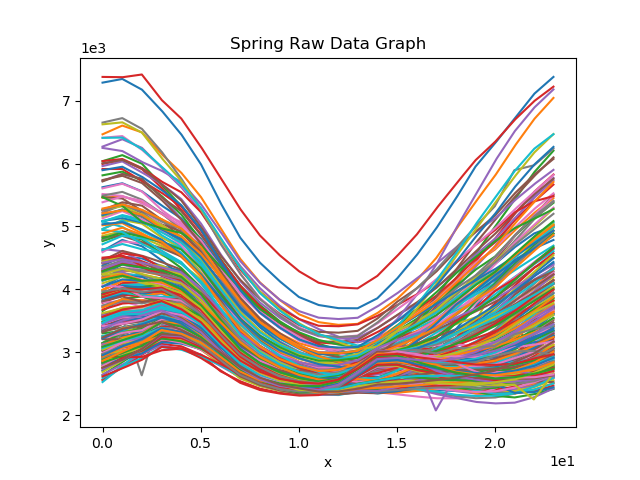
\includegraphics[height=1.8in]{Spring_Raw_Data_Graph_line.png}
        \caption{Raw \ac{aps} Spring Demand Data. x is in hours (the 24 hours in a day). y is APS's electric demand in MWe.}
    \end{subfigure}
     \hfill
    \begin{subfigure}[t]{\textwidth}
        \centering
        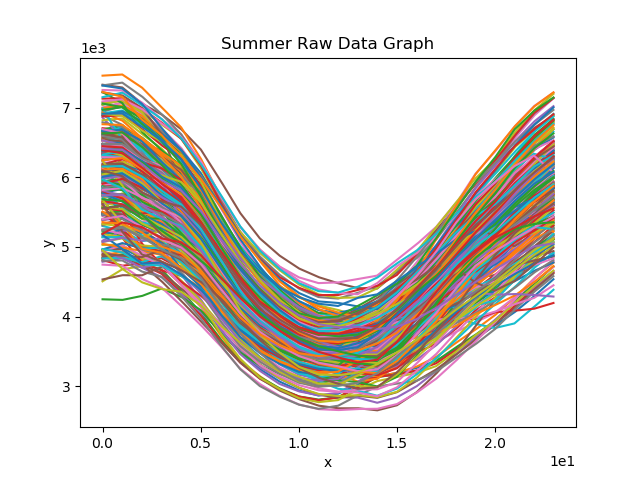
\includegraphics[height=1.8in]{Summer_Raw_Data_Graph_line.png}
        \caption{Raw \ac{aps} Summer Demand Data. x is in hours. y is APS's electric demand in MWe.}
    \end{subfigure}
    \vskip\baselineskip
    \begin{subfigure}[t]{\textwidth}
        \centering
        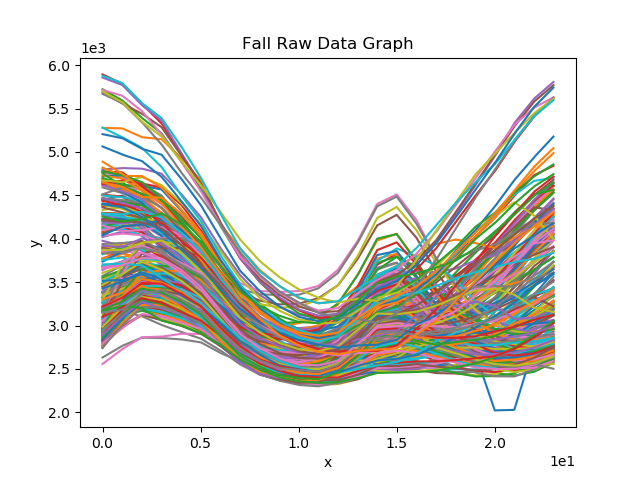
\includegraphics[height=1.8in]{Fall_Raw_Data_Graph_line.png}
        \caption{Raw \ac{aps} Fall Demand Data. x is in hours. y is APS's electric demand in MWe.}
    \end{subfigure}
    \quad
    \begin{subfigure}[t]{0.9\textwidth}
        \centering
        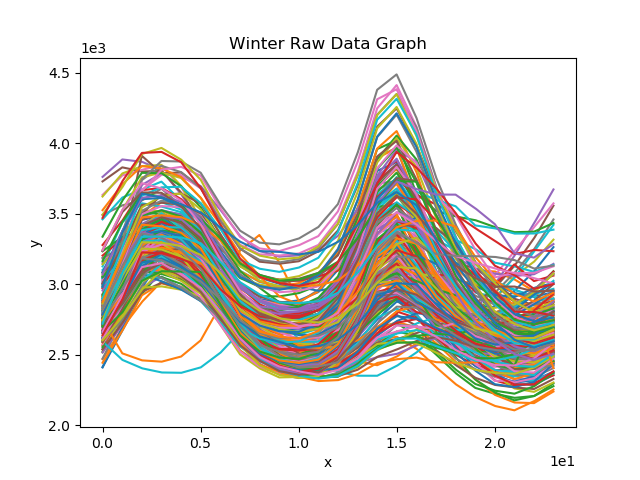
\includegraphics[height=1.8in]{Winter_Raw_Data_Graph_line.png}
        \caption{Raw \ac{aps} Winter Demand Data. x is in hours. y is APS's electric demand in MWe.}
    \end{subfigure}
        \label{RawDemand}
    \caption{Raw Data showing general Arizona Public Service Demand from the EIA from July 1st, 2015 to May 18, 2018}
\end{figure*}

\begin{figure*}[t!]
    \centering
    \label{SyntheticAverage}
    \begin{subfigure}[b]{0.9\textwidth}
        \centering
        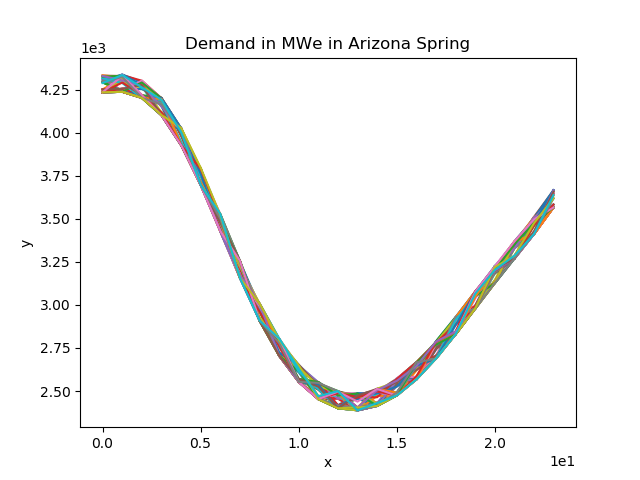
\includegraphics[height=1.8in]{Demand_in_MWe_in_Arizona_Spring_line.png}
        \caption{Spring \ac{aps} Demand Data. x is in hours (the 24 hours in a day). y is APS's electric demand in MWe.}
    \end{subfigure}
     \hfill
    \begin{subfigure}[t]{0.9\textwidth}
        \centering
        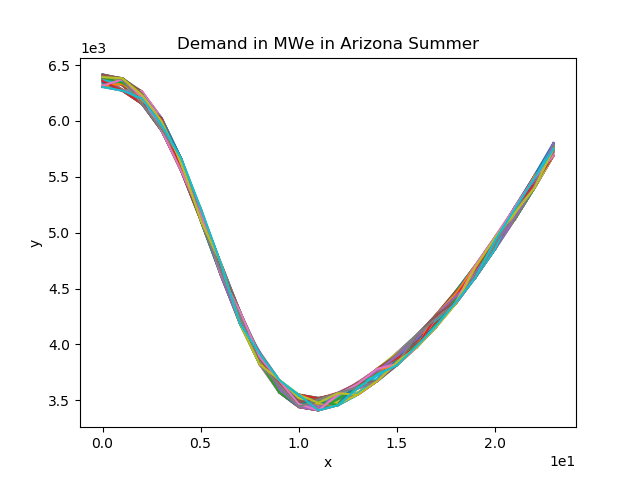
\includegraphics[height=1.8in]{Demand_in_MWe_in_Arizona_Summer_line.png}
        \caption{Synthetic \ac{aps} Summer Demand Data. x is in hours. y is APS's electric demand in MWe.}
    \end{subfigure}
    \vskip\baselineskip
    \begin{subfigure}[t]{0.9\textwidth}
        \centering
        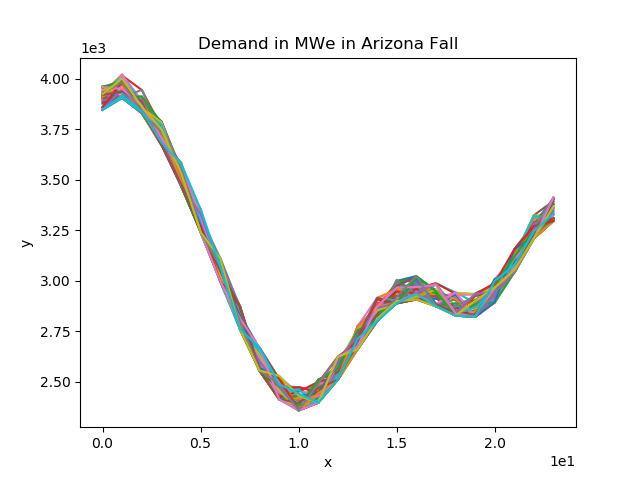
\includegraphics[height=1.8in]{Demand_in_MWe_in_Arizona_Fall_line.png}
        \caption{Synthetic \ac{aps} Fall Demand Data. x is in hours. y is APS's electric demand in MWe.}
    \end{subfigure}
    \quad
    \begin{subfigure}[t]{0.9\textwidth}
        \centering
        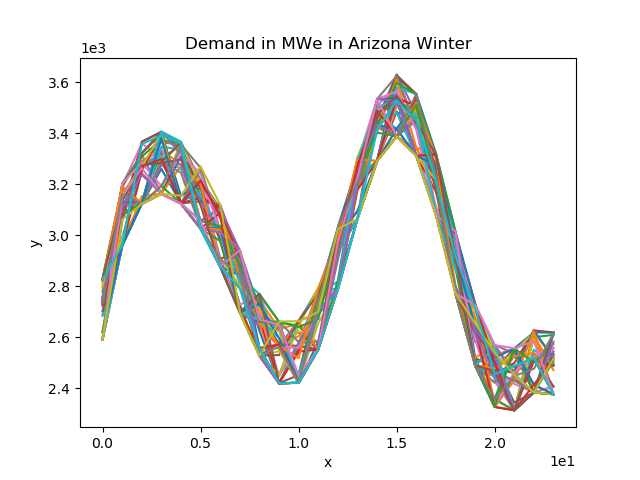
\includegraphics[height=1.8in]{Demand_in_MWe_in_Arizona_Winter_line.png}
        \caption{Synthetic \ac{aps} Winter Demand Data. x is in hours. y is APS's electric demand in MWe.}
    \end{subfigure}
    \caption{Cleaned up Synthetic Data showing general Arizona Public Service Demand}
\end{figure*}

\begin{table}[]
\centering
\caption{Approximate average values for demand change in Arizona over the four seasons}
\label{DemandChange}
\begin{tabular}{|l|l|l|l|l|l|}
\hline
\multicolumn{1}{|c|}{\textbf{Season}} & \multicolumn{1}{c|}{\textbf{\begin{tabular}[c]{@{}l@{}}Peak\\ Demand\\ (MWe)\end{tabular}}} & \textbf{\begin{tabular}[c]{@{}l@{}}Minimum\\ Demand\\ (MWe)\end{tabular}} & \textbf{\begin{tabular}[c]{@{}l@{}}Change in\\ Demand\\ (MWe)\end{tabular}} & \textbf{\begin{tabular}[c]{@{}l@{}}Local\\ Minimums\\ (MWe)\end{tabular}} & \textbf{\begin{tabular}[c]{@{}l@{}}Change in \\ Local\\Demand (MWe)\end{tabular}} \\ \hline
Spring                                & 4300                                      & 2320                                                              & 1980                                                                & N/A                                                               & N/A                                                                        \\ \hline
Summer                                & 6400                                      & 3500                                                              & 2900                                                                & N/A                                                               & N/A                                                                        \\ \hline
Fall                                  & 3900                                      & 2350                                                              & 1550                                                                & 2950                                                              & 950                                                                        \\ \hline
Winter                                & 3500                                      & 2450                                                              & 1050                                                                & 2500                                                              & 1000                                                                       \\ \hline
\end{tabular}
\end{table}

\subsection{Fluctuation Analysis}
As the graphs and table \ref{DemandChange} demonstrate, generally the load change over a day would require all of the electricity being diverted from the APS owned load from Palo Verde.  Since the demand curves drop and increase over several hours typically, the load would need to be shifted to water production in portions over the day if load following just with Palo Verde.  The various exergy and revenue outcomes from the thermally and electrically coupled systems at different rates of load following have already been detailed in tables \ref{LoadFollow}, \ref{SW-S}, \ref{SW-L}, and \ref{SW-M}. The tendency for the demand to shift gradually would suggest a benefit to electrically coupling which does not have thermalhydraulic feedbacks from shifting.

%Discuss thermalhydraulic feedbacks

\chapter{Future Work and Conclusions}
\label{Chapter:FWAndConclusions}
% Add an analysis section

The work done in this thesis seeks to add to the growing body of knowledge surround Nuclear Renewable Hybrid Energy Systems as a solution for nuclear power plants and renewable energy sources to work in tandem to decarbonize both the electric and industrial sectors in an economically profitable way. There is much more work to be done both on this particular example of coupling a water purification system to a Palo Verde reactor as well as more generally in determining the appropriate application of NRHESs. Some of the future work suggested for the example described in this thesis in Chapter \ref{TvsE}  include:

\begin{itemize}
\item Include Fluctuation in a more dynamic manner instead of a qualitative assessment of the differences between MSF and RO desalination.
\item Quantifying the quality of the product produced with the two different approaches.  The RO system would produce high quality water while a MSF system would require some startup time which was not quantified in this analysis.
\item Comparing the nuclear exergy analysis with a coal plant and concentrated solar analysis to see how the various thermodynamic properties of various heat sources compare.
\item Vary value of water and electricity along with the demand as happens with the electric grid and basic utilities such as water.
\item Include a battery system, such as compressed air, along with the water purification system to compare the thermodynamic and economic benefits of both.
\item Include an economic assessment of how much money would possibly be lost if nuclear plants were asked to curtail, then slowly ramp back up, as opposed to sending electricity to an industrial process.
\item Include an analysis of a combination of thermal heat and electric power using some of the waste heat from the reactor to pre-heat the water entering the reverse osmosis system
\item Use more realistic pumps for the RO system.  The three included in this analysis are off the shelf options for RO systems.  Likely the RO system would be tailored to the use case for Palo Verde.
\item Use a more precise power cycle and thoroughly determine the thermalhydraulic feedbacks included with thermal coupling.
\item Include capitol and maintenance costs for the water purification systems.
\item Focus on taking individual turbines off of the system as opposed to specific loads.  Taking each of the four turbines off of the system and sending that heat to a water purification system may be a better management technique for the power plant.
\item Include a financial value for ability to fluctuate and the stability provided to a nuclear power plant which produces its own water.
\end{itemize}

Some of the future work to be on applying AHP to decision making in NRHES include ensuring that the characteristics included in the analysis are valuable relative measures as opposed to strictly meeting a standard. 

\section{Summary Remarks}
 There were multiple approaches taken in this thesis to analyze how to progress in the modeling and development of NRHESs. The initial literature review discussed the progression of typically smaller traditional hybrid energy systems as well as the development up to this point for \ac{nrhes}s.  The literature review concluded that future research on modeling NRHESs should compliment the ongoing work modeling NRHESs using the Modelica language and RAVEN.  While the ongoing modeling focuses on questions surrounding how to optimize a NRHES based on minimizing cost, Chapter \ref{TvsE} focused on comparing the thermodynamic and economic benefits of electric and thermal coupling of two different water purification systems. Chapter \ref{AHPChapter} focused on applying two risk assessment techniques, \ac{pha} and \ac{ahp}, to a NRHES.  The chapter discussed the benefits of applying risk assessment techniques early to large capitol intensive projects to minimize financial and safety risks.  The chapter also discussed an applied expert AHP survey.  While the fuzzy logic applied to the survey suggested that desalination was the best industrial process to include in a NRHES, that conclusion primarily came from the large emphasis placed on safety.  Future AHP applications should focus on characteristics of the system which do not need to meet clearly defined standards.  The safety and ability to fluctuate characteristics used the in the AHP have clearly defined legal standards which are either met or not met.  Chapter \ref{TvsE} focused on comparing the thermodynamic and economic benefits of coupling a water purification system to Palo Verde Generating Station. It found that in general a multi stage flash distillation system thermally coupled to a nuclear power plant has better exergetic economics, but is worse overall both for revenue as well as due to the added complexity for building and moving heat with a thermally coupled system. 
 
 In conclusion, Nuclear Renewable Hybrid Energy systems propose a possible solution allowing nuclear power plants to fluctuate along with grid demand and renewable generation.  When the price of electricity is very low, there is an economic benefit to selling the heat or electricity to a water distillation system for the Palo Verde Nuclear Power Plant. Also, as the price of water continues to increase in value, there is an economic benefit to producing more water. At current average prices for electricity, there is no revenue advantage to generating water as well as electricity.  The benefits from the ability to fluctuate as well as the stability of generating sufficient water for the power plant have not been included in the economic assessment. These characteristics do have a value which needs to be included in future assessments. There is significant future work that needs to be done in this area.  

% --------------------------------------------------------------------------
% -- References --

\clearpage
\renewcommand\bibname{References} % Relabels bibliography title as "REFERENCES"
\addcontentsline{toc}{chapter}{\textsc{\bibname}} % Adds to table of contents
\bibliographystyle{plain}  % Sets style, plain is fine for this
\bibliography{example-bib-file.bib}  % Name of bibliography file containing your references. It is best practice to have a separate file, as it makes it easier to share your references, make derivative works, or use the references from a prior work (e.g a prior paper that your thesis work is building on).

% Examples of citing GitHub repositories:
%   http://academia.stackexchange.com/a/14015
%   https://github.com/blog/1840-improving-github-for-science
%   https://guides.github.com/activities/citable-code/
%   https://github.com/GhostofGoes/uidaho-masters-thesis/
%   Wait, that last one is recursive...oh no. RIP poorly programmed web crawling spider.




% --------------------------------------------------------------------------
% -- Appendices --
\clearpage
\appendix  % Marks start of appendices

% Appendices are done as LaTeX chapters
\chapter{Your fist appendix}

\includepdf[pages={1-},scale=.9]{AHP_survey.pdf}

Fuzzy Analytic Hierarchy Process Code:

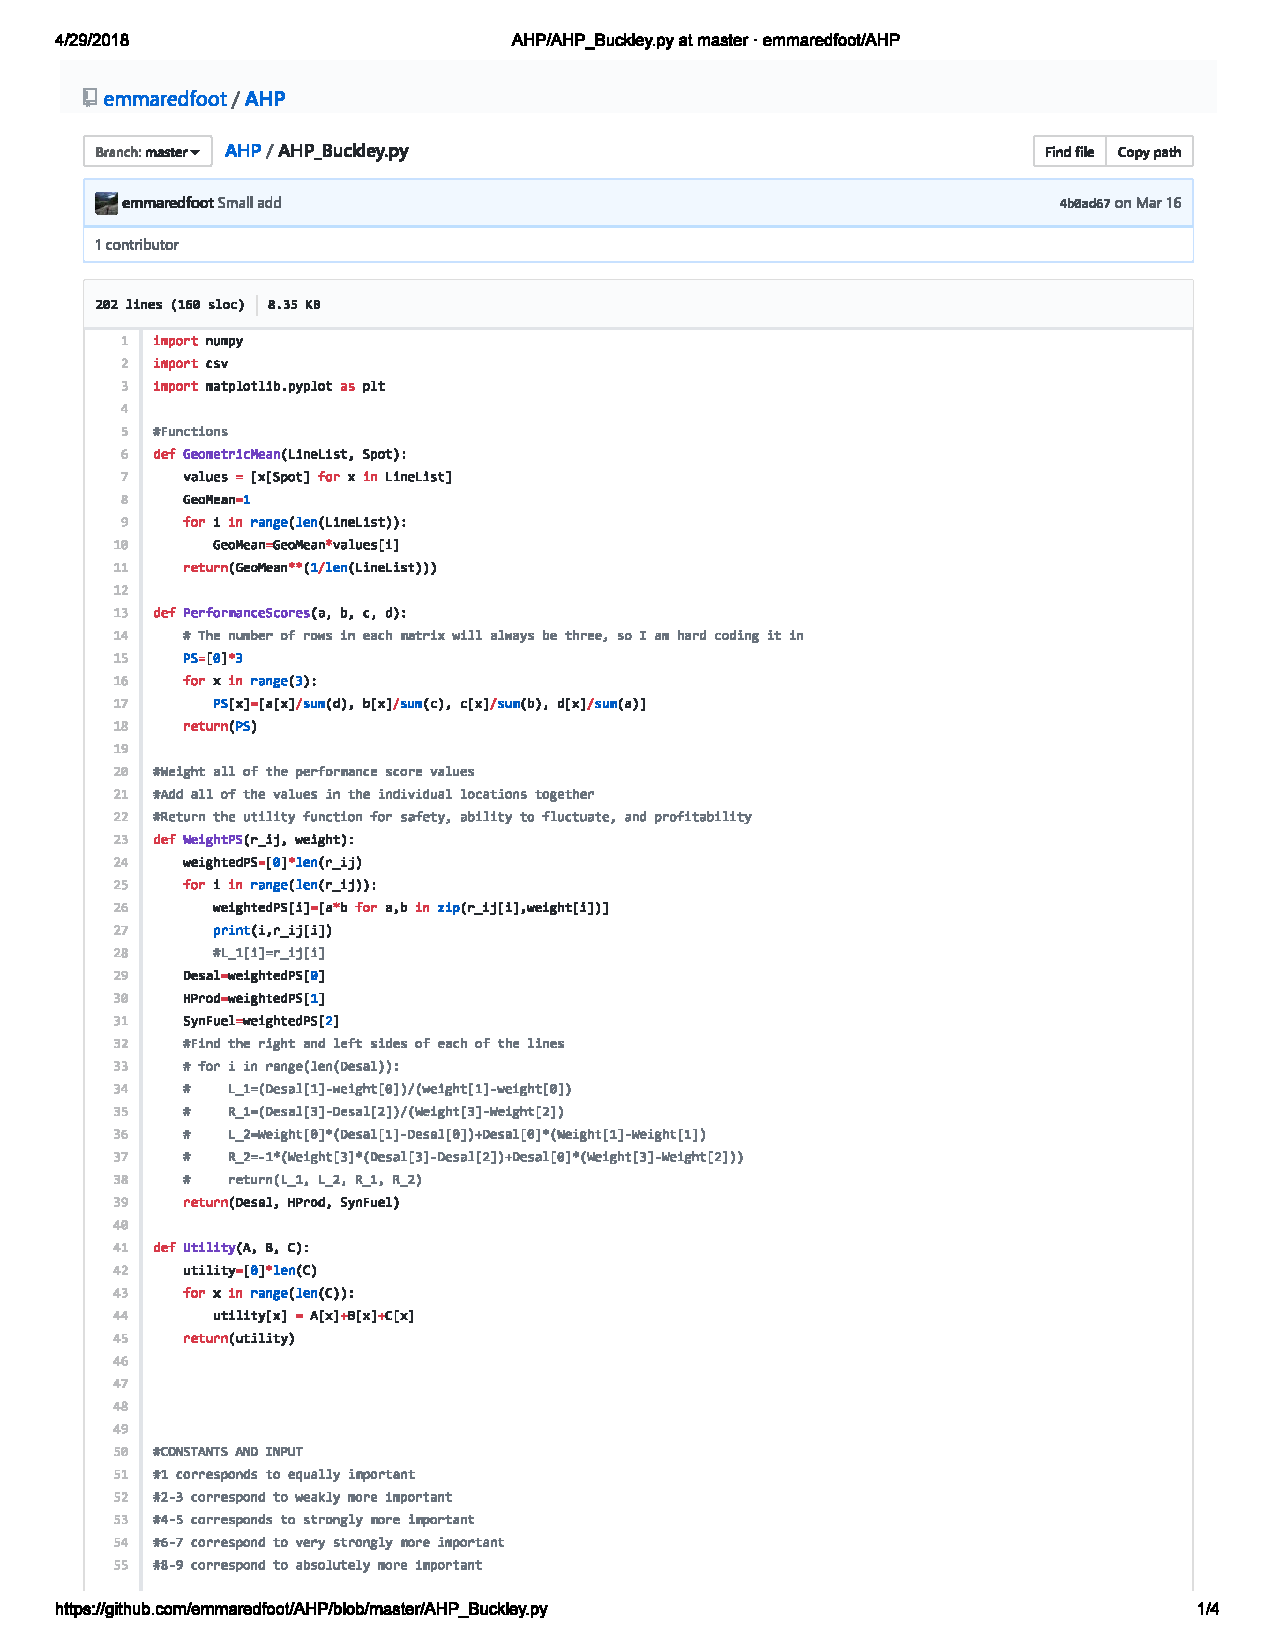
\includepdf{AHP_Buckley_1.pdf}
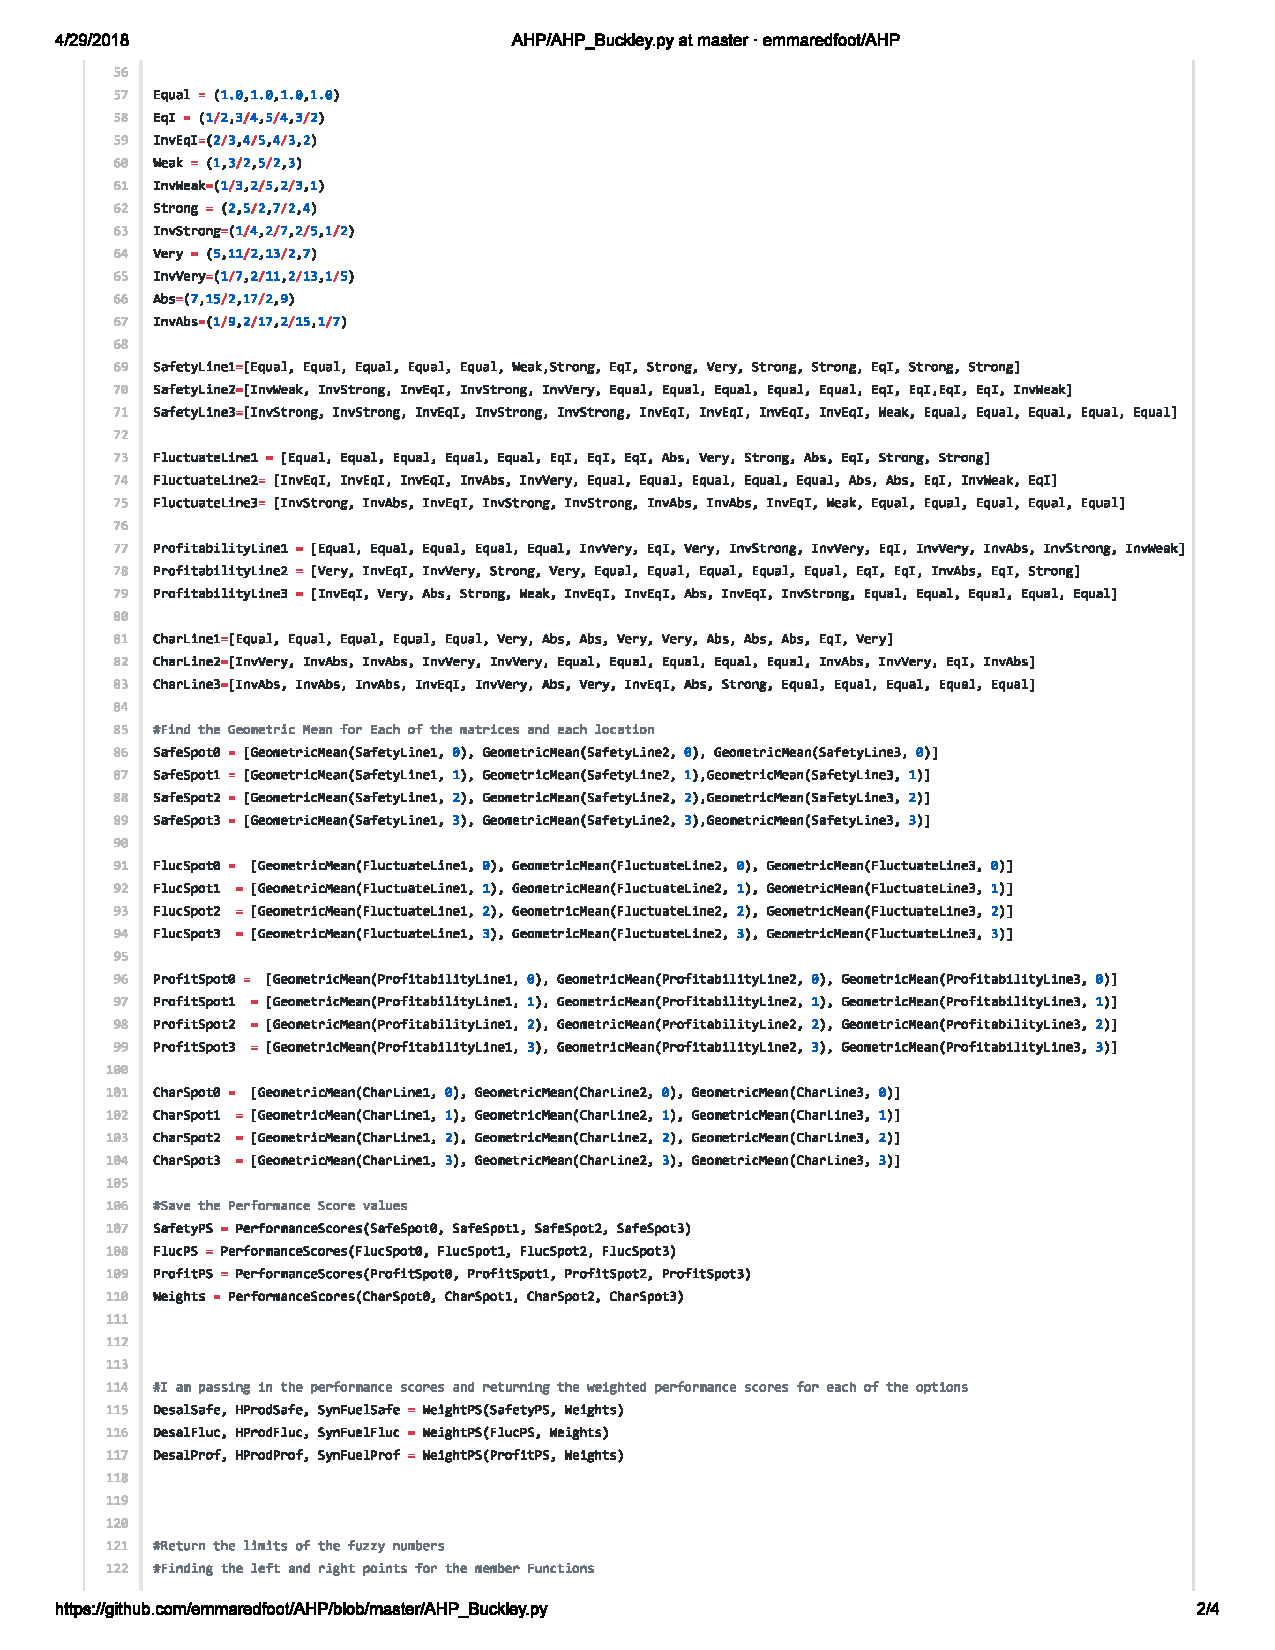
\includepdf{AHP_Buckey_2.pdf}
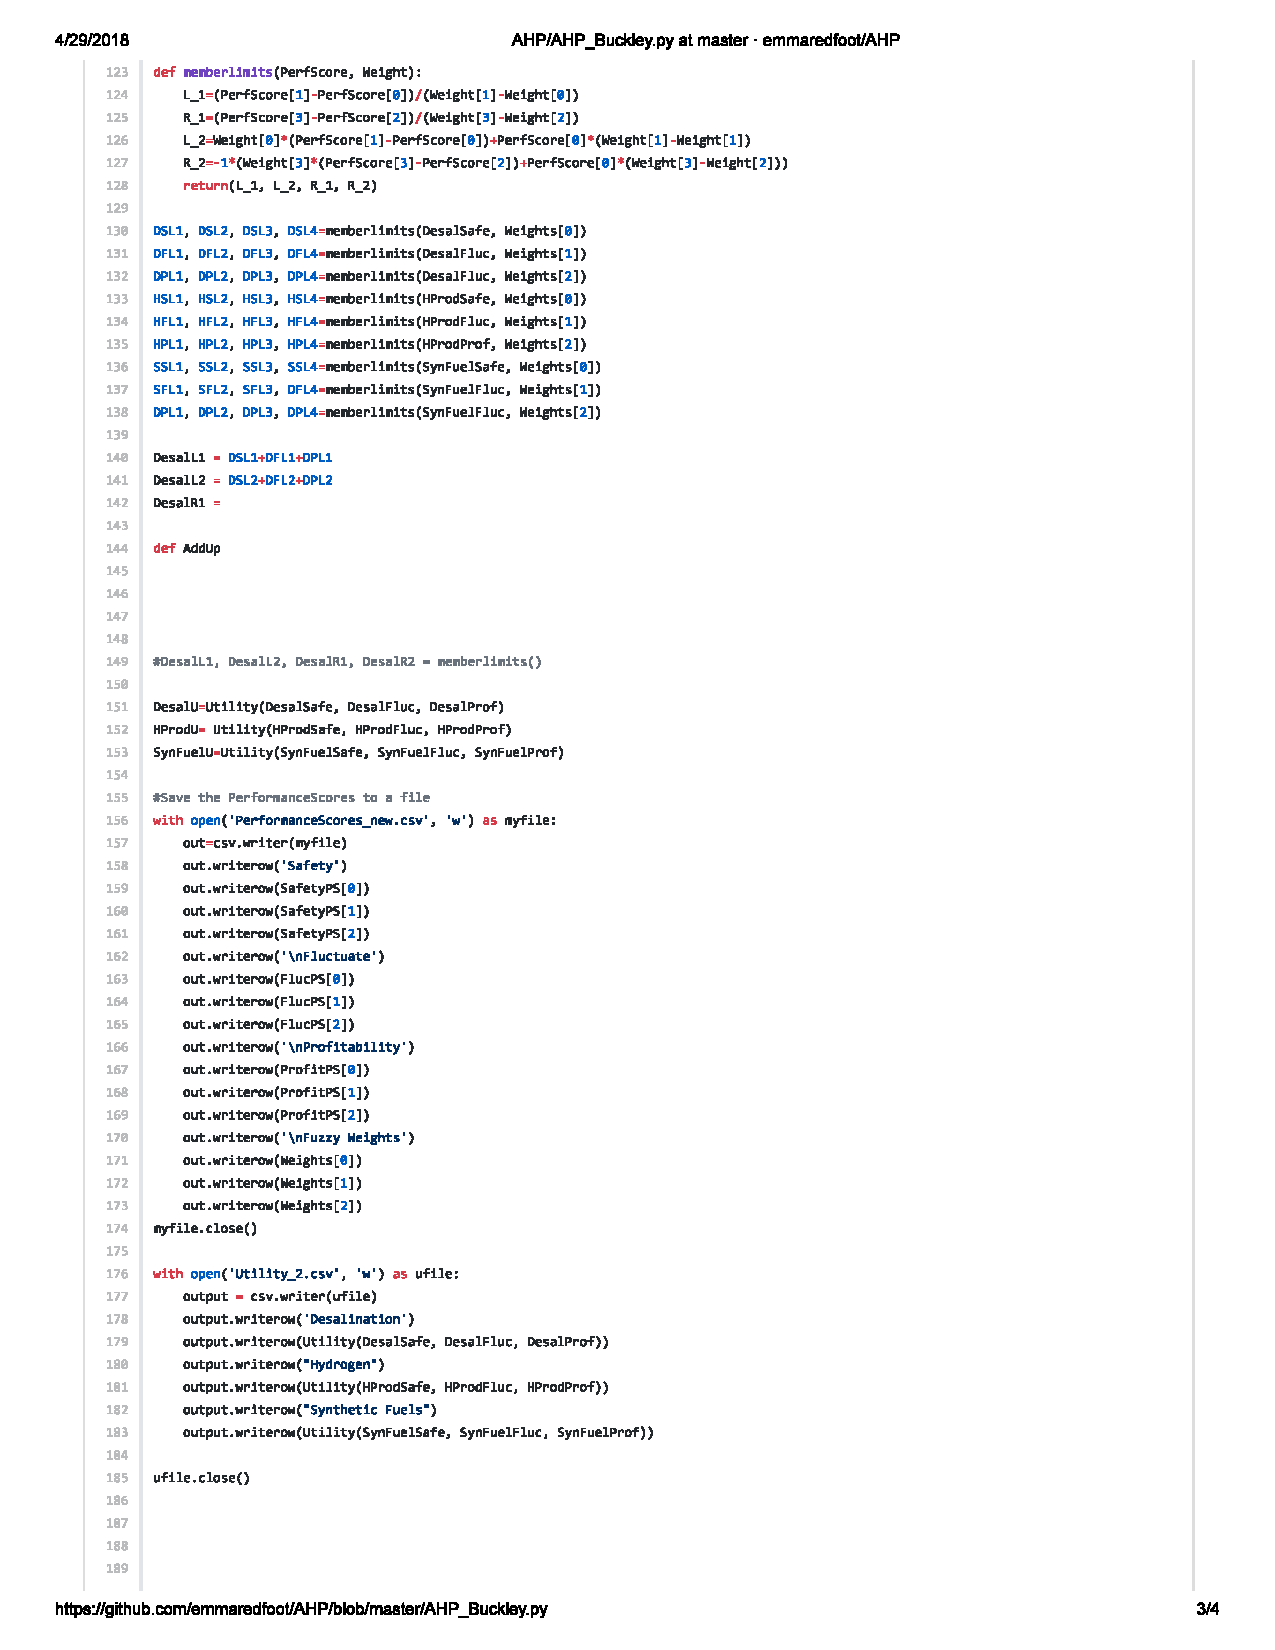
\includepdf{AHP_Buckey_3.pdf}

\chapter{Load Following}

\chapter{Aspen HYSYS}
\begin{figure*}
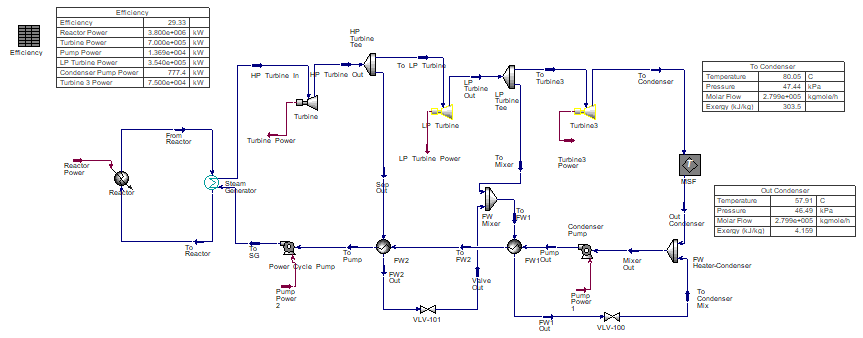
\includegraphics[width=\textwidth]{80PC.PNG}
\caption{\small \sl A much simplified model of the Palo Verde Generating Station's Power Cycle sending 80\degree C heat to the condenser to be used for the multi-stage flash distillation water purification process}
\end{figure*}
\begin{figure*}
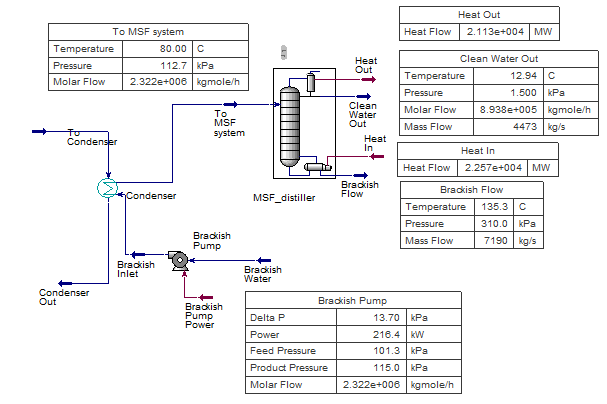
\includegraphics[width=\textwidth]{80MSF.PNG}
\caption{\small \sl A simplified model of a 21 stage multi stage flash distillation system functioning with 80\degree C heat from the reactor to the condenser to be used for the multi-stage flash distillation water purification process}
\end{figure*}
\begin{figure*}
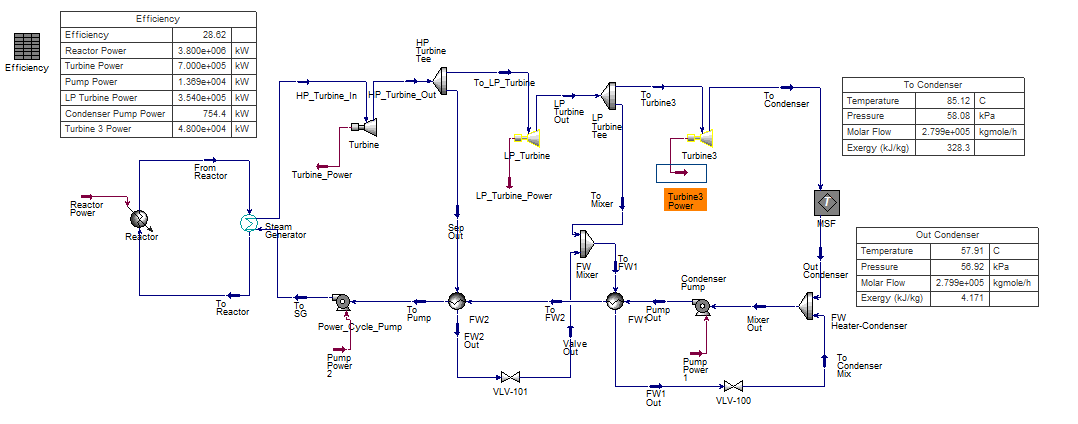
\includegraphics[width=\textwidth]{85PC.PNG}
\caption{\small \sl A much simplified model of the Palo Verde Generating Station's Power Cycle sending 85 \degree C heat to the condenser to be used for the multi-stage flash distillation water purification process}
\end{figure*}
\begin{figure*}
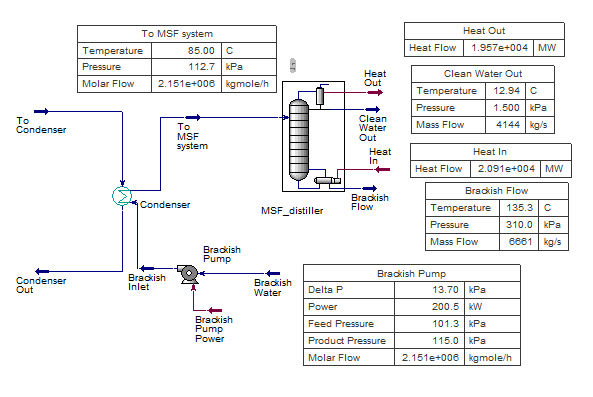
\includegraphics[width=\textwidth]{85MSF.PNG}
\caption{\small \sl A simplified model of a 21 stage multi stage flash distillation system functioning with 85 \degree C heat from the reactor to the condenser to be used for the multi-stage flash distillation water purification process}
\end{figure*}

\begin{figure*}
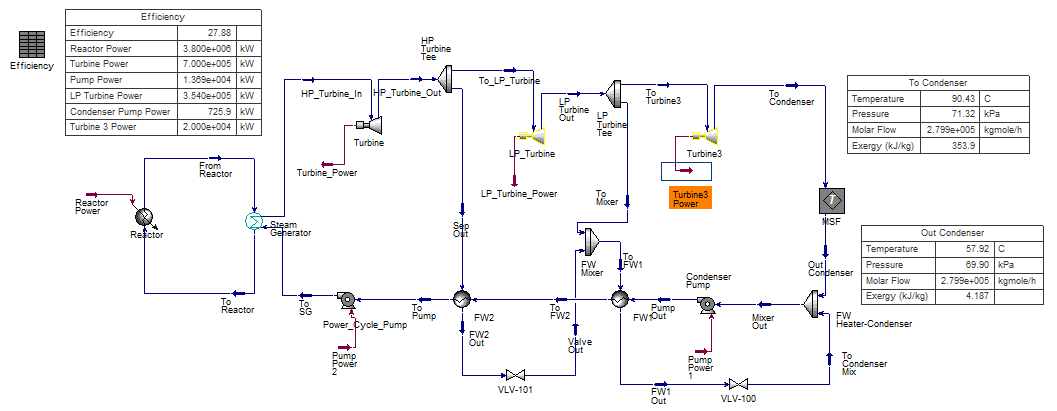
\includegraphics[width=\textwidth]{90PC.PNG}
\caption{\small \sl A much simplified model of the Palo Verde Generating Station's Power Cycle sending 90\degree C heat to the condenser to be used for the multi-stage flash distillation water purification process}
\end{figure*}
\begin{figure*}
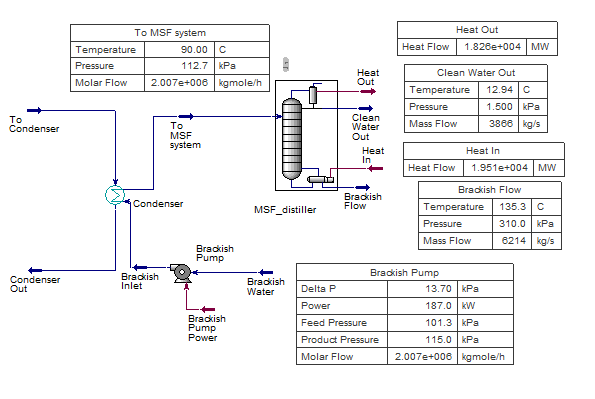
\includegraphics[width=\textwidth]{90MSF.PNG}
\caption{\small \sl A simplified model of a 21 stage multi stage flash distillation system functioning with 90\degree C heat from the reactor to the condenser to be used for the multi-stage flash distillation water purification process}
\end{figure*}
\begin{figure*}
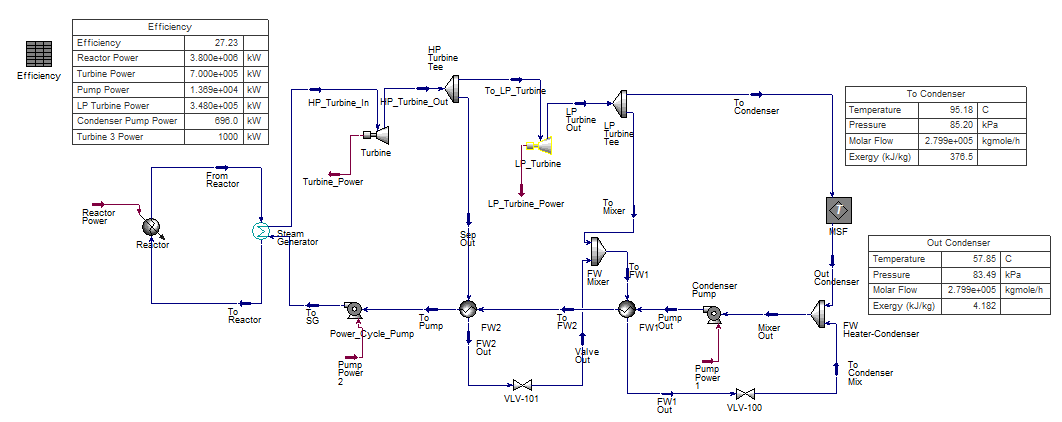
\includegraphics[width=\textwidth]{95PC.PNG}
\caption{\small \sl A much simplified model of the Palo Verde Generating Station's Power Cycle sending 95\degree C heat to the condenser to be used for the multi-stage flash distillation water purification process}
\end{figure*}
\begin{figure*}
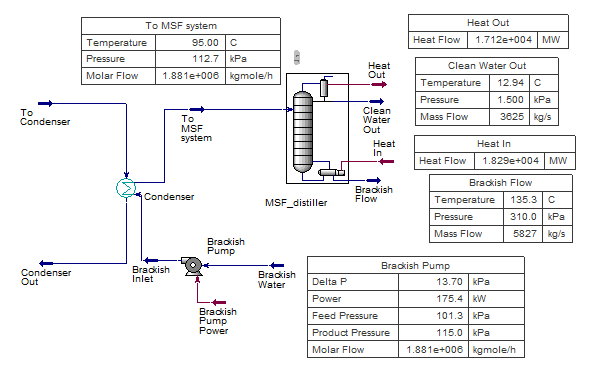
\includegraphics[width=\textwidth]{95MSF.PNG}
\caption{\small \sl A simplified model of a 21 stage multi stage flash distillation system functioning with 95\degree C heat from the reactor to the condenser to be used for the multi-stage flash distillation water purification process}
\end{figure*}
\begin{figure*}
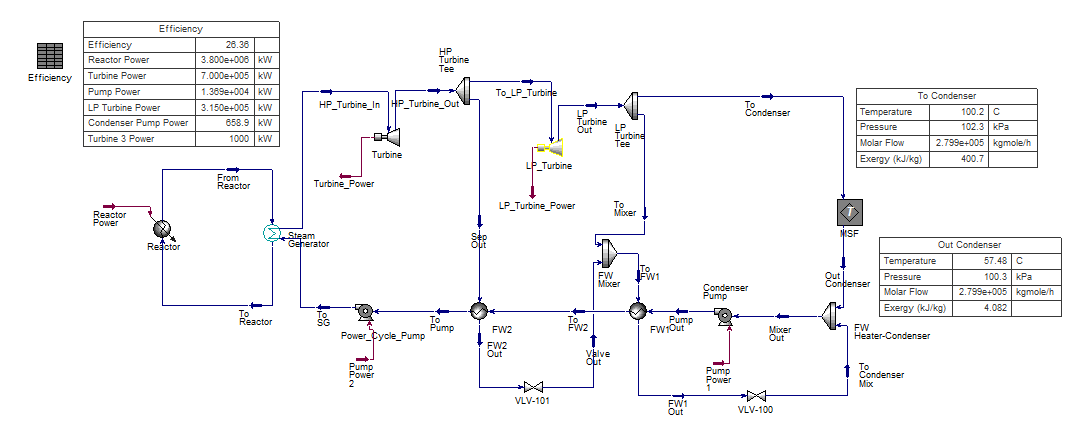
\includegraphics[width=\textwidth]{100PC.PNG}
\caption{\small \sl A much simplified model of the Palo Verde Generating Station's Power Cycle sending 100\degree C heat to the condenser to be used for the multi-stage flash distillation water purification process}
\end{figure*}
\begin{figure*}
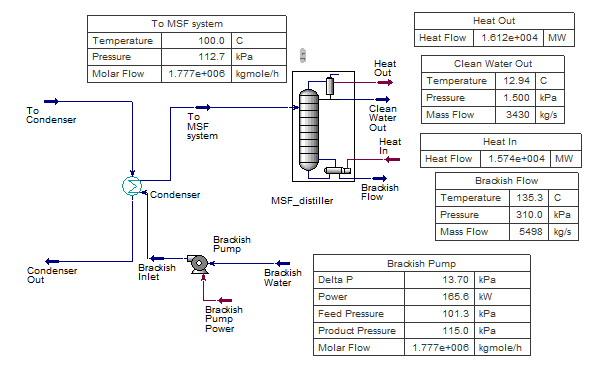
\includegraphics[width=\textwidth]{100MSF.PNG}
\caption{\small \sl A simplified model of a 21 stage multi stage flash distillation system functioning with 100\degree C heat from the reactor to the condenser to be used for the multi-stage flash distillation water purification process}
\end{figure*}
\begin{figure*}
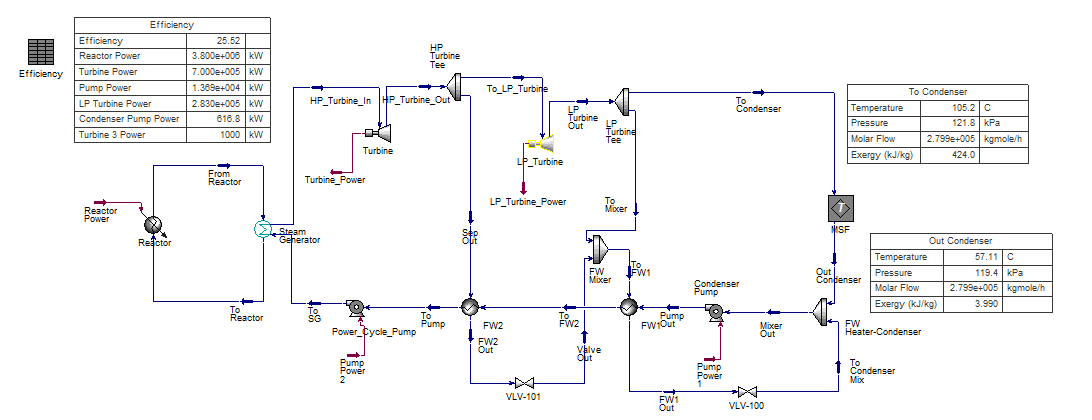
\includegraphics[width=\textwidth]{105PC.PNG}
\caption{\small \sl A much simplified model of the Palo Verde Generating Station's Power Cycle sending 105\degree C heat to the condenser to be used for the multi-stage flash distillation water purification process}
\end{figure*}
\begin{figure*}
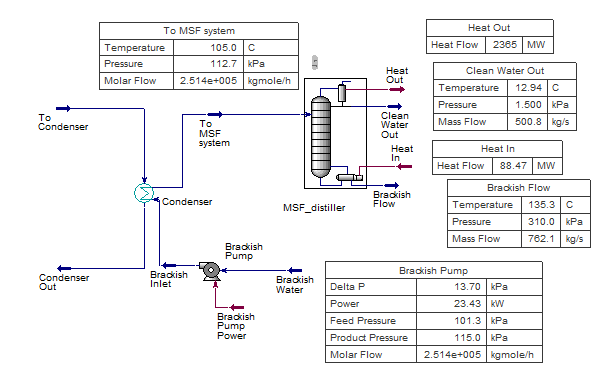
\includegraphics[width=\textwidth]{105MSF.PNG}
\caption{\small \sl A simplified model of a 21 stage multi stage flash distillation system functioning with 105\degree C heat from the reactor to the condenser to be used for the multi-stage flash distillation water purification process}
\end{figure*}
\begin{figure*}
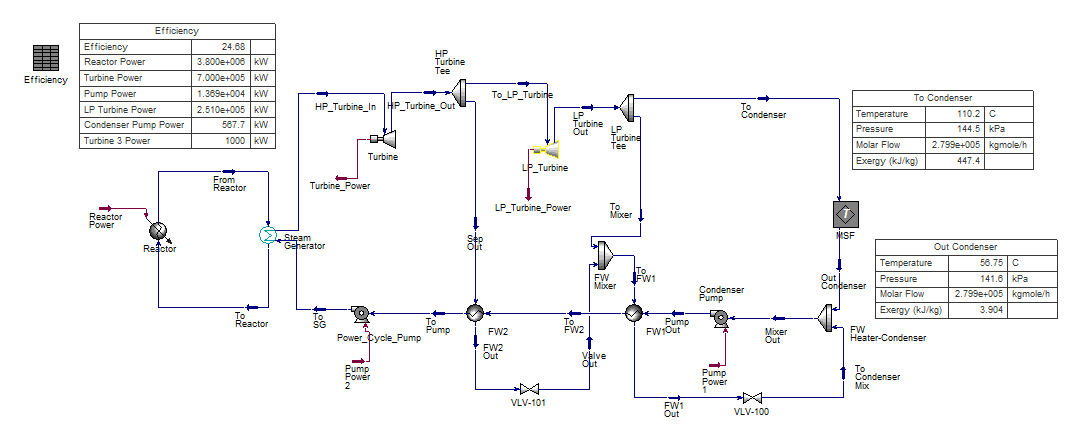
\includegraphics[width=\textwidth]{110PC.PNG}
\caption{\small \sl A much simplified model of the Palo Verde Generating Station's Power Cycle sending 110\degree C heat to the condenser to be used for the multi-stage flash distillation water purification process}
\end{figure*}
\begin{figure*}
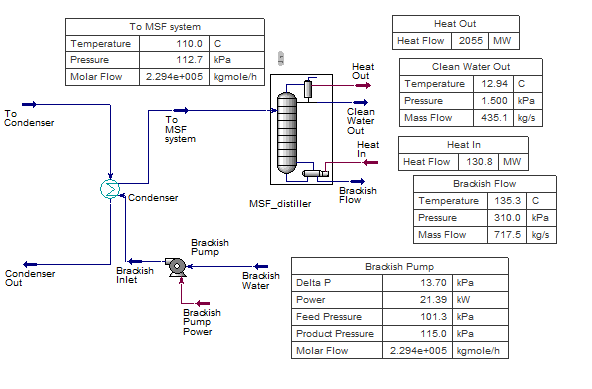
\includegraphics[width=\textwidth]{110MSF.PNG}
\caption{\small \sl A simplified model of a 21 stage multi stage flash distillation system functioning with 110\degree C heat from the reactor to the condenser to be used for the multi-stage flash distillation water purification process}
\end{figure*}

\begin{figure*}
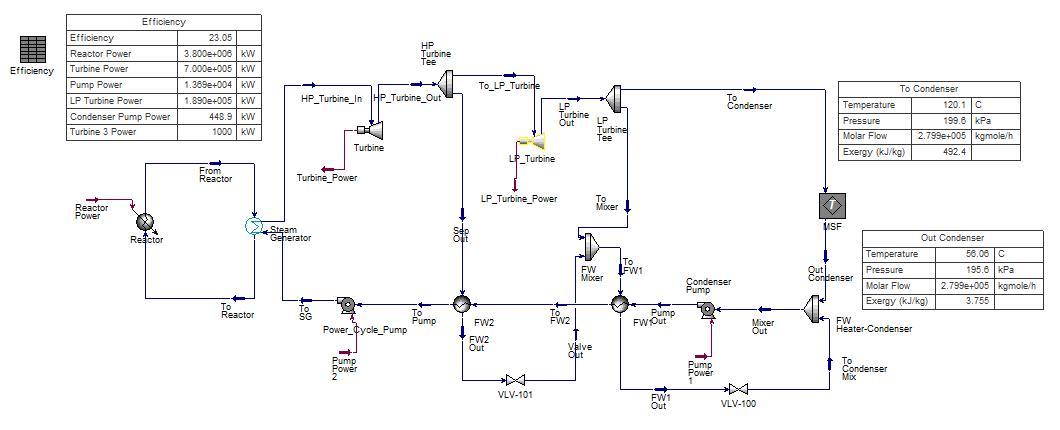
\includegraphics[width=\textwidth]{120PC.PNG}
\caption{\small \sl A much simplified model of the Palo Verde Generating Station's Power Cycle sending 120\degree C heat to the condenser to be used for the multi-stage flash distillation water purification process}
\end{figure*}
\begin{figure*}
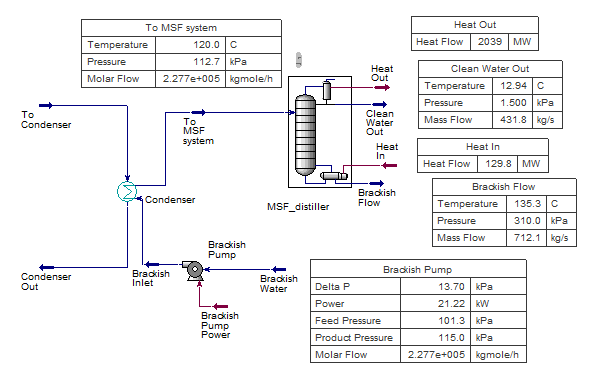
\includegraphics[width=\textwidth]{120MSF.PNG}
\caption{\small \sl A simplified model of a 21 stage multi stage flash distillation system functioning with 120\degree C heat from the reactor to the condenser to be used for the multi-stage flash distillation water purification process}
\end{figure*}
\begin{figure*}
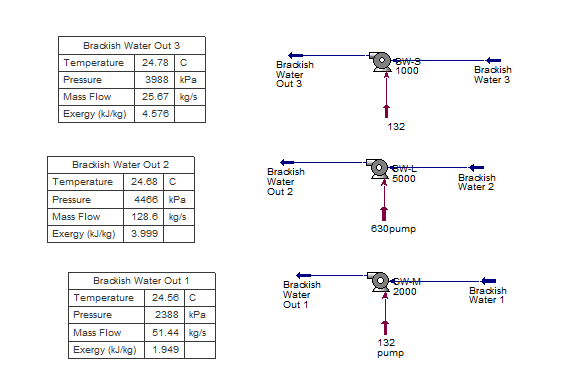
\includegraphics[width=\textwidth]{RO_3Pumps.PNG}
\caption{\small \sl Three pumps which are marketed for reverse osmosis systems by IDE Progreen}
\end{figure*}

\newpage

\section{Aspen HYSYS Water Composition Calculation}

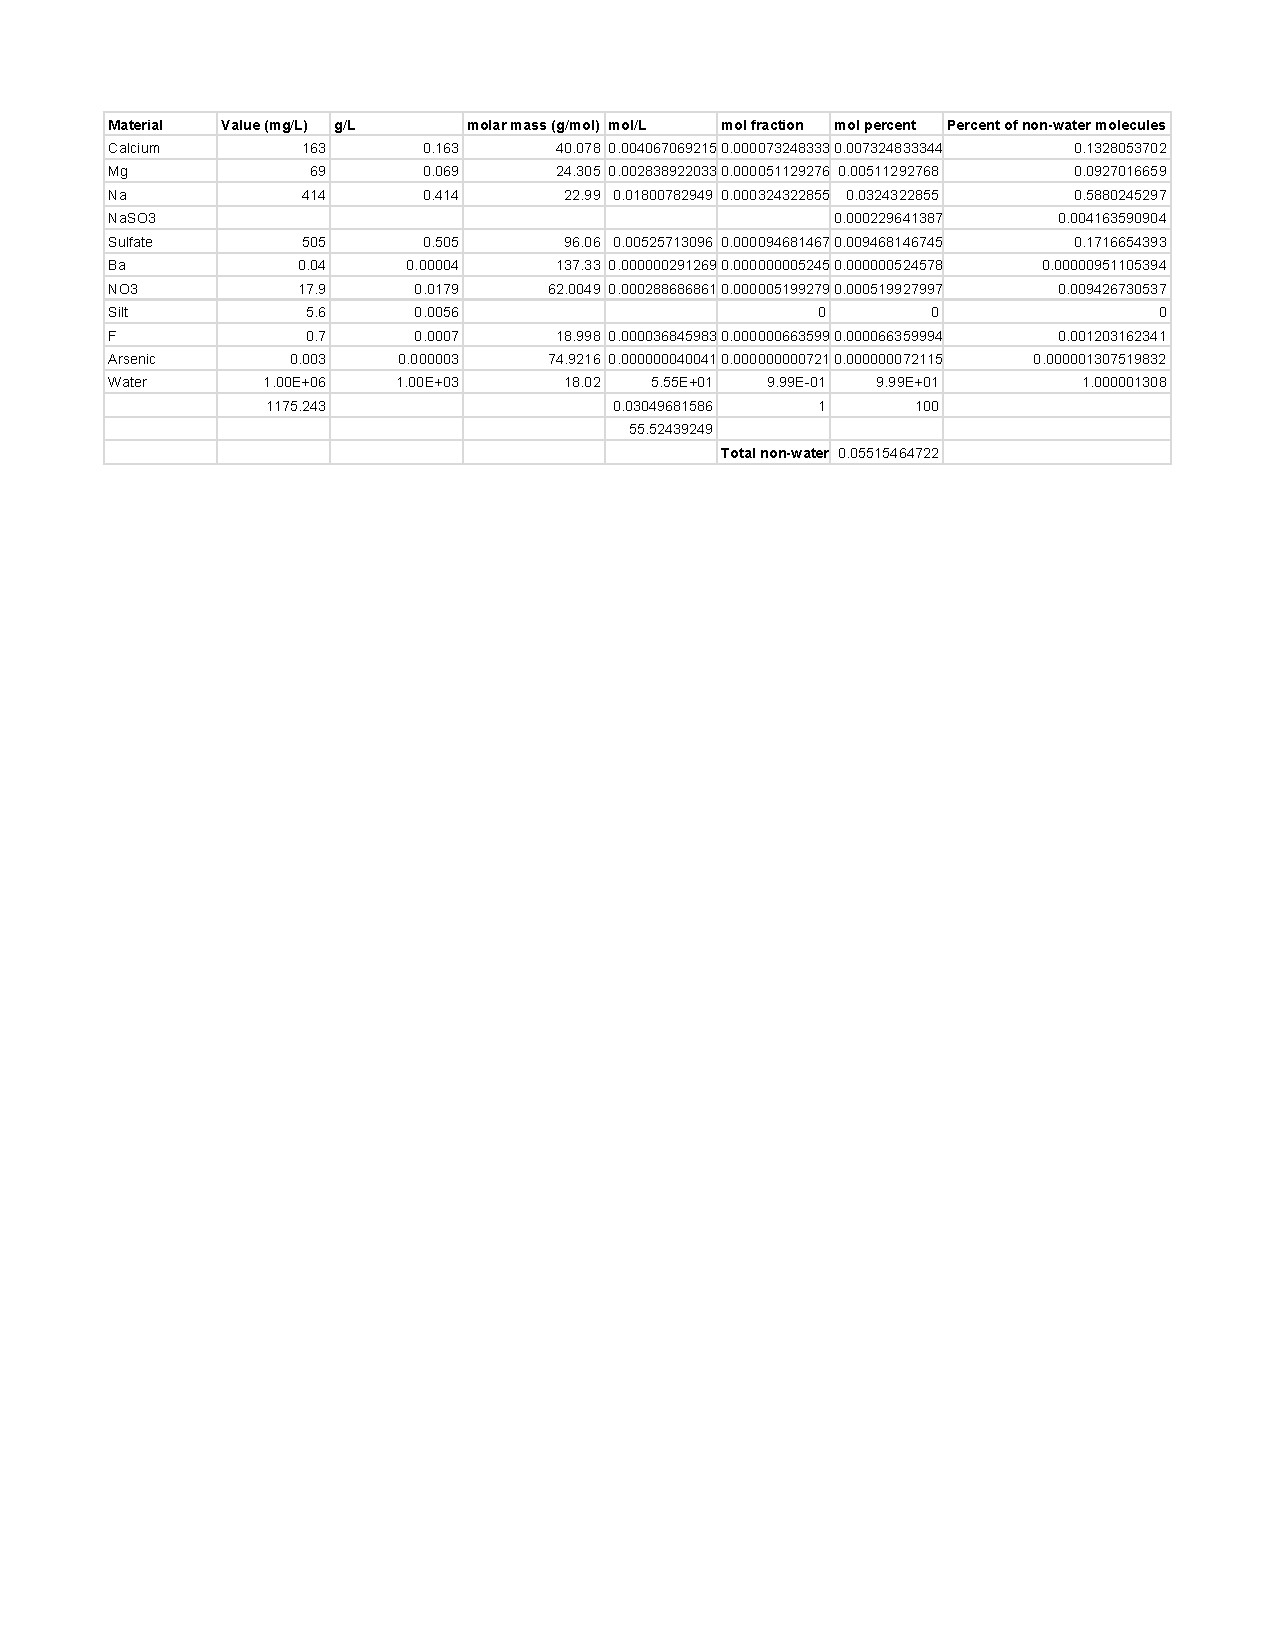
\includepdf{Brackish_-_Sheet1.pdf}

\chapter{RAVEN}
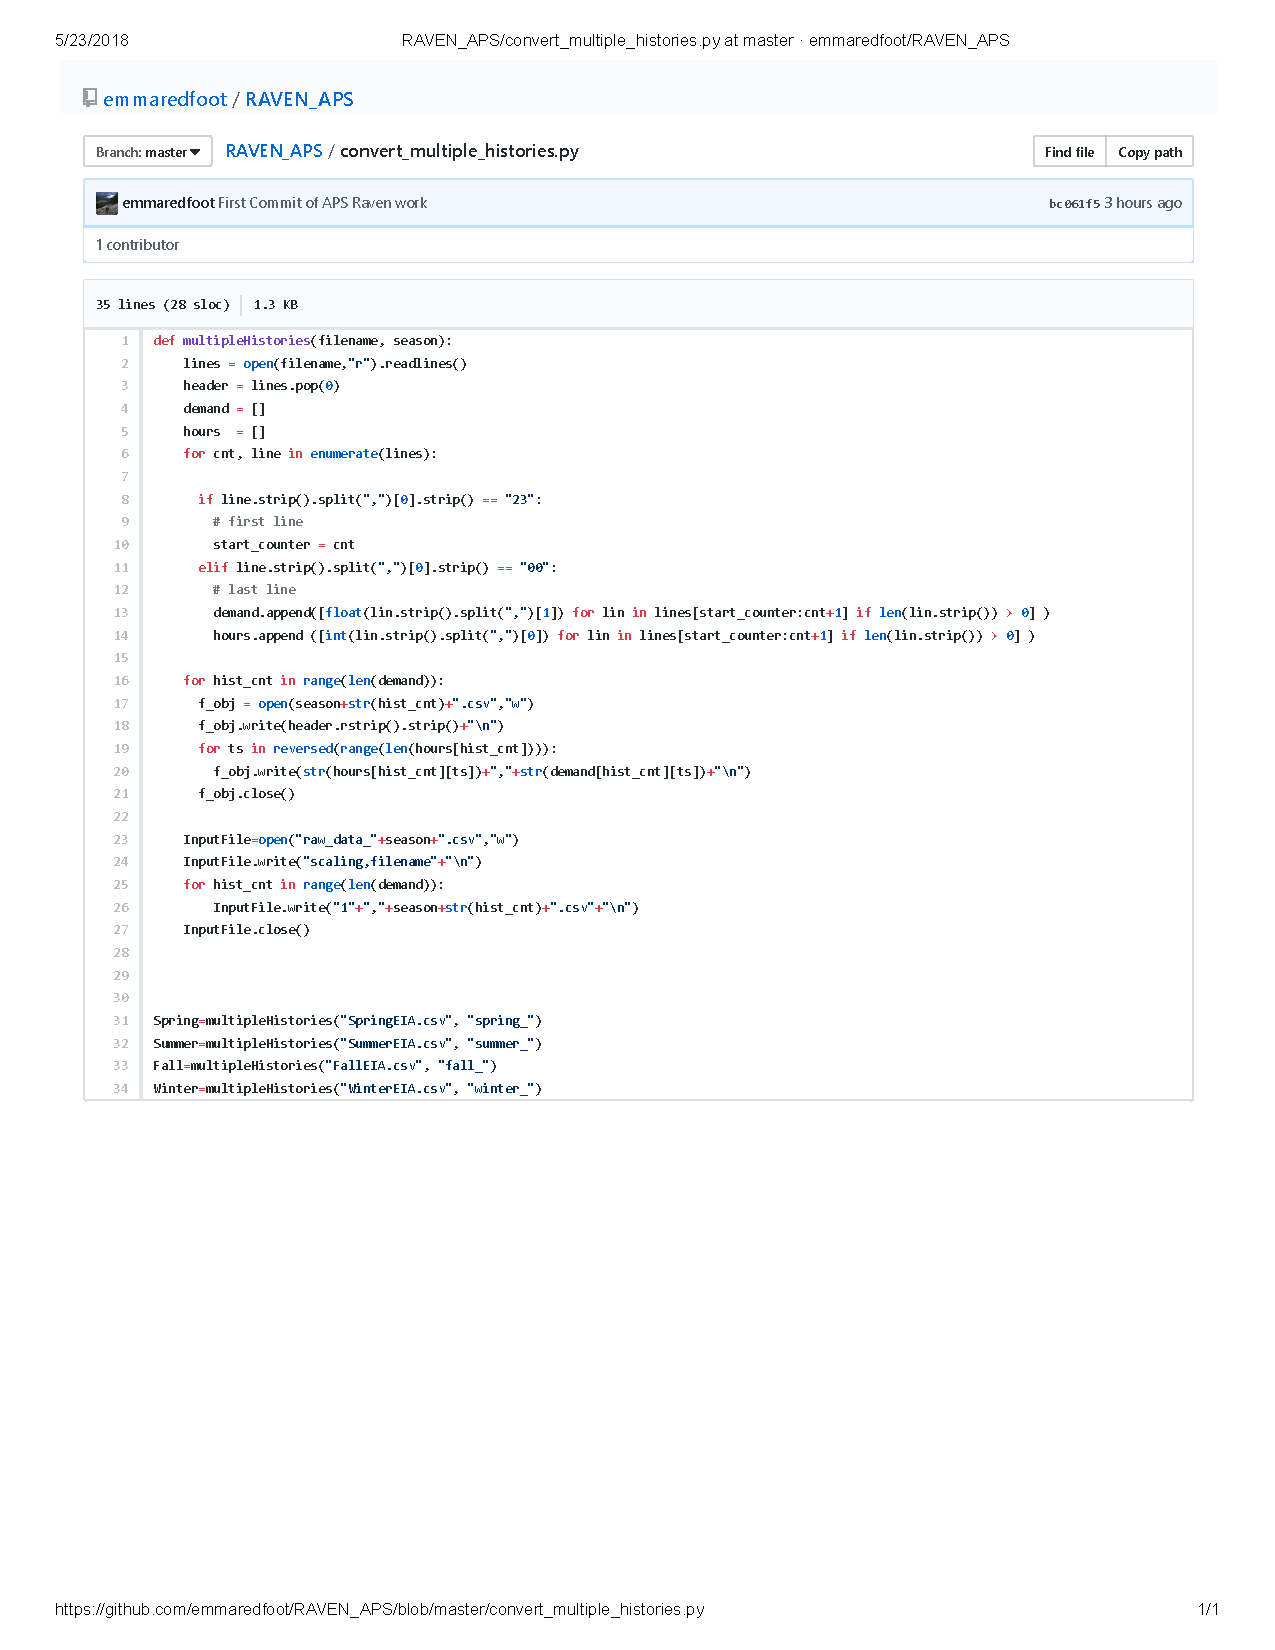
\includepdf{convert_multiple_histories.pdf}
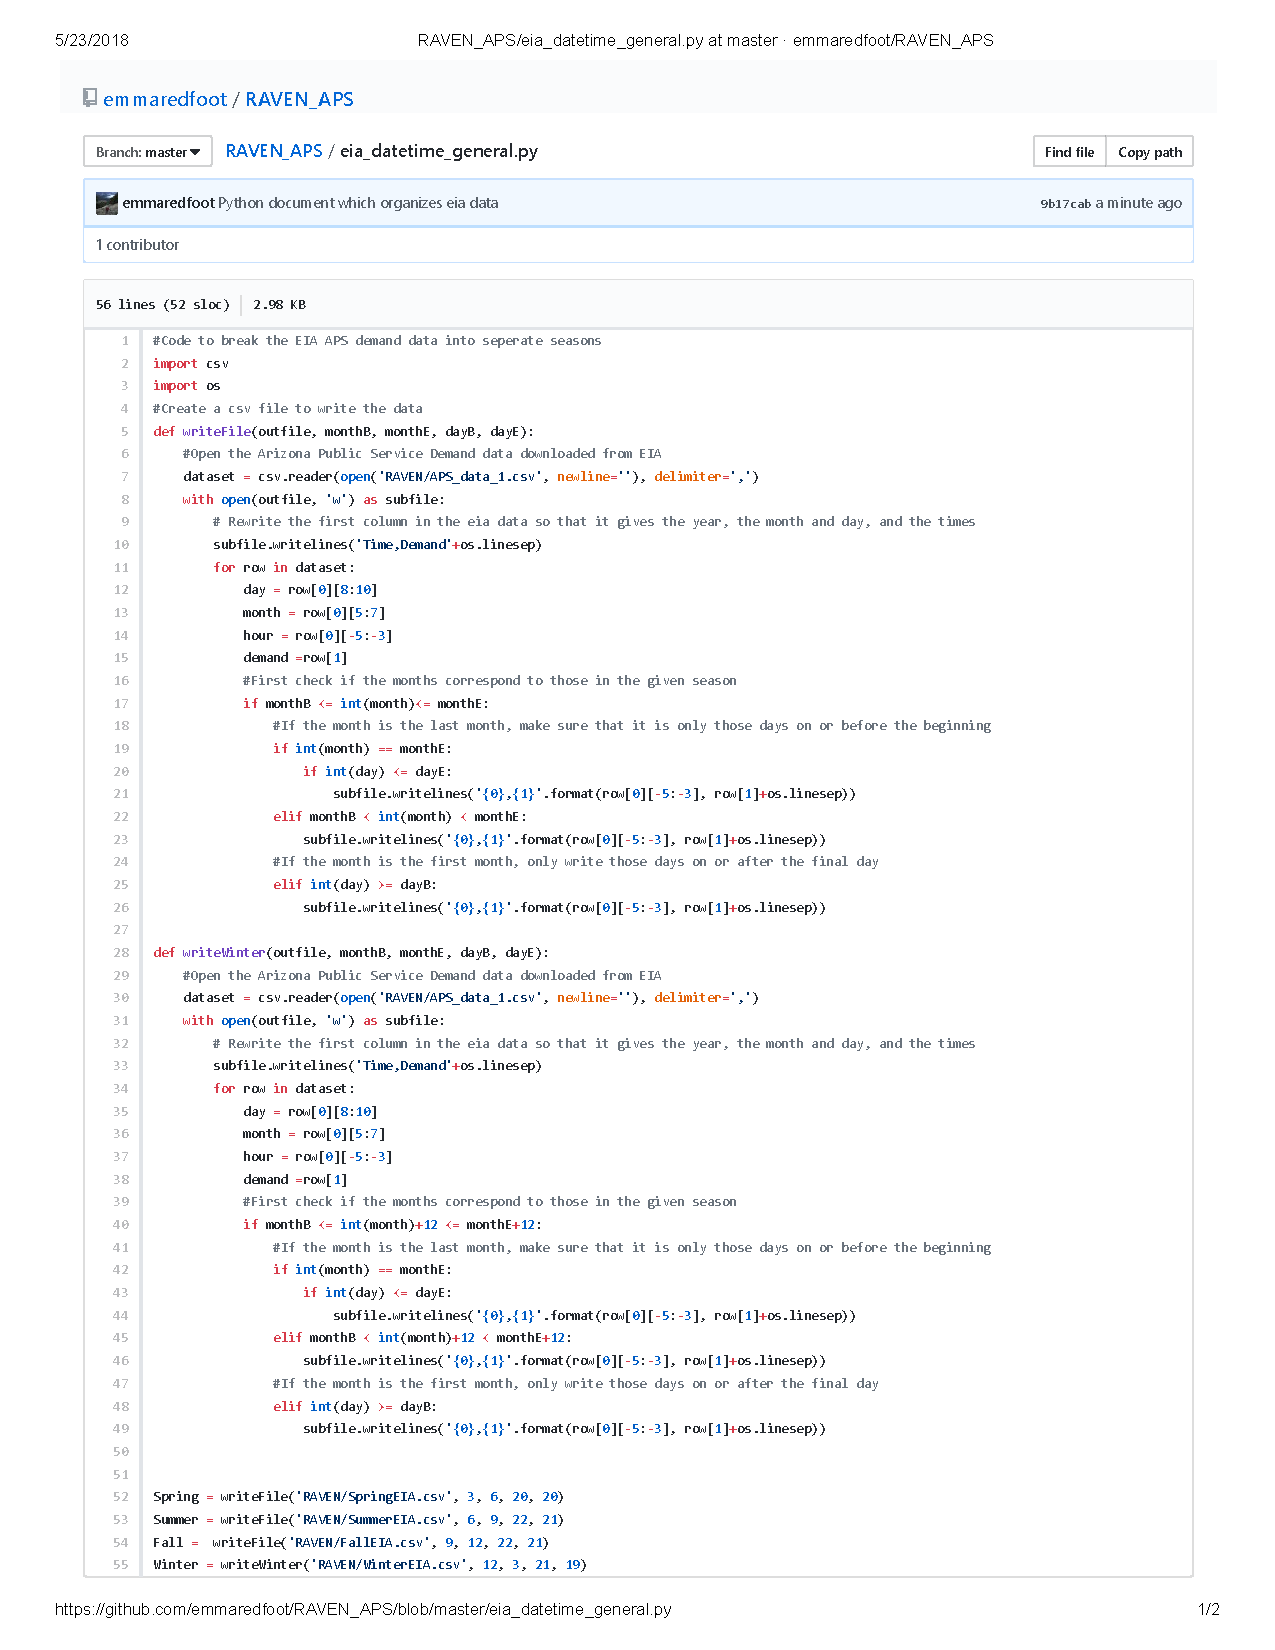
\includepdf{eia_data_python.pdf}

% ** This is an example of a YAML file listing, but it could be anythig, e.g full experiment results, or list of equipment used. **
% \clearpage
% \chapter{Exercise Specification}
% \lstinputlisting[firstline=56, firstnumber=1, language=yaml,caption=Exercise Specification]{Specifications/exercise-specification.yaml}

% ** Example of a Python script code listing **
% \clearpage
% \chapter{vsphere-info Script Source Code}
% \lstinputlisting[firstline=16, firstnumber=1, language=python, caption=vsphere-info script]{Code/scripts/vsphere_info.py}



\end{document}

% ** DO NOT PUT ANYTHING AFTER THE END OF THE DOCUMENT! **